% ****************************************************************************************** % Dissertation template and document class for Princeton University
% Author  : Jeffrey Scott Dwoskin <jdwoskin@princeton.edu>
% Adapted from: http://www.math.princeton.edu/graduate/tex/puthesis.html
% ****************************************************************************************** %

\newcommand{\E}{\mathrm{E}}
\newcommand{\Var}{\mathrm{Var}}
\newcommand{\Cov}{\mathrm{Cov}}



%%% For print copies
%% set 'singlespace' option to set entire thesis to single space, and define "\printmode" to remove all hyperlinks for printed copies of the thesis. Delete all output files before changing this mode -- it will turn hyperref package on and off
%\documentclass[12pt,lot, lof, singlespace]{puthesis}
%\newcommand{\printmode}{}

%%% For the electronic copy, use doublespacing, define "\proquestmode" to use outlined links, instead of colored links. 
\documentclass[12pt,lot, lof]{puthesis}
\newcommand{\proquestmode}{}
% I prefer proquestmode to be off for electronic copies for normal use, since the colored links are less distracting. However when printed in black and white, the colored links are difficult to read. 

%%% For early drafts without some of the frontmatter
% Also see the "ifodd" command below to disable more frontmatter
%\documentclass[12pt]{puthesis}

%%%%%%%%%%%%%%%%%%%%%%%%%%%%%%%%%%%%%%%%%%%%%%%%%%%%%%%%%%%%%\
%%%% Author & title page info

\title{A High-Dimensional Visualization System with Applications in Portfolio 
Management}

\submitted{June 2017}  % degree conferral date (January, April, June, 
%September, or November)
\copyrightyear{2017}  % year in which the copyright is secured by publication of the dissertation.
\author{Amy Tian}
\adviser{Professor Han Liu}  %replace with the full name of your adviser
%\departmentprefix{Program in}  % defaults to "Department of", but programs need to change this.
\department{Operations Research and Financial Engineering}

%%%%%%%%%%%%%%%%%%%%%%%%%%%%%%%%%%%%%%%%%%%%%%%%%%%%%%%%%%%%%\
%%%% Tweak float placements
% From: http://mintaka.sdsu.edu/GF/bibliog/latex/floats.html "Controlling LaTeX Floats"
% and based on: http://www.tex.ac.uk/cgi-bin/texfaq2html?label=floats
% LaTeX defaults listed at: http://people.cs.uu.nl/piet/floats/node1.html

% Alter some LaTeX defaults for better treatment of figures:
    % See p.105 of "TeX Unbound" for suggested values.
    % See pp. 199-200 of Lamport's "LaTeX" book for details.
    %   General parameters, for ALL pages:
    \renewcommand{\topfraction}{0.85}	% max fraction of floats at top
    \renewcommand{\bottomfraction}{0.6}	% max fraction of floats at bottom
    %   Parameters for TEXT pages (not float pages):
    \setcounter{topnumber}{2}
    \setcounter{bottomnumber}{2}
    \setcounter{totalnumber}{4}     % 2 may work better
    \setcounter{dbltopnumber}{2}    % for 2-column pages
    \renewcommand{\dbltopfraction}{0.66}	% fit big float above 2-col. text
    \renewcommand{\textfraction}{0.15}	% allow minimal text w. figs
    %   Parameters for FLOAT pages (not text pages):
    \renewcommand{\floatpagefraction}{0.66}	% require fuller float pages
	% N.B.: floatpagefraction MUST be less than topfraction !!
    \renewcommand{\dblfloatpagefraction}{0.66}	% require fuller float pages

% The documentclass already sets parameters to make a high penalty for widows and orphans. 

%%%%%%%%%%%%%%%%%%%%%%%%%%%%%%%%%%%%%%%%%%%%%%%%%%%%%%%%%%%%%\
%%%% Use packages

%\usepackage{amsfonts}

%%% For figures
\usepackage{graphicx}
%\usepackage{subfig,rotate}

%%% For code
\usepackage{listings}
\usepackage{setspace}
\usepackage{amsmath}
\usepackage{algorithm}
\usepackage[noend]{algpseudocode}
\usepackage{float}
\usepackage{amsfonts}
\usepackage{pdflscape}
%\usepackage{algorithm2e}

%%% for comments
\usepackage{verbatim}

%%% For tables
\usepackage{multirow}
% Longtable lets you have tables that span multiple pages.
\usepackage{longtable}

% Booktabs produces far nicer tables than the standard LaTeX tables.
%   see: http://en.wikibooks.org/wiki/LaTeX/Tables
\usepackage{booktabs}

%set parameters for longtable:
% default caption width is 4in for longtable, but wider for normal tables
\setlength{\LTcapwidth}{\textwidth}



%%%%%%%%%%%%%%%%%%%%%%%%%%%%%%%%%%%%%%%%%%%%%%%%%%%%%%%%%%
%%% Printed vs. online formatting
\ifdefined\printmode


%\section{Switching Formats}
%When switching \texttt{printmode} on and off, you may need to delete the 
%output .aux files to get the document code to compile correctly. This is 
%because the hyperref package is switched off for \texttt{printmode}, but this 
%package inserts extra tags into the contents lines in the auxiliary files for 
%PDF links, and these can cause errors when the package is not used.






% Printed copy
% url package understands urls (with proper line-breaks) without hyperlinking them
\usepackage{url}


\else

\ifdefined\proquestmode
%ProQuest copy -- http://www.princeton.edu/~mudd/thesis/Submissionguide.pdf

% ProQuest requires a double spaced version (set previously). They will take an electronic copy, so we want links in the pdf, but also copies may be printed or made into microfilm in black and white, so we want outlined links instead of colored links.
\usepackage{hyperref}
\hypersetup{bookmarksnumbered}

% copy the already-set title and author to use in the pdf properties
\makeatletter
\hypersetup{pdftitle=\@title,pdfauthor=\@author}
\makeatother

\else
% Online copy

% adds internal linked references, pdf bookmarks, etc

% turn all references and citations into hyperlinks:
%  -- not for printed copies
% -- automatically includes url package
% options:
%   colorlinks makes links by coloring the text instead of putting a rectangle around the text.
\usepackage{hyperref}
\hypersetup{colorlinks,bookmarksnumbered}

% copy the already-set title and author to use in the pdf properties
\makeatletter
\hypersetup{pdftitle=\@title,pdfauthor=\@author}
\makeatother

% make the page number rather than the text be the link for ToC entries
%\hypersetup{linktocpage}
\fi % proquest or online formatting
\fi % printed or online formatting


%%%%%%%%%%%%%%%%%%%%%%%%%%%%%%%%%%%%%%%%%%%%%%%%%%%%%%%%%%%%%\
%%%% Define commands

% Define any custom commands that you want to use.
% For example, highlight notes for future edits to the thesis
%\newcommand{\todo}[1]{\textbf{\emph{TODO:}#1}}


% create an environment that will indent text
% see: http://latex.computersci.org/Reference/ListEnvironments
% 	\raggedright makes them left aligned instead of justified
\newenvironment{indenttext}{
    \begin{list}{}{ \itemsep 0in \itemindent 0in
    \labelsep 0in \labelwidth 0in
    \listparindent 0in
    \topsep 0in \partopsep 0in \parskip 0in \parsep 0in
    \leftmargin 1em \rightmargin 0in
    \raggedright
    }
    \item
  }
  {\end{list}}

% another environment that's an indented list, with no spaces between items -- if we want multiple items/lines. Useful in tables. Use \item inside the environment.
% 	\raggedright makes them left aligned instead of justified
\newenvironment{indentlist}{
    \begin{list}{}{ \itemsep 0in \itemindent 0in
    \labelsep 0in \labelwidth 0in
    \listparindent 0in
    \topsep 0in \partopsep 0in \parskip 0in \parsep 0in
    \leftmargin 1em \rightmargin 0in
    \raggedright
    }

  }
  {\end{list}}



%%%%%%%%%%%%%%%%%%%%%%%%%%%%%%%%%%%%%%%%%%%%%%%%%%%%%%%%%%%%%\
%%%% Front-matter

% For early drafts, you may want to disable some of the frontmatter. Simply change this to "\ifodd 1" to do so.
\ifodd 0
% front-matter disabled while writing chapters
\renewcommand{\maketitlepage}{}
\renewcommand*{\makecopyrightpage}{}
\renewcommand*{\makeabstract}{}

% you can just skip the \acknowledgements and \dedication commands to leave out these sections.

\else


\abstract{
% Abstract can be any length, but should be max 350 words for a Dissertation for ProQuest's print indicies (150 words for a Master's Thesis) or it will be truncated for those uses.
Often in modern multivariate analyses, data analysts rely solely on statistical
estimators to explore the data. We are interested in visualizing 
high-dimensional correlation graphs as a way to verify numerical tests of 
dependence, which have far-reaching financial implications. High-dimensional 
visualization is problematic because (1) the number of plots to sort through 
increases quadratically as the number of variables increase, (2) it is tedious 
to verify numerical results with visual results and vice versa. We 
present a visualization tool that actively learns user preferences, applies 
the fitted classifier to unlabeled data, and outputs the difference among the 
numerical graph $G^{\text{num}}=(V,E^{\text{num}})$ and the visual graph 
$G=(V,E)$. 
As a specific response to the aforementioned problems, we focus on 
the active learning and graph comparison components of the visualization 
system. A simulation study with parameters that mimic the intended qualities of 
the system selected uncertainty sampling as the best procedure for use in the 
selection of healthcare stocks for a portfolio. Various graph summarization 
metrics are compiled to compute the difference between two graphs, and a 
procedure for selecting the most similar graph pairs given the differences is 
proposed and verified. 
Furthermore, we propose a simple but effective stock selection procedure to 
select a ``buy and hold'' portfolio of the $k$ stocks which are most 
uncorrelated with each other given a correlation graph, a proxy for 
independence. The healthcare stock price data is run through the visualization 
system, stocks are selected, and the portfolios' yearly returns are compiled. 
The results indicate that the portfolio 
corresponding to the numerical correlation graph which most resembles the 
visual correlation graph is the top performer. 
The visualization tool provides a simple and 
intuitive way to improve predictive and portfolio management methods in the 
financial industry. Moreover, it increases standardization in the data analysis 
process, thereby increasing accountability in an industry where ambiguity can 
mean a global financial crisis.

}

\acknowledgements{
%I would like to thank...
First, I would like to thank my advisor, Professor Han Liu, for his 
guidance and expertise.

I would like to thank Kevin for his patience, feedback, and for being a 
friendly Munchlax. 

I would like to thank Tony for emergency kittens and delicious weekend noms.

I would like to thank my sister, Elizabeth, for being a magical friend 
and thesis fairy. I wish you the best of luck with your own thesis endeavors 
two years down the road. 
I would like to thank my younger brothers who are always fun to be around.

Finally, last but not least, I would like to thank my parents for their 
encouragement, support, and unconditional love. 
}

\dedication{To my family.}

\fi  % disable frontmatter


%%%%%%%%%%%%%%%%%%%%%%%%%%%%%%%%%%%%%%%%%%%%%%%%%%%%%%%%%%%%%\
%%%% Hide some chapters

%%% If you want to produce a pdf that includes only certain chapters, specify them with includeonly, in addition to including all chapters below.
%\includeonly{ch-intro/chapter-intro}
%%% You can also specify multiple chapters.
%\includeonly{ch-intro/chapter-intro,ch-usage/chapter-usage}
%\includeonly{chap1,chap2,chap3}


%%%%%%%%%%%%%%%%%%%%%%%%%%%%%%%%%%%%%%%%%%%%%%%%%%%%%%%%%%%%%
%%%% Notes:

% Footnotes should be placed after punctuation.\footnote{place here.}
% Generally, place citations before the period~\cite{anotherauthor}.
% The proper usage for i.e., and e.g., include commas ``(e.g., option A, option B)''

%%%%%%%%%%%%%%%%%%%%%%%%%%%%%%%%%%%%%%%%%%%%%%%%%%%%%%%%%%%%%
%%%% Import chapters

\begin{document}

\makefrontmatter


% If you've disabled frontmatter, you can insert the toc manually
%\tableofcontents\clearpage

% \include lets us split up the document (and each include starts a new page):

\chapter{Introduction\label{ch:intro}}

\section{Problem statement}
\label{sec:intro:problem}

More than 2.5 quintillion bytes of data are produced daily as the field of data analysis continues to grow. ``Statistical thinking and methodology'' has become the framework for disciplines such as education, agriculture, economics, biology, medicine, astronomy, geology, and physics~\cite{efron1986}, but there is still a lack of accountability and consistency in the field. What is striking in the current practice of data analysis is the lack of progress on this particular subject beyond the development of numerical methods. The rapid increase in computing resources has led to the proliferation of high-dimensional datasets, which are more tedious to efficiently understand patterns in the data and verify numerical estimators. In fact, the ``physical limitations of display devices and our [human's] visual system prevent the direct display and instantaneous recognition of structures with higher dimensions than \textbf{two or three}''~\cite{lius2016} (emphasis mine). One solution is to manually plot each explanatory variable against the response variable, but this becomes computationally tedious and unfeasible to sort through when there are even a few hundred variables. This problem gets even more complicated when considering interaction terms (various transformations or combinations of explanatory variables). Although methods for dimension reduction have been developed~\cite{lius2016}, it is still unclear how the analyst can easily check the resulting model to ensure that the variables which were culled in the dimension reduction process are actually undesirable. Thus, the problem with current high-dimensional visual analysis is two-fold: (1) there are too many potential plots to sort through manually, and (2) it is tedious to verify numerical results with visual results and vice versa. 

In computer science, a framework for ``clean code'' has been extensively documented and is the accepted industry standard for writing, interacting with, and thinking about code. But in empirical data analysis with large datasets, analysts blindly depend on estimators and hypothesis tests to explore the data and have no justification of their analyses aside from asymptotic, mathematical guarantees. Furthermore, since each estimator inherently performs well or poorly under different settings, data analysts are unable to differentiate between the properties intrinsic to the dataset and the spurious properties the estimators added. Little, a Professor of Biostatics at the University of Michigan, notes that ``developing good statistical solutions to real applied problems, based on good science rather than `cookbookery,' is far from easy''~\cite{little2013}. This lack of agreement and ``cookbook'' mentality of data analyses has far-reaching consequences. It is simple to run the data through a list of many estimators and cherry-pick the most ``interesting'' result. Similarly, an analyst can remove undesirable data points without justification or unknowingly fit egregiously incorrect models. Regardless of whether all these situations are performed maliciously or with good intentions, the art of data analysis is unclear without standards. The lack of clear-cut guidelines makes it difficult for analysts to discern the ``truth'' from the data and avoid the aforementioned pitfalls while simultaneously making it difficult for consumers of the resulting analyses to evaluate how trustworthy it is. This mentality arises due to the difficulty in visualizing high-dimensional data; plotting is one of the most consistent and universally interpretable ``sanity checks'' for numerical results.

Consider the following scenario with two different univariate datasets (Appendix~\ref{sec:appendicies:me1plot} and~\ref{sec:appendicies:me2plot}). The problem is if $x$ contains explanatory power of $y$. Common numerical analysis techniques yield the results summarized in Table~\ref{tab:intro:me}.

\tablespacing
% tablespacing is defined by the class to set single spacing for the long table when in doublespacing mode. If the singlespace option is set, this command has no effect.

\begin{longtable}{p{0.3\linewidth} p{0.3\linewidth} p{0.3\linewidth}}
	
	% First page heading
	\caption[Numerical analysis in the univariate case.]{Numerical analysis in the univariate case. The results suggest that the data are uncorrelated. For Dataset 1, refer to Appendix ~\ref{sec:appendicies:me1plot}. For Dataset 2, refer to Appendix ~\ref{sec:appendicies:me2plot}} \label{tab:intro:me}\\
	\toprule
	\textbf{Dependency test} & \textbf{Dataset 1} & \textbf{Dataset 2} \\
	\midrule
	\endfirsthead
	
	% Future page heading
	\caption[]{(continued)}\\
	\toprule
	\textbf{Dependency tests} & \textbf{Dataset 1} & \textbf{Dataset 2} \\
	\midrule
	\endhead
	
	% Page footer
	\midrule
	\multicolumn{3}{r}{(Continued on next page)}\\
	\endfoot
	
	% Last page footer
	\bottomrule
	\endlastfoot
	
	Linear regression & $y=0.461+0.008x$ & $y=-0.131 - 0.2699x$
	\\
	$p$-values & \hspace{0.7cm}(2e-16) (0.911) & \hspace{0.85cm} (0.488) (0.190)
	\\
	Conclusion & Insignificant & Insignificant
	\\
	\cmidrule[0.1pt](l{0.5em}r{0.5em}){1-3}	
	
	ANOVA $p$-value & 0.9109 & 0.1896
	\\
	Conclusion & Insignificant & Insignificant
	\\
	\cmidrule[0.1pt](l{0.5em}r{0.5em}){1-3}
	
	Shapiro $p$-value & 0.5795 & 0.1632
	\\
	Conclusion & Normally-distributed residuals & Normally-distributed residuals
	\\
	\cmidrule[0.1pt](l{0.5em}r{0.5em}){1-3}
	
	Pearson's correlation & -0.1886 & 0.0113
	\\
	$p$-values & 0.1896 & 0.9109
	\\
	Conclusion & Uncorrelated & Uncorrelated
	\\
	
	% the cmidrule here spans both columns but is indented slightly on the left and right. 
	%\cmidrule[0.1pt](l{0.5em}r{0.5em}){1-3}
	
\end{longtable}
\bodyspacing
% bodyspacing restores double spacing or single spacing after the table

Supposing that an analyst must rely on numerical tests alone, the reasonable conclusion to reach would be that $x$ and $y$ are uncorrelated. Given the power to plot quickly and efficiently, however, an analyst would quickly discover that the data exhibits a strong dependency (Figure~\ref{fig:intro:meplot}). There are certainly many more ways to numerically analyze the data, and in retrospect, it can be argued that an analyst might have tried an estimator that captured the dependency properly. Even then, without the ability to plot, the previous numerical results (which were strongly uncorrelated) cast doubt on the sole correlated estimator.

\begin{figure}[htb]
	\begin{center}
		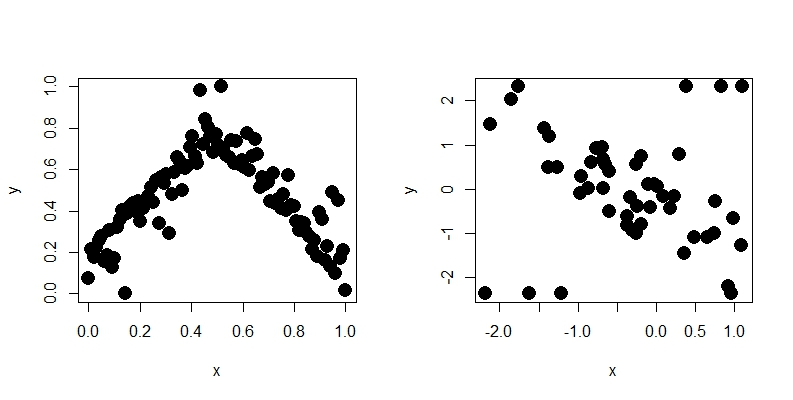
\includegraphics[width=1\linewidth]{ch-intro/figures/me}
		\caption[Visual analysis in the univariate case.]{Visual analysis in the univariate case. The data exhibits a strong visual dependency but fails common numerical tests of dependence (Table~\ref{tab:intro:me}). \textit{Left}: Dataset 1 (Appendix~\ref{sec:appendicies:me1plot}), \textit{Right}: Dataset 2 (Appendix~\ref{sec:appendicies:me2plot})}
		\label{fig:intro:meplot}
	\end{center}
\end{figure}

It is interesting to note that Dataset 2 (Figure~\ref{fig:intro:meplot}, right) is clearly linear yet common tests of linear correlation (linear regression, Pearson's correlation. See Section~\ref{sec:intro:correlation}) are not significantly different from 0 (Table~\ref{tab:intro:me}). Indeed, the data used in these examples was purposefully constructed to be dependent but bypass common tests for dependency. However, if it is possible to construct datasets in one-dimension that evade commonly-used numerical methods, it is believable that it is even easier to construct analogous datasets in higher dimensions. Hence, no such standards of ``clean analysis'' currently exist in data science despite its importance in financial decisions, judicial evidence, government policy, and scientific discovery. Verification of numerical methods is especially important in finance as equity markets are large and involve billions of dollars; portfolio selection often involves determining the relationship among as many stocks as possible in order to be thorough and achieve the best possible portfolio. 
\section{Motivating example 1}
\label{sec:intro:me1}

With the univariate case (one observation variable $x$ and one response variable $y$), we generate and alter a sample of 100 data points from a normal distribution. We have developed this data to illustrate an interesting phenomenon. Even in this simplistic setting, numerical tools commonly used in regression analysis can fail dramatically when not accompanied by corresponding visualization tools.

For the purpose of this example, imagine that a data analyst cannot produce any plots in the analysis, and the desired question to answer is if $x$ contains explanatory power of $y$. The natural thing to try first is to fit simple linear regression and determine the significance of its coefficient. Doing this, the ANOVA table returns a significance level of 0.9109, extremely insignificant. When a constant-mean regression is performed, the resulting p value is equally as insignificant. The natural next step is to check the significance of each term in the linear regression model. Although the $x$-intercept ($0.460878, p < 2e-16$) is significantly non-zero, the observed variable x is not ($0.008261, p = 0.911$). Finally, a hypothesis test is used to determine whether or not the residuals are normally-distributed. The large $p$-value ($0.5795$) of the Shapiro test suggests it is. Next, one can check various correlations of $x$ against the residuals or $x$ against $y$, and each test yields no significant correlation. The raw data can be numerically printed out, but it's difficult to spot any trends in the data itself. Since there is little information that can gleaned on where to proceed next, it seems reasonable to conclude that the data is uncorrelated. The result is that the analyst scraps the regressions as they were ``uninteresting.''

Now assume that the analyst is allowed access to plotting tools in order to verify their numerical result. Once he/she plots the data (Figure~\ref{fig:intro:me1plot}), something peculiar happens. He/she finds that the analysis was completely incorrect. There is a strong $v$-shaped dependence between $x$ and $y$.  Nothing informed the analyst that there may be a nonlinear trend as none of the common hypothesis tests for linear regression failed, so the analyst would not suspect that the true trend was quadratic until the data was plotted. This example illustrates the fact that visualizations can lead to vastly different conclusions and act as a ``sanity check'' for the numerical results. 

\begin{figure}[htb]
	\begin{center}
		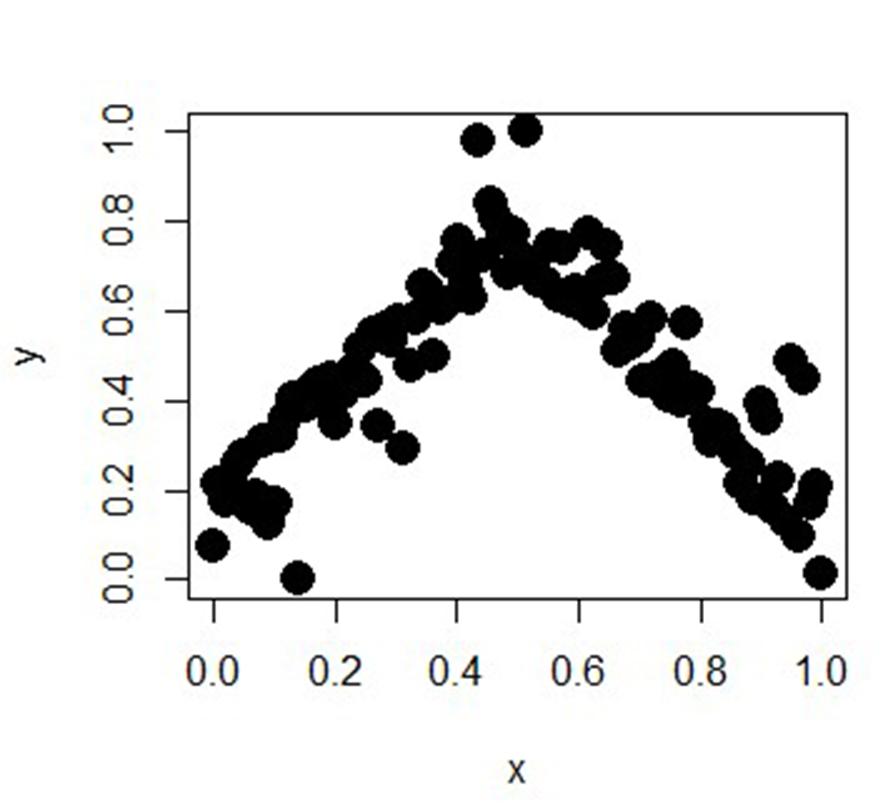
\includegraphics[width=0.5\linewidth]{ch-intro/figures/me1plot}
		\caption[A plot of data that exhibits a strong quadratic trend but fails common tests of dependence.]{A plot of data that exhibits a strong quadratic trend but fails common tests of dependence. The code for this analysis may be found in Appendix~\ref{sec:appendicies:me1plot}}
		\label{fig:intro:me1plot}
	\end{center}
\end{figure}
\section{Motivating example 2}
\label{sec:intro:me2}

In retrospect, it would have been simple to use polynomial regression or perform a non-linear dependency test in the previous motivating example. We argued that any unsuspecting analyst might have overlooked this since all the basic numerical methods were tried. Even if this is not true and the user did perform a non-linear correlation test, this does not necessitate that the results will be expected. We have developed another set of data to illustrate this point. Again, imagine that a data analyst cannot produce any plots in the analysis and is trying to determine if $x$ contains explanatory power of $y$. Again, we fit a linear regression. The ANOVA table returns a significance level of 0.1896, which indicates that it is insignificant. The next step is to check the significance of each term in the linear regression model. Both the $x$-intercept ($-0.131, p = 0.488$) and observed variable $x (-0.2699, p = 0.190)$ are not significantly different from zero. Finally, a hypothesis test is used to determine whether or not the residuals are normally-distributed. The large $p$-value (0.1632) of the Shapiro test suggests it is. Next, one can check the Pearson correlation of $x$ against $y$ (-0.189), but the $p$-value (0.1896) indicates that the two are uncorrelated (the correlation is not significantly different from zero). The final conclusion is that the data is uncorrelated. Again, the result is that the analyst scraps the regressions as they were ``uninteresting.''

Now assume that the data analyst is allowed to plot the data to verify their numerical solution. It is clear from Figure~\ref{fig:intro:me2plot} that the data exhibit a negative linear trend. The outliers near the top left and top right were enough to drag the correlation coefficient towards to 0. It is difficult to notice these outliers by printing the raw data or only using numerical methods. And with a larger multivariate dataset, it would be even more difficult.

\begin{figure}[htb]
	\begin{center}
		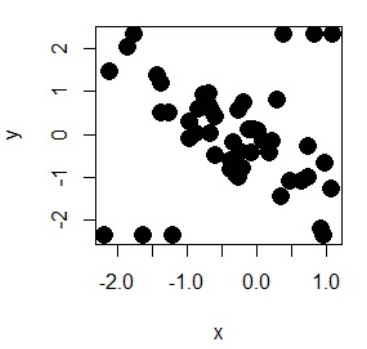
\includegraphics[width=0.5\linewidth]{ch-intro/figures/me2plot}
		\caption[A plot of data that exhibits a negative linear trend but fails the Pearson correlation test.]{A plot of data that exhibits a negative linear trend but fails the Pearson correlation test. The code for this analysis may be found in Appendix~\ref{sec:appendicies:me2plot}}
		\label{fig:intro:me2plot}
	\end{center}
\end{figure}

Notice that the analyst used a common test of linear correlation, and the data is clearly linear. The test, however, did not indicate that there was a significant relationship among the two variables; it was only after the data was plotted that this relationship was immediately noticed. Indeed, the data used in these examples was purposefully constructed to be dependent but bypass common tests for dependency. However, if it is possible to construct datasets in one-dimension that evade commonly-used numerical methods, it is believable that it is even easier to construct analogous datasets in higher dimensions.

\section{Solution overview}
\label{sec:intro:solution}

In this work, we tackle the problem by developing a sophisticated visualization system (abbreviated VS) to explore the data and numerical model in a different way. Specifically, we focus on two aspects of the VS that addresses the two problems raised in Section~\ref{sec:intro:problem}: (1) the procedure of sorting through plots is efficiently automated by learning the user's interests, and (2) the procedure of comparing the numerical and visual output is also automated. This allows the system to find visually interesting relationships that the numerical model may have missed and/or toss out relationships which turn out to be uninteresting. Furthermore, this allows future analysts to combine visual feedback with the numerical feedback from estimators to make better decisions during data analysis and provide clear justification of their decisions.
\section{Correlation graphs}
\label{sec:intro:correlation}

Independence graphs are one way to discover the dependency structure among
different stocks whose prices may be represented as random variables following
some distribution. The importance of independence among assets is explained 
later in Section~\ref{sec:intro:finance}.

Let $G=(V,E)$ be an undirected graph formed from the population 
$X$. Given that there are $d$ observations of $n$ variables in $X$, 
$G$ has vertices $|V| = n$ and edges $E_{i,j}\in\{0,1\}$. 
$E_{i,j}=1$ when there is an edge between $V_i$ and $V_j$, and 0 otherwise. 
Edges are determined with the following heuristic: \\

\begin{algorithm}
	$E_{i,j} = 0$ for $i\neq j$ if and only if $X_i \perp X_j$ (the two 
	variables are independent)
\end{algorithm}

Unfortunately, independence graphs are difficult to implement in practice since 
independence is determined by the true joint distributions of all $n$ variables 
in $X$, which is difficult to determine. However, the independence graph 
$G$ may be estimated by the sample correlation graph 
$\hat{G}=(V,\hat{E})$. While it is true that non-correlation does 
not always imply independence, it is a useful estimate for \textit{some} form 
of independence between the two variables. 
It is important to be careful about the terminology usage. Here, 
``correlation'' is used to refer to \textit{any form} of pair-wise dependence. 

There are two main methods to estimate correlation; the first and most common 
is via \textbf{numerical correlation}. 
By ``numerical correlation'', we do not mean the traditional mathematical 
interpretation of ``Pearson's correlation'' but, instead, anything which 
involves explicitly computing an estimate of the correlation e.g. Pearson's, 
Spearman's, and various other correlation metrics which are described later in 
this section. 
Let $\hat{G}^{\text{num}}$ be the numerical graph. $\hat{G}^{\text{num}}$ can 
be drawn from a matrix of $p$-values (for each correlation) $P$ where 
$P_{i,j}=p(V_i,V_j)$ with the following heuristic:\\

\begin{algorithm}
	$E_{i,j} = 1$ for $i\neq j$ if $P_{i,j} \leq p$ where $p$ is the $p$-value 
	for the desired confidence level
\end{algorithm}

Alternatively and more simplistically, this numerical correlation graph can be 
drawn from a correlation matrix $\hat{\Sigma}$ where 
$\hat{\Sigma}_{i,j}=\hat{\rho}(V_i,V_j)$ (some sample correlation coefficient) 
with the following heuristic:\\

\begin{algorithm}
	$E_{i,j} = 1$ for $i\neq j$ if $|\hat{\Sigma}_{i,j}| \geq \lambda$ where 
	$\lambda$ is the desired threshold value for a ``significant'' correlation 
	(e.g. $\lambda = 0.75$)
\end{algorithm}

\noindent We implement this latter approach when drawing correlation 
graphs in Chapter~\ref{ch:usage}'s application.

The second method is via \textbf{visual correlation}. Visual correlation can be 
thought of as ``pairs of variables that marginally appear dependent''. 
Subsequently, the visual graph $\hat{G}^{\text{vis}}$ can be drawn with the 
following heuristic:\\

\begin{algorithm}
	$E_{i,j} = 1$ for $i\neq j$ if the scatterplot of pair $(X_i, X_j)$ 
	contains a distinct trend
\end{algorithm}

This definition of ``visual correlation'' is, admittedly, subjective by nature 
and, as a consequence, slightly vague. Traditionally, 
numerical correlation is used over visual correlation because it's more 
objective. However, visual correlation is still necessary in conjunction with 
numerical correlation. Consider if the joint distributions of the variables 
changed over time or if there were outliers as in the example of 
Section~\ref{sec:intro:problem}. While the dependency of the variables could 
not be captured by standard correlation metrics, we have a notion of the visual 
correlation between them. But because visual interpretations are subjective and 
dependent on how the data is plotted, numerical correlation is still useful. 
The two views on estimating the population correlation do not have to be 
mutually exclusive and actually supplement each other's faults instead.
What follows is an overview of common numerical methods 
to estimate the correlation between two random variables. It will become clear 
that the numerical correlation metrics below are sensitive in some way or 
another, further emphasizing the need for both methodologies.

\subsection{Pearson's correlation}

Pearson's correlation measures the linear dependence among two random variables
$X$ and $Y$. In a population, the Pearson correlation is given by
$$\rho_{X,Y}=\frac{\Cov(X,Y)}{\sigma_X \sigma_Y} =
\frac{\E(XY)-\E(X)\E(Y)}{\sqrt{\E(X^2)-\E(X)^2} \sqrt{\E(Y^2)-\E(Y)^2}}$$ 

The quantity above is typically unknown in practice since the expectation 
requires knowing the true joint distribution of $X$ and $Y$. Instead, it is 
typically estimated by the sample Pearson correlation. Given data with $n$ 
samples, the sample expectation is given by the formula  
$\E(X)=\frac{1}{n}\sum\limits_{i=1}^{n}x_i$. 
By substituting into the formulation above and multiplying by $n^2/n^2$, we can 
estimate the sample Pearson correlation with the following:
$$\hat{\rho}_{x,y}^\text{Pear}=
\frac{n \sum\limits_{i=1}^{n} x_i y_i - \sum\limits_{i=1}^{n} x_i
	\sum\limits_{i=1}^{n} y_i}
{\sqrt{n\sum\limits_{i=1}^{n} x_i^2-\left(\sum\limits_{i=1}^{n} x_i\right)^2} 
	\sqrt{n\sum\limits_{i=1}^{n} y_i^2-\left(\sum\limits_{i=1}^{n} y_i\right)^2}}$$ 

\noindent such that $-1 \leq \hat{\rho}_{x,y}^\text{Pear} \leq 1$. With perfect 
positive and negative linear 
dependence respectively, $\hat{\rho}_{x,y}^\text{Pear}=\pm1$.
It is important to note that $\hat{\rho}_{x,y}^\text{Pear}=0$ does not 
necessarily indicate independence, though it is an indication of 
\textbf{linear} independence.

\subsection{Spearman's correlation}

Spearman's correlation is more broad than Pearson's; it measures monotonic
dependence among two random variables $X$ and $Y$. Monotonic functions are
either strictly increasing or decreasing; while linear functions are monotonic,
monotonic functions are not necessarily linear. Subsequently, Spearman's
correlations may also capture non-linear dependencies. Spearman's correlation is
computed by computing the Pearson's correlation among ``ranked variables''. Each
sample observation $x_i$ of $X$ is ranked from 1 to $n$ based on its position
relative to $x_j, j\in\{1,...,n\}\backslash{i}$. The ranking is also computed
for all observations of $Y$. We then define the difference of a sample
$(x_i,y_i)$ as $d_i=x_i-y_i$ and compute the sample Spearman's correlation as
$$\hat{\rho}_{x,y}^{\text{Spear}}=
1-\frac{6 \sum\limits_{i=1}^{n}d_i^2}{n(n^2-1)}$$

\noindent such that $-1 \leq \hat{\rho}_{x,y}^{\text{Spear}} \leq 1$. With 
perfect increasing and decreasing monotonic dependence respectively,
$\hat{\rho}_{x,y}^{\text{Spear}} = \pm1$. Again, it is important to note that 
$\hat{\rho}_{x,y}^{\text{Spear}}=0$ does not necessarily indicate 
independence, though it is an indication of \textbf{monotonic} independence.

\subsection{Kendall's tau}

Similar to Spearman's correlation, Kendall's tau is another method of
identifying monotonic dependence among two random $X$ and $Y$ as it also
computes correlation among ranked variables. However, it does not utilize the
difference among a single sample. Instead, it compares pairs of samples among
each other. For $i\not=j$, $(x_i,y_i)$ and $(x_j,y_j)$ are defined as
``concordant'' if the ranks of both elements agree i.e. $x_i > x_j$ and $y_i >
y_j$ or $x_i < x_j$ and $y_i < y_j$. Pairs are defined as ``discordant'' if the
ranks of both elements disagree i.e. $x_i > x_j$ and $y_i < y_j$ or $x_i < x_j$
and $y_i > y_j$. In the case where ranks of either element are equal, the pair
is ignored. Let $c=$ the number of concordant pairs and $d=$ the number of
discordant pairs. Then the sample Kendall's tau is computed as 
$$\hat{\rho}_{x,y}^{\text{Kend}}=\frac{c-d}{n(n-1)/2}$$

\noindent such that $-1 \leq \hat{\rho}_{x,y}^{\text{Kend}} \leq 1$. 
Kendall's tau is less sensitive to errors in the data as its correlation is
based on sample pairs rather than deviations within an observation, though the
resulting values tend to result in the same interpretations. As with Spearman's
correlation, $\hat{\rho}_{x,y}^{\text{Kend}}=\pm1$ with perfect increasing 
and decreasing monotonic dependence respectively. Furthermore, 
$\hat{\rho}_{x,y}^{\text{Kend}}=0$ does not necessarily indicate
independence, though it is an indication of \textbf{monotonic} independence.

\subsection{Distance correlation}

While the aforementioned correlation metrics are well-known and commonly used, 
they are constrained to monotonic functions. Distance correlation was first 
proposed in 2007 as a way to further test for non-monotone dependence between 
$X$ and $Y$~\cite{szekely2007}. The distance correlation is a function of the 
distance covariance and distance variance of $X$ and $Y$. We define the 
$n\times n$ matrices $a$ and $b$ as the distance matrices of $X$ and $Y$ 
respectively. The elements $a_{k,l}$ and $b_{k,l}$ are respectively defined as 
$||X_k-X_l||$ and $||Y_k-Y_l||$ for all $k,l=1,2,...,n$ where $||z||$ is the 
Euclidean norm $\sqrt{z_1^2+...+z_n^2}$. Then we define the sample distance 
covariance and sample distance variance as 

\tablespacing
\begin{itemize}
	\item $\mathrm{dCov}(X,Y) = \sqrt{\frac{1}{n^2} \sum\limits_{k=1}^{n} 
	\sum\limits_{l=1}^{n} A_{k,l} B_{k,l}}$
	\item $\mathrm{dVar}(X) = \mathrm{dCov}(X,Y)$
	\item $\mathrm{dVar}(Y) = \mathrm{dCov}(Y,Y)$
\end{itemize}
\bodyspacing

\noindent where $A_{k,l}=a_{k,l}-\bar{a}_{k,}-\bar{a}_{,l}+\bar{a}$ and 
$\bar{a}_{k,}$ is the $k$th row mean of $a$, $\bar{a}_{,l}$ is the $l$th column 
mean of $a$, and $\bar{a}$ is grand mean of $a$. 
Similarly, $B_{k,l}=b_{k,l}-\bar{b}_{k,}-\bar{b}_{,l}+\bar{b}$ and 
$\bar{b}_{k,}$ is the $k$th row mean of $b$, $\bar{b}_{,l}$ is the $l$th column 
mean of $b$, and $\bar{b}$ is grand mean of $b$. The sample distance 
correlation is then defined as
$$\hat{\rho}_{x,y}^{\text{Dist}}=\frac{\mathrm{dCov}(X,Y)}
{\sqrt{\mathrm{dVar}(X)\mathrm{dVar}(Y)}}$$

\noindent with the variance and covariance values given earlier such that 
$0 \leq \hat{\rho}_{x,y}^{\text{(Dist)}} \leq 1$. As before, 
$\hat{\rho}_{x,y}^{\text{(Dist)}}=1$ indicates perfect dependence. 
Like the other correlation metrics, $\hat{\rho}_{x,y}^{\text{Dist}}=0$ implies 
some form of independence. 
However, the interpretation of $\hat{\rho}_{x,y}^{\text{Dist}}=0$ is
interesting in the sense that its corresponding population correlation metric
$\rho_{x,y}^{\text{Dist}}$ has two important properties not seen in the other 
population metrics~\cite{szekely2007}: 

\tablespacing
\begin{enumerate}
	\item $X$ and $Y$ may be of different dimensions.
	\item$\rho_{x,y}^{\text{Dist}}=0$ if and only if $X$ and $Y$ are 
	independent.
\end{enumerate}
\bodyspacing



\section{Portfolio management}
\label{sec:intro:finance}

An important application of correlation graphs is in modeling the dependencies 
among equities. Determining the relationship among various stocks is 
especially useful when managing portfolios. One such methodology is the ``buy 
and hold'' tactic where an investor selects a portfolio of stocks and never 
rebalances. The idea is to select diversified stocks with low correlation and 
positive drift such that losses are offset by gains, and the portfolio gains on 
average. As such, portfolio selection is the main decision-making component of 
the ``buy and hold'' method. This strategy is especially useful when 
transaction costs are high as fees are prohibitive to rebalancing gains. 

In a world with low transaction costs, however, there is more to be gained 
(less to be lost, alternatively) by frequently rebalancing the portfolio rather 
than holding. The concept for rebalancing is similar to that of ``buy and 
hold'', though there are some key differences. Another component for successful 
rebalancing gains is for the stock returns to be relatively 
independent~\cite{liuh2016}. Thus, when one stock goes down, the others do not 
fall with it; with perfect independence, rebalancing gains become a function of 
the volatility of the stocks rather than of stock returns. Independence is 
further important because frequent asset trading may move the market and lead 
to unexpected price swings. With independent stocks, the price risk associated 
with rebalancing is minimized. In summary, rebalancing gains are best suited to 
markets with low correlation, independent returns, and high 
volatility~\cite{liuh2016}. 

In this thesis, we focus on the problem of portfolio selection and, 
specifically, its application to the ``buy and hold'' strategy. However, 
portfolio selection is still a component of the rebalancing strategy, so our 
findings and proposed procedures may be further extended to portfolio 
management techniques.
A detailed application may be found in Chapter~\ref{ch:usage} where
a stock selection methodology for correlation graphs is also proposed.

We acknowledge that non-correlation does not necessitate independence, but it 
is still a useful proxy for independence.
Again, it must be noted that numerical correlation alone cannot capture the 
full complexity of these financial applications; in fact, cases such as that of 
Figure~\ref{fig:intro:meplot} (right) reflect the limitations of correlation 
coefficients and reinforce the importance of visualization in aiding with the 
selection of numerical metrics. An unassuming 
analyst might select the stocks (variables) from Table~\ref{tab:intro:me}, 
Dataset 2, because their numerical correlation is not significantly different 
from zero. But, it turns out that the stocks are highly correlated, and this is 
only clear when looking for visual correlation. However, numerical correlation 
is still an important component of portfolio management in theory and in 
practice. 
As such, an important goal of this thesis is to not only develop a 
solution to the problem of high-dimensional visualization described in 
Section~\ref{sec:intro:problem} but to also consider the reason we are 
interested in visualization in the first place. As noted earlier, plotting is 
an incredibly useful tool to check numerical methods. Thus, we will also 
develop a method to quickly check the output from numerical methods with an 
analyst's own concepts of visual dependence, allowing the analyst to select the 
numerical method most suited to their application (numerical correlation graphs 
and portfolio selection, in this case). 
What follows is a road map of the high-dimensional visualization solution that 
is developed further in this thesis with 
Chapters~\ref{ch:visualizer},~\ref{ch:al}, and~\ref{ch:gc}.
% summary of following chapters

\chapter{Visualization System \label{ch:visualizer}}

Regardless of whether high dimensional data visualization methods are
computationally heavy or interaction heavy, user interactivity is a critical
component of high dimensional visualization analysis; it is simply a
question of what degree~\cite{lius2016}. It is not enough to simply have user 
interaction, however. Given $d$ variables, there are a total of $d\choose 2$ 
possible scatter plots of the data. This blows up almost quadratically as $d$ 
increases, which is infeasible for the analyst to sort through in any 
reasonable amount of time. Subsequently, automation is another necessary 
element in the task of visualizing high dimensional datasets.

We develop a system that first learns what visual patterns the data analyst 
finds promising, querying the user where the decision boundary is ambiguous. It 
then automatically iterates through thousands
of possible plots and returns an adjacency matrix that captures the 
classifications of variable pairs. The VS may then return several plots for the 
user, perform line-up tests to refine the tree~\ref{sec:futurework:lineup}, or 
compare the visual graph with a numerical graph of the user's choice. This 
allows users to compare and contrast visual feedback with numerical
algorithms for improved model selection. Figure~\ref{fig:visualizer:vs} 
is a visual summarization of the system.
       
\begin{figure}[htb]
	\begin{center}
		
\includegraphics[width=1\linewidth]{ch-visualizer/figures/vs}
		\caption[Broad overview of the visualization system.]{Broad overview of 
		the visualization system.}
		\label{fig:visualizer:vs}
	\end{center}
\end{figure}

Section~\ref{sec:visualizer:scatterplot} describes characteristics of an 
interesting plot; mindfulness and incorporation of these ideas in the VS 
facilitates improves user accuracy in stage 1 . 
Sections~\ref{sec:visualizer:al} and ~\ref{sec:visualizer:plotgeneration} 
provide a brief overview of stage 1 and stage 2 respectively (see 
Figure~\ref{fig:visualizer:vs}) while 
Section~\ref{sec:visualizer:focus} describes the focus of the rest of the work 
which respond to the problems posed in Section~\ref{sec:intro:problem}.

\section{Scatterplot characterization}
\label{sec:visualizer:scatterplot}

\subsection{Characteristics of a ``good'' plot}
\label{sec:visualizer:scatterplot:goodplot}

The simplest scatter plot is one without any transformations on the data. This,
however, may not be the best way to ascertain independence for the user. This
notion is illustrated in Figure~\ref{fig:visualizer:cdf}. The left plot appears
to be independent as it's a cluster of points near the origin, but it's not
entirely clear due to the multitude of stray points outside of $y\in (-2,2)$ 
and $x\in(-1.5,1.5)$. By looking at the outliers, it could also be argued that 
there is some dependency. However, applying the CDF in both directions creates 
a plot distributed on (0,1). This transformation is non-destructive and 
preserves dependency in the data if it exists. The data is clearly independent 
as the points appear to be uniformly distributed within the box.

\begin{figure}[htb]
	\begin{center}
		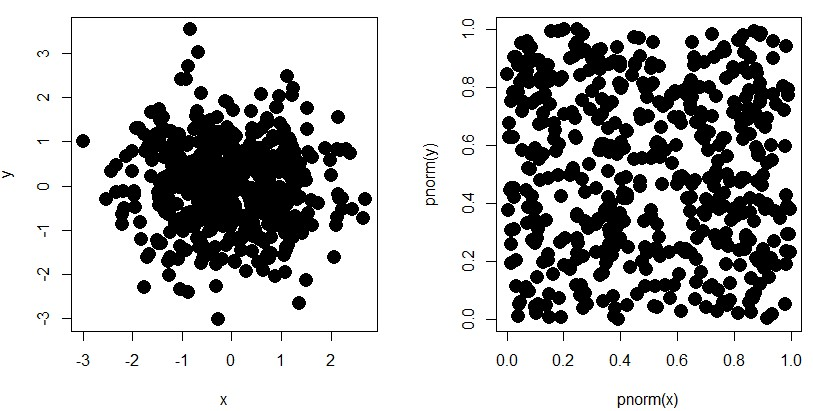
\includegraphics[width=0.75\linewidth]{ch-visualizer/figures/cdf}
		\caption[A plot of $y$ against $x$ after the CDF is applied in both
		directions.]{A plot of $y$ against $x$ with no transformation (left) 
		and after
			the CDF is applied in both directions (right). The code for this 
			example may be
			found in Appendix~\ref{sec:appendicies:cdf}}
		\label{fig:visualizer:cdf}
	\end{center}
\end{figure}

Restricting the scatter plot to a unit box allows analyst's visual systems to 
focus on locations where there is low spatial frequency, which is ideal for 
detecting dependence~\cite{hofert2016}. The effects of this concept can be 
progressively observed from left to right in 
Figure~\ref{fig:visualizer:hofertoldford} below.

\begin{figure}[htb]
	\begin{center}
		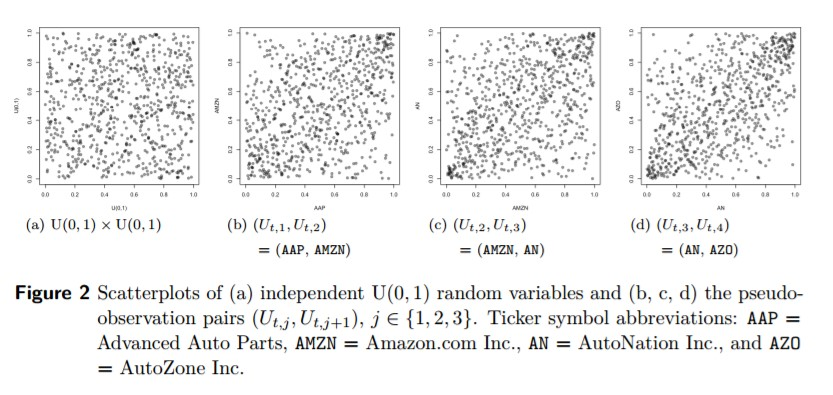
\includegraphics[width=1\linewidth]{ch-visualizer/figures/hofertoldford}
		\caption[Transformed scatter plots of independent $U(0,1)$ random 
		variables and pseudo-observation pairs $(U_{j},U_{j+1}),j\in 
		\{1,2,3\}$ which are more correlated the larger $j$ is.]{\textit{(a):} 
		Transformed scatter plots of independent $U(0,1)$ random variables. 
		\textit{(b,c,d):} Transformed scatter plots of the pseudo-observation 
		pairs $(U_{j},U_{j+1}),j\in \{1,2,3\}$. The variables are clearly more 
		correlated as $j$ increases; this trend can easily be observed due to 
		the nature of the unit box. Ticker abbreviations: 
		AAP = Advanced Auto Parts ($U_1$), AMZN = Amazon.com Inc. ($U_2$), 
		AN = AutoNation Inc. ($U_3$), AZO = AutoZone Inc. ($U_4$).
		Figure from Hofert and Oldford 2016 with slight 
		modifications~\cite{hofert2016}}
		\label{fig:visualizer:hofertoldford}
	\end{center}
\end{figure}

\subsection{Feature extraction from plot}
\label{sec:visualizer:scatterplot:features}

In order for the active learning classifier to properly understand and classify 
all $n \choose 2$ scatter plots in stage 1 and 2
(Sections~\ref{sec:visualizer:al} and~\ref{sec:visualizer:plotgeneration}), 
characteristic features must be extracted from each pairwise scatter plot. The 
more useful criteria there are, the more sophisticated the classification will 
be.

\subsubsection{Numerical features}

Our goal is to quantify various features of a scatter plot for the computer, 
and that does include numerical features. The following features are currently 
implemented in the VS: 

\tablespacing
\begin{itemize}
	\item \textbf{Correlation coefficients and their $p$-values:} Examples 
	include Pearson's, Spearman's, Kendall's, and distance correlation. See 
	Section~\ref{sec:intro:correlation} for more details on the various types 
	of coefficients.
	\item \textbf{Kullback-Leibler divergence criterion:}
	\item \textbf{Chi-square test of independence and its $p$-value:}
\end{itemize}
\bodyspacing 

\subsubsection{Visual features}

What is more challenging is to find a way to quantify the visual features of 
scatter plots. This may be done by looking for concentration of points in 
various spaces of the plot domain. The following features are currently 
implemented in the VS: 

\tablespacing
\begin{itemize}
	\item \textbf{Middle box criterion:} The percentage of points near the 
	center of the plot
	\item \textbf{LR criterion:} The percentage of points that lie above and 
	below the linear regression line
	\item \textbf{Clustering criterion:} The percentage quantile of the ratio 
	between the largest and next-largest distance
	\item \textbf{Visual trend criterion:} This is computed as 
	max(PosTrendCriterion, NegTrendCriterion). The positive trend criterion 
	(PosTrendCriterion) is computed from the percentage of points in the bottom 
	left and upper right while the negative trend criterion (NegTrendCriterion) 
	is computed from the percentage of points in the upper left and 
	bottom right. A higher visual trend criterion value suggests a greater 
	visual trend. 
\end{itemize}
\bodyspacing
\section{Active learning (Stage 1)}
\label{sec:visualizer:al}

The main goal of stage 1 is to learn the user's interests. This requires the 
system to select (``query'') data (which are $n$ characterizations of $d\choose 
2$ plots in the case of the VS as described in 
Section~\ref{sec:visualizer:scatterplot:features}) for the analyst (the 
``oracle'') to label (classify). The learner may then utilize a classification 
model (LDA, QDA, naive bayes, decision tree, random forest, logistic 
regression, etc.) that trains on labeled data to ``learn'' user interests. The 
user's interests are encoded in a classifier (some instance of the 
classification model) that is applied to automatically label the rest of the 
data (For more on the 
semantic differences between ``classification model'' and ``classifier'', see 
Figure~\ref{fig:visualizer:al:tree}). As such, it is important to make the 
process as efficient as possible to avoid redundancy for the end user. There 
are various methods that may be used for querying in stage 
1~\cite{dasgupta2011}:

\tablespacing
\begin{itemize}
	\item \textbf{Supervised learner}: This learner queries a single, random 
	subset of all unlabeled data. It ignores the rest of the data when refining 
	the classifier
	\item \textbf{Semisupervised learner}: Similar to a supervised learner, a 
	semisupervised learner queries a single, random subset of all 
	unlabeled data but proceeds to utilize the remaining unlabeled data to 
	better inform the final classifier
	\item \textbf{Active learner}: An active learner selects its queries in a 
	non-random, intelligent manner to reduce the hypothesis space $\mathcal{H}$ 
	of all possible classifiers that may explain the data.
\end{itemize}
\bodyspacing

It has been 
shown that when a learning algorithm is allowed to choose its next query, it 
performs better with less training; as such, we choose to utilize active 
learning to select the plots to be queried by the oracle in stage 
1~\cite{settles2010}. Chapter~\ref{ch:al} goes into detail on different active 
learning methodologies as this section is primarily focused on its role in the 
system.

\begin{figure}[htb]
	\begin{center}
		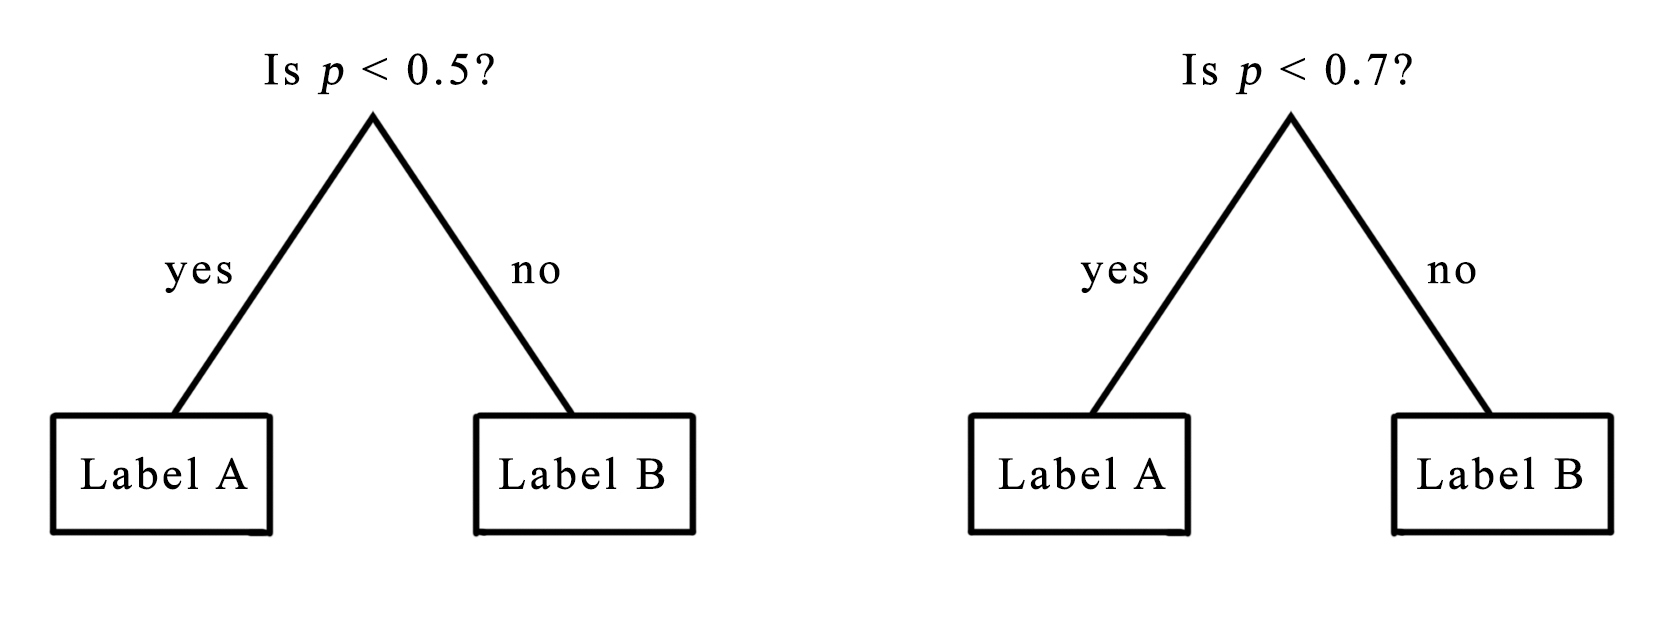
\includegraphics[width=0.75\linewidth]{ch-visualizer/figures/tree}
		\caption[Classifiers and classification models]{Although both figures 
		on the left and right are slightly different classifiers, they 
		are both instances of (extremely simple) decision trees.}
		\label{fig:visualizer:al:tree}
	\end{center}
\end{figure}

\subsection{Initialization of active learner}
\label{sec:visualizer:al:initialization}

It is problematic to start from scratch; how does the system determine
the best first point of ambiguity when it knows nothing (the hypothesis space is
everything)? A classic method is to simply select $k$ random data instances for 
the user to label. As initialization is not the focus of this work, the VS 
currently utilizes this methodology.

Alternatively, we can exploit the fact that the
user is already providing a numerical model that they believe to be a good
representation of the data which they would like the visualization system to
check visually. Given this data, the system builds a decision tree that utilizes
the various properties of the plots to determine whether one is interesting or
uninteresting. Doing so greatly narrows the hypothesis space and makes it easier
to determine points of ambiguity. However, to reconcile with the fact that the
user wishes to check the numerical model and may not necessarily believe it is a
good representation of fit, the learner must check whether the initial decision
tree is a proper fit (This may be achieved with line-up tests, which are 
described briefly in Section ~\ref{sec:futurework:lineup}). As the user then 
proceeds to label various conditional
plots as ``interesting'' or ``not interesting,'' the classifier learns the
user’s interest and continues to evolve. This models plot characteristics that
the user found interesting to study.

\subsection{Decision tree classification of user interests}
\label{sec:visualizer:al:tree}

Post-initialization, the active learner cleverly queries vital plots so that 
the system can best learn the user’s interests. The system first determines 
which features it is uncertain about classifying and then returns a plot 
matching those characteristics to the user. This allows the system to utilize 
its classification model of choice to build a better classifier more 
efficiently. It is important to distinguish between the active learner, which 
selects the next queries from the pool of unlabeled data, and the
classification model, which trains on labeled data to ``learn'' user interests 
and classify (predict) the remaining unlabeled data. 

A random forest is one model for classifying and labeling data (features of 
plots, in the case of the visualization system). In a random forest, various 
decision trees are constructed from random samples of the data. Each classifier 
has a vote of weight one for each unlabeled data, and the forest is aggregated 
by majority vote. It is easily presented to the 
analyst in the form of a decision tree, which aids in user 
interpretability of the system output. As such, the VS sets the choice of 
classification model to random forest by default.

\section{Automated plot generation (Stage 2)}
\label{sec:visualizer:plotgeneration}

\subsection{User interaction with active learning output}
\label{sec:visualizer:plotgeneration:user}

The system has now learned which of the unlabeled plots 
may be of interest to the user. The final learned classifier is used to fit the 
rest of the $d \choose 2$ unlabeled scatterplots, and a visual graph $G=(V,E)$ 
may be built from these labels with the following heuristic where $i,j \in 
\{1,...,d\}$:

\begin{algorithm}
	If label($i,j)>0$ (i.e. ``interesting'' instead of ``uninteresting''), draw 
	edge $E_{i,j}$
\end{algorithm}

Furthermore, the VS may provide a visualization of the resulting classifier 
itself such as the decision tree itself. The active learning output may be 
visualized as a heat map. A 
classic heat map represents each pair of variables as colors from a bivariate 
spectrum. Heat maps are difficult to interpret as it is one-dimensional; each 
end of the color spectrum represents minimum and maximum values respectively. 
It is unclear what the max or the min is as it depends on the domain of the 
whatever the heat map is plotting; as such, the minimum may not necessarily be 
negative while the maximum may not necessarily be positive. Furthermore, the 
subtle variations in hue between colors make it difficult to compare relative 
ranking among different pairs for colors that are similar. Buja \textit{et al.} 
propose an alternate, clearer method of visualizing the heat map, termed the 
``association navigator''~\cite{buja2016}. The association navigator is 
two-dimensional: the size of each color corresponds to its value while the 
color 
represents a positive or negative value~\cite{buja2016}. As such, the 
association navigator only utilizes two colors rather than a spectrum of 
colors, making it simple to distinguish between the two. By simplifying the 
color scheme and adding the dimension of size, the association navigator makes 
it much easier to interpret and compare different pairs of data at a glance. 
The stark difference between a traditional heatmap and the association 
navigator when applied to the same dataset may be seen in 
Figure~\ref{fig:visualizer:heatmap}. The VS provides both options, allowing the 
analyst to select whichever is easier to for them to interpret. 
With these visualizations of the active learning output, the user should be 
able to understand his/her own interests. 

\begin{figure}[htb]
	\begin{center}
		
\includegraphics[width=1\linewidth]{ch-visualizer/figures/vs}
		\caption[Heatmap versus association navigator]{Heatmap versus 
		association navigator example.}
		\label{fig:visualizer:heatmap}
	\end{center}
\end{figure}

\subsection{System output}
\label{sec:visualizer:plotgeneration:output}

There are three options at the end of stage 2. Two of them are concrete outputs 
that may be easily used in an analyst's final report, and the third is a 
refinement of the active learning component in stage 1.

\tablespacing
\begin{itemize}
	\item \textbf{Automatic plot generation:} The VS compiles a selection of 
	the most interesting and non-interesting plots along with their 
	associated transformation variables.
	\item \textbf{Graph comparison:} The VS accepts a numeric graph (For 
	example, a correlation graph $G^{\text{num}}$ generated with numerical 
	correlation 
	coefficients as described in Section~\ref{sec:intro:correlation}) and 
	measures the difference between the numeric graph $G^{\text{num}}$ and 
	visual graph $G$ (the active learning output). 
	Details on different graph comparison methods may be found in 
	Chapter~\ref{ch:gc}.
	\item \textbf{Lineup test:} In the event that the classifier is not a 
	satisfactory representation of the analyst's interests, the VS may utilize 
	lineup tests to help determine where to query from further. For more 
	details on this methodology, see Section~\ref{sec:futurework:lineup}.
\end{itemize}
\bodyspacing

With the focus on correlation graphs in this work, graph comparison is the most 
useful output from the visualization system. As such, it is one of our primary 
VS focuses. The next section provides a roadmap for the rest of this work, 
which goes into detail on two aspects of the VS. 
\section{Specific focus: AL and GC}
\label{sec:visualizer:focus}

The active learning component is the bread and butter of the visualization 
system and forms the first stage of the system. Furthermore, it solves for the 
tedious nature of classifying $d \choose 2$ plots in high-dimensional 
visualization , which was first brought up in Section~\ref{sec:intro:problem}. 
The second issue with high-dimensional visualization is the verification of the 
numerical results against the visual result. This is a question of the VS 
output, and graph comparison is a solution to this problem that is both 
informative to the analyst and further useful in the case of correlation 
graphs, which we are interested in for their financial applications. As such, 
the primary focus of this work that follows are active learning methods 
(Chapter~\ref{ch:al}) and graph comparison methods (Chapter~\ref{ch:gc}). These 
methods are applied to the current iteration of the VS, which is then utilized 
in conjugation with numerical correlation graphs to perform stock selection.

It should be noted that the VS is a large project and may certainly be further 
refined despite the work that we do to refine two major components of the 
system. Ideas for future extensions of the VS may be found in 
Section~\ref{sec:futurework}. There are several recommendations for 
improvements that can be made to different aspects of the system which are not 
the focus on this work.

\chapter{Active learning \label{ch:al}}

Active learning is a subset of machine learning wherein an algorithm is 
``trained'' on labeled data instances in order to learn from and make 
predictions on the data.  Consider a large set of unlabeled data $X$ with a 
hidden label from a finite set $Y$ that can be queried from some human 
``oracle''; we would like to learn a good classifier of the data, some mapping 
$h: X \rightarrow Y$ from the set $\mathcal{H}$ without making too many 
queries~\cite{dasgupta2011}. Active learning is the process of intelligently 
selecting the queries (a constrained resource) to learn as much as possible. 
When a learning algorithm is allowed to choose its next query, it performs 
better with less training~\cite{settles2010}. To put it more concretely, the 
error (a measurement of the difference between the predicted labels and the 
``true'' labels) converges to zero faster. This property is especially 
desirable when labeled data are difficult, time-consuming, or computationally 
expensive to obtain. Stage 1 of the VS (Section~\ref{sec:visualizer:al}) is 
one such classification task where $Y\in\{$interesting, non-interesting$\}$. 
Classification and filtering tasks are both tedious and redundant, which 
necessitates intelligent selection of queries~\cite{settles2010}. What follows 
is an active learning literature review in Section~\ref{sec:al:litreview}, an 
overview of active learning methods and their algorithms in 
Section~\ref{sec:al:methods}, and a simulation study in 
Section~\ref{sec:al:simulations} to determine the method that is best-suited 
for usage with the VS in Chapter~\ref{ch:usage}'s equity application.

\section{Literature review}
\label{sec:al:litreview}

It is important to consider the main framework in which the learning algorithm 
selects a query from unlabeled data. There are three different 
scenarios in which the learner may request queries as described by 
Settles~\cite{settles2010}:
 
\tablespacing
\begin{enumerate}
	\item \textbf{Membership query synthesis}: The learner may select a query 
	from any unlabeled samples in $X$.
	\item \textbf{Stream-based selective sampling}: An unlabeled sample is 
	randomly selected from $X$, and the learner decides whether to query or not.
	\item \textbf{Pool-based sampling}: $k$ unlabeled samples are randomly 
	selected from $X$, and the learner picks one to query.
\end{enumerate}
\bodyspacing

\noindent While the methods above may apply to many different active learning 
environments, the specific situation for the VS is \textit{pool-based selective 
sampling}. Because it is computationally expensive to extract features from 
every single $n\choose2$ plot (see 
Section~\ref{sec:visualizer:scatterplot:features}), membership query synthesis 
is not an option. While stream-based selective sampling may work, it has a 
similar problem because there are no constraints
on the number of samples that the algorithm may choose to discard. 

The next problem, then, is to determine the informativeness of unlabeled 
instances that are presented by the situations above. This is the crux of 
active learning as it allows for intelligent selection of queries.
Dasgupta identifies two different approaches to active learning that are 
fundamental to the process of query selection~\cite{dasgupta2011}: 

\tablespacing
\begin{enumerate}
	\item \textbf{Efficient search through hypothesis space $\mathcal{H}$}: 
	The idea is to select a query that shrinks $\mathcal{H}_t$, the set of all 
	possible classifiers at time $t$ that explain the labeled data, as much as 
	possible. 
	\item \textbf{Exploiting cluster structure in data}: 
	The idea is to cluster the data and select queries based on cluster 
	structure (i.e. query from each cluster). While clusters may be split over 
	time if they are discovered to be non-homogenous, a learner may leverage 
	situations where clusters are fairly homogeneous in order to classify 
	points by propagating a node's label to its neighbors. 
\end{enumerate}
\bodyspacing

\noindent Uncertainty sampling, query by committee, and query by bagging are 
active learning algorithms that are a form of the aforementioned efficient 
search through the hypothesis space. These algorithms may be found in 
Sections~\ref{sec:al:methods:uncertainty} to~\ref{sec:al:methods:bagging} 
respectively. We also present a clustering partitioning algorithm in 
Section~\ref{sec:al:methods:clustering} that seeks to exploit the clustering  
structure in the data.

\section{Overview of active learning methods}
\label{sec:al:methods}

In this section, we present algorithms for specific active learning methods and 
a reference to its implementation in the appendix. The 
\texttt{activelearning} package by \texttt{ramhiser}~\cite{ramhiser2015} has 
adapted much of the methods reviewed in Settles' paper~\cite{settles2010}. As 
such, most of the implementation code has been adapted and reworked (with 
substantial components written from scratch) from the 
\texttt{activelearning} package, which is too general for our purposes.

\subsection{Uncertainty sampling}
\label{sec:al:methods:uncertainty} 

In uncertainty sampling, the active learner selects the query $q$ that it is 
most uncertain on how to label; in other words, the algorithm queries the label 
that has the highest posterior probability~\cite{lewis1994}. With binary 
classification as is the case with the VS (either ``visually correlated'' or 
``not visually correlated''), this reduces to the case of querying the instance 
whose posterior probability of being ``visually correlated'' is closest to 
0.5~\cite{lewis1994}. While the uncertainty sampling algorithm presented in 
Algorithm~\ref{alg:al:methods:uncertainty} follows this 
methodology and may subsequently only be used with classification models that 
are able to encompass posterior probability computations, there has been much 
work done to expand uncertainty sampling to non-probabilistic classifiers such 
as decision trees and nearest-neighbor~\cite{settles2010}.

Uncertainty sampling is simple but not without problem. Given a multi-label 
classification problem (labels $k > 2$), uncertainty sampling only 
considers the information about the most probable label $i$ and ignores the 
other possible labels $j \in \{1,...,k\}\backslash i$. ``Margin sampling'' and 
``entropy'' are variants that try to solve for these problems, but 
both reduce to the scheme of querying from the sample with a posterior 
probability closest to 0.5 when $k=2$ (binary 
classification)~\cite{settles2010}.

We have developed an algorithm for uncertainty sampling based on the literature 
review (see Appendix~\ref{sec:appendicies:al:uncertainty} for code):

\tablespacing
\begin{algorithm}[H]
	\caption{Uncertainty sampling (as described by 
	Settles~\cite{settles2010})}\label{alg:al:methods:uncertainty}
	\begin{algorithmic}[1]
		\Procedure{}{$X$ is a $n\times d$ matrix of $d$ observations of all $n$ 
		variables, $y$ is an $n$-length vector of labels for each variable in 
		$X$ ($y_i$=N/A when $X_{i,}$ has no label)}
		\State $\textit{tout} \gets 
		\text{train}(X^{\text{labeled}},y^{\text{labeled}},\text{classification 
		model})$
		\State $p \gets 
		\text{predict}(\textit{tout},X^{\text{unlabeled}},
		\text{posterior prob. = TRUE})$
		\State \textbf{loop from} $i=1$ \textbf{to} len($p$):
		\State \indent $p_i \gets |p_i-0.5|$
%		\If {$\textit{string}(i) = \textit{path}(j)$}
%		\State $j \gets j-1$.
%		\State $i \gets i-1$.
%		\State \textbf{goto} \emph{loop}.
%		\State \textbf{close};
%		\EndIf
		\State \textbf{return} where($p==\min{(p)}$)
		\EndProcedure
	\end{algorithmic}
\end{algorithm}
\bodyspacing

\noindent By searching for the most ``uncertain'' point, uncertainty sampling 
is able to further refine the classifier as the oracle must label the point 
either ``visually correlated'' or ``not visually correlated''. This can be 
viewed as a search within the hypothesis space $\mathcal{H}$ that contains 
multiple classifiers, instances of a single classification model.








\subsection{Query by committee}
\label{sec:al:methods:qbc}

Query by committee is another case of efficient search through the hypothesis 
space. In query by committee, a ``committee'' of classification models are 
trained on the  current labeled instances.  Each model represents a competing 
hypothesis, and its prediction for an unlabeled query candidate $q$ is a 
``vote'' of weight one on $q$; the most disagreeable candidate is then 
queried~\cite{settles2010}. Settles reviews various methods for initial 
committee selection by the active learner (for both probabilistic and 
non-probabilistic models), though our implementation of QBC 
(Appendix~\ref{sec:appendicies:al:qbc}) allows the user to specify the 
committee members~\cite{settles2010}. 

The basic algorithm is as follows:

\tablespacing
\begin{algorithm}[H]
	\caption{Query by committee (as described by 
	Settles~\cite{settles2010})}\label{alg:al:methods:qbc1}
	\begin{algorithmic}[1]
		\Procedure{}{$X$ is a $n\times d$ matrix of $d$ observations 
		of all $n$ variables, $y$ is an $n$-length vector of labels for each 
		variable in $X$ ($y_i$=N/A when $X_{i,}$ has no label). Let $C$ be the 
		vector of all committee members i.e. classification models}
		\State \textbf{loop from} $i=1$ \textbf{to} len($C$):
		\State \indent $\textit{tout}_{i} \gets 
		\text{train}(X^{\text{labeled}},y^{\text{labeled}},C_i)$
		\State \indent $p_{i,} \gets 
		\text{predict}(\textit{tout}_i,X^{\text{unlabeled}})$
		\State $d \gets \text{disagreement}(p)$
		\State \textbf{return} where($d==\max{(d)}$)
		\EndProcedure
	\end{algorithmic}
\end{algorithm}
\bodyspacing

\noindent While it is simpler to maintain the same committee 
throughout, it would be more informative to prune the committee as the 
algorithm proceeds; it may simply be the case that a model is ill-suited for 
the problem at hand and consistently returns predictions that skew the voting 
procedure. Subsequently, a model is removed from the committee if its 
predictions are consistently out-of-line with whatever the ``true'' label of 
$q_t$ (the next query point decided and then queried at time $t$) turns out to 
be. It is important to note that the ``true'' label is not known until 
\textit{after} the algorithm has returned the index of $q_t$. In the VS, this 
index corresponds to the next pairwise scatter plot to show the 
user and query. Subsequently, the committee from $t$ 
is pruned at time $t+1$ at the start of the algorithm using the label retrieved 
from time $t$. The pruning function should only 
be run after a good number of iterations (where each iteration results in a 
query) have passed to allow the error ratios to converge (Otherwise, there is 
no room for learning). In our implementation, we begin using the pruning 
algorithm after $iter/2$ queries where $iter$ is the query budget (the maximum 
number of queries allowed).
Furthermore, the query by committee methodology described by Settles only uses 
the committee to select $q$; thus, the committee is independent of the final 
classification model (in the VS, this is a random forest) once the budget has 
been used up~\cite{settles2010}. However, there may be merit in maintaining the 
final pruned committee as its own classification model after the budget has 
been used up. As a classification model, the pruned committee may label 
unlabeled instances via majority vote. Further details on implementation and a 
performance comparison may be found in the simulation study 
(Section~\ref{sec:al:simulations}). The revised algorithm is as follows (see 
Appendix~\ref{sec:appendicies:al:qbc} for code):

\tablespacing
\begin{algorithm}[H]
	\caption{Query by committee (revised framework)}\label{alg:al:methods:qbc2}
	\begin{algorithmic}[1]
		\Procedure{}{$X$ is a $n\times d$ matrix of $d$ observations of all $n$ 
		variables, $y$ is an $n$-length vector of labels for each variable in 
		$X$ ($y_i$=N/A when $X_{i,}$ has no label). Let $C$ be the vector of 
		all committee members i.e. classification models, $E$ be the average 
		error ratio of the respective 
		committee members (initialized to 0), $0<\epsilon<1$ be some threshold 
		for the error ratio, \textit{iter} be the total active learning 
		budget, and $t$ be the current iteration of QBC starting 
		at $t=1$}
		
		\Function{QBC}{}
		\State \textbf{loop from} $i=1$ \textbf{to} len($C$):
		\State \indent $\textit{tout}_i \gets 
		\text{train}(X^{\text{labeled}},y^{\text{labeled}},C_i)$
		\State \indent $p_{i,} \gets 
		\text{predict}(\textit{tout}_i,X^{\text{unlabeled}})$
		\State $d \gets \text{disagreement}(p)$
		\State \textbf{return} $j =$ where($d==\max{(d)}$)
		\EndFunction
		
		\Function{Oracle}{}
		\State \textbf{return} $l$, the label of $X_{j,}$
		\EndFunction
		
		\State $y_j \gets l$
		
		\Function{Prune }{When iteration $i \in [1,iter] > iter/2$, run 
		\textsc{Prune}}	
		\State $prune = [\ ]$ (empty vector)	
		\State \textbf{loop from} $i=1$ \textbf{to} len($C$):
		\State \indent \textbf{If} ($p_{i,j}==y_j$) \textbf{then} $iv = 0$ 
		\textbf{Else} $iv = 1$
		\State \indent $E_i = E_i + \frac{iv - E_i}{t}$
		\State \indent \textbf{If} $E_i>\epsilon$ \textbf{then} 
		$prune.\text{append}(i)$
		\State $t++$
		\State \textbf{return} $prune$
		\EndFunction
		
		\State \textbf{loop from} $i=1$ \textbf{to} len($prune$):
		\State \indent Delete $E_{prune_i}$, $C_{prune_i}$, $p_{prune_i,}$, 
		and $\textit{tout}_{prune_i}$
		
		\EndProcedure
	\end{algorithmic}
\end{algorithm}
\bodyspacing

Note that both Algorithm~\ref{alg:al:methods:qbc1} 
and~\ref{alg:al:methods:qbc2} contain a generic disagreement function, which 
measures the disagreement among the committee members. Let $Y$ be the set of 
all possible labels. There are two main methods of measuring disagreement 
described by Settles~\cite{settles2010}:

\tablespacing
\begin{enumerate}
	\item \textbf{Vote entropy}: The disagreement for query candidate $q$ is 
	computed
	$$d_{\text{VE}}(q) =-\sum\limits_{y \in Y} 
	\frac{V(y|q)}{\text{len}(C)} \log \frac{V(y|q)}{\text{len}(C)}$$
	\noindent where $0 \leq V(y|q) \leq \text{len}(C)$ is the number of votes 
	that label $y$ received for query candidate $q$. 
	The interested reader may refer to Dagan and 
	Engelson~\cite{dagan1995} for further details.
	
	\item \textbf{Kullback-Leibler divergence}: The disagreement for query 
	candidate $q$ is computed
	$$d_{\text{KL}}(q) = \frac{1}{\text{len}(C)} \sum\limits_{i =
	1}^{\text{len}(C)} \sum\limits_{y \in Y} 
	\text{P}_{C_i}(y|q) \log \frac{\text{P}_{C_i}(y|q)}
	{\text{P}_{C}(y|q)}$$
	\noindent Recall that $C$ is the vector of committee members. We can 
	interpret $\text{P}_{C}(y|q) = \frac{1}{\text{len}(C)} 
	\sum\limits_{k=1}^{\text{len}(C)} \text{P}_{C_k}(y|q)$ as the probability 
	that label $y$ will have the most votes for $q$, and 
	$\text{P}_{C_k}(y|q)$ as the probability that committee member $k$ votes 
	$y$ for $q$. The interested reader may refer to McCallum and 
	Nigam~\cite{mccallum1998} for further details.
\end{enumerate}
\bodyspacing

\noindent An implementation of vote entropy disagreement can be found in 
Appendix~\ref{sec:appendicies:al:entropy}. This function was imported from the 
\texttt{activelearning} package developed by 
\texttt{ramhiser}~\cite{ramhiser2015} and simply calls the \texttt{entropy} 
package in \texttt{R}.









\subsection{Query by bagging}
\label{sec:al:methods:bagging}

Query by bagging and boosting was proposed
as a way to improve the performance of a single classifier by forming a 
committee of classifiers trained on random (weighted, in the case of Boosting) 
subsets of the labeled data~\cite{abe1998}. 
Bagging uniformly samples $k$ subsets from the labeled data to form a committee 
of $k$ different classifiers, which are trained with the same classification 
model (e.g. random forest)~\cite{abe1998}. The unlabeled data with the most 
disagreement among the committee members is then selected as the next oracle 
query (see Section~\ref{sec:al:methods:qbc} for details on disagreement 
measures). The algorithm is as follows (see 
Appendix~\ref{sec:appendicies:al:bagging} for code):

\tablespacing
\begin{algorithm}[H]
	\caption{Query by bagging (as described by Abe and 
	Mamitsuka~\cite{abe1998})}\label{alg:al:methods:bagging}
	\begin{algorithmic}[1]
		\Procedure{}{$X$ is a $n\times d$ matrix of $d$ observations 
			of all $n$ variables, $y$ is an $n$-length vector of labels for 
			each variable in $X$ ($y_i$=N/A when $X_{i,}$ has no label). 
			$num\_class$ is the desired number of committee members (subsets to 
			sample). Let $r \in (0,1)$ such that 
			$r*\text{len}(X^{\text{labeled}})$ is the number of points to 
			randomly sample for each subset of the labeled set.}
		\State \textbf{loop from} $i=1$ \textbf{to} $num\_class$:
		\State \indent $idx \gets \text{unif\_sample}(\text{labeled}, 
		r*\text{len}(X^{\text{labeled}}) )$
		\State \indent $\textit{tout}_{i} \gets 
		\text{train}(X_{idx, },y_{idx},\text{classification model})$
		\State \indent $p_{i,} \gets 
		\text{predict}(\textit{tout}_i,X^{\text{unlabeled}})$
		\State $d \gets \text{disagreement}(p)$
		\State \textbf{return} where($d==\max{(d)}$)
		\EndProcedure
	\end{algorithmic}
\end{algorithm}
\bodyspacing

\noindent Since each iteration of the query selection is a new process of 
random committee training, there is no starting committee. Instead, what the 
user specifies is the classification model that each subset will be trained on. 
Subsequently, there is no need to (1) maintain error ratios to prune a starting 
committee or to (2) use majority vote with a pruned committee for the final 
fitted model over a random forest, which is the classification model for stage 
2 (Section~\ref{sec:visualizer:plotgeneration}).










\subsection{Min-max clustering}
\label{sec:al:methods:clustering}

The goal of the Min-Max Approach is to query points that are far from each 
other~\cite{vu2010}. This can be done by selecting a query that maximizes the 
minimal distance of each unlabeled query from the labeled set~\cite{vu2010}. 
In other words, 
$$\max\limits_{q \in X^{\text{unlabeled}}} \bigg( \min\limits_{k \in 
X^{\text{labeled}}} \bigg( \text{distance}(q,k) \bigg) \bigg)$$

Given natural clustering in the data, the active learner would be able to 
sample from each cluster with this methodology. If each cluster is fairly 
homogeneous, the final fitted classifier will be a good representation of the 
data set's ``true'' labels (Section~\ref{sec:al:litreview}). As such, min-max 
clustering is able to exploit the clustering structure of data but 
may perform more poorly (converge more slowly i.e. require more queries to get 
to a reasonable error level) in data sets that do not naturally form clusters. 
Naturally, there are two important considerations:

\tablespacing
\begin{itemize}
	\item \textbf{Initialization:} How does the active learner find the 
	clusters in the first place? Selecting points near the centers of the 
	clusters, which are the densest regions, allows the algorithm 
	to converge faster~\cite{vu2010}.
	
	\item \textbf{Query selection:} How does the active learner quantify the 
	distance between data points? Euclidean distance is a common metric of the 
	straight-line distance between points in the Euclidean space.
\end{itemize}
\bodyspacing

Vu \textit{et al.} proposed the creation of a $k$-nearest neighbors graph 
to measure the local density of each data point; the most dense points may be 
selected to initialize the active learner~\cite{vu2010}. Since the VS will be 
initialized randomly for reasons described in 
Section~\ref{sec:visualizer:al:initialization}, we do not concern ourselves too 
much with min-max clustering initialization; 
the interested reader may refer to~\cite{vu2010} for 
more of the mathematical details and a demonstration of viability. 
Instead, we present the simple algorithm for the actual active learning 
(querying) process (see Appendix~\ref{sec:appendicies:al:clustering} for code):

\tablespacing
\begin{algorithm}[H]
	\caption{Min-max clustering (as described by 
		Vu \textit{et al.}~\cite{vu2010})}\label{alg:al:methods:clustering}
	\begin{algorithmic}[1]
		\Procedure{}{$X$ is a $n\times d$ matrix of $d$ observations of all $n$ 
			variables, $y$ is an $n$-length vector of labels for each variable 
			in $X$ ($y_i$=N/A when $X_{i,}$ has no label)}
		\State \textbf{loop from} $i=1$ \textbf{to} len($y^{\text{unlabeled}}$):
		\State \indent $\min \gets \infty$
		\State \indent \textbf{loop from} $j=1$ \textbf{to} 
		len($y^{\text{labeled}}$):
		\State \indent \indent  $d \gets 
		\text{distance}(X_{i,}^{\text{unlabeled}},X_{j,}^{\text{labeled}})$
		\State \indent \indent \textbf{If} $(\min >d): \min \gets d$
		\State \indent $q_i \gets \text{min}$
		\State \textbf{return} where($q==\max{(q)}$)
		\EndProcedure
	\end{algorithmic}
\end{algorithm}
\bodyspacing
\section{Simulations}
\label{sec:al:simulations}

We utilize a simulation study in order to determine the method that is 
best-suited for usage with the VS in Chapter~\ref{ch:usage}'s equity 
application. To recap, these are key features of the visualization system that 
should be (and are) captured in the simulations:

\tablespacing
\begin{itemize}
	\item \textbf{Initialization (Section 
	~\ref{sec:visualizer:al:initialization}):} 
	Initializing the active learner begins with a random selection of $k$ data 
	that is presented to the oracle for classification. Each simulation is 
	initialized with 10 randomly selected data points.
	\item \textbf{Pool-based sampling (Section ~\ref{sec:al:litreview}):} After 
	initialization, $k$ unlabeled samples are randomly selected from $X$, and 
	the active learner picks one to query. Each simulation iteration (of the AL 
	algorithm) is presented 15 unlabeled points to query from.
	\item \textbf{Random forest 
	(Section~\ref{sec:visualizer:plotgeneration:tree}):} The VS's overall 
	classification model (for use when initialization and querying are 
	complete) is a random forest. Each active learning method in the 
	simulations optimize for the 
	final random forest classification model by utilizing random forests in 
	their selection process (excluding QBC due to the nature of the 
	algorithm). Instead, the QBC simulations have been run with a committee of 
	classification models that includes random forest (See 
	Section~\ref{sec:al:simulation:methods} for the full list). Furthermore, 
	the QBC simulations have been run with both (1) majority vote and (2) 
	random forest as the overarching classification, as well as (1) with 
	pruning and (2) without pruning.
	\item \textbf{Bivariate classification:} The classification of user 
	interests have two possible labels/levels: ``interesting'' and ``not 
	interesting''. The simulations also use data with two levels of 
	classification (Section~\ref{sec:al:simulation:data}).
\end{itemize}
\bodyspacing

\noindent Finally, it should be noted that each active learning algorithm is 
given a budget of 50 queries (50 progressive iterations of a single trial).

\subsection{Data}
\label{sec:al:simulation:data}
The data is taken from the MNIST database of handwritten digits 
(\url{http://yann.lecun.com/exdb/mnist/}). The digits $(0,1,...,9)$ have 
already been classified and may be visualized in the form of a $28\times 28$ 
pixel array; the darkness of each pixel is represented by a value from 0 
(light) to around 300 (dark). Each image has been transformed into a single 
784-length vector by ``unfurling'' each row and adding it to the last column of 
the row above it. For ease of use and computation efficiency, the data has been 
further compressed to a 196-length vector ($14\times 14$ pixel image). In order 
to maintain the condition of bivariate classification, two out of ten digits 
were selected. The digits 7 and 9 were selected as they are rather similar, 
making it more difficult for an active learning algorithm to correctly parse 
the data with few queries (As opposed to 1 and 0, which are very different on 
the visual plane). The MNIST training set contains 60,000 total data points 
while the testing set contains 10,000 total data points. This was far too many, 
so the simulator selects 250 random samples (125 of each digit) from the 
training set to make up the final data. The final dataset may be visualized in 
Figure~\ref{fig:al:simulations:data}. The functions for working with the MNIST 
data were adapted from file \texttt{gist:39760}~\cite{oconnor2008} and may be 
found in Appendix~\ref{sec:appendicies:al:simulations:data}.

\begin{figure}[htb]
	\begin{center}
		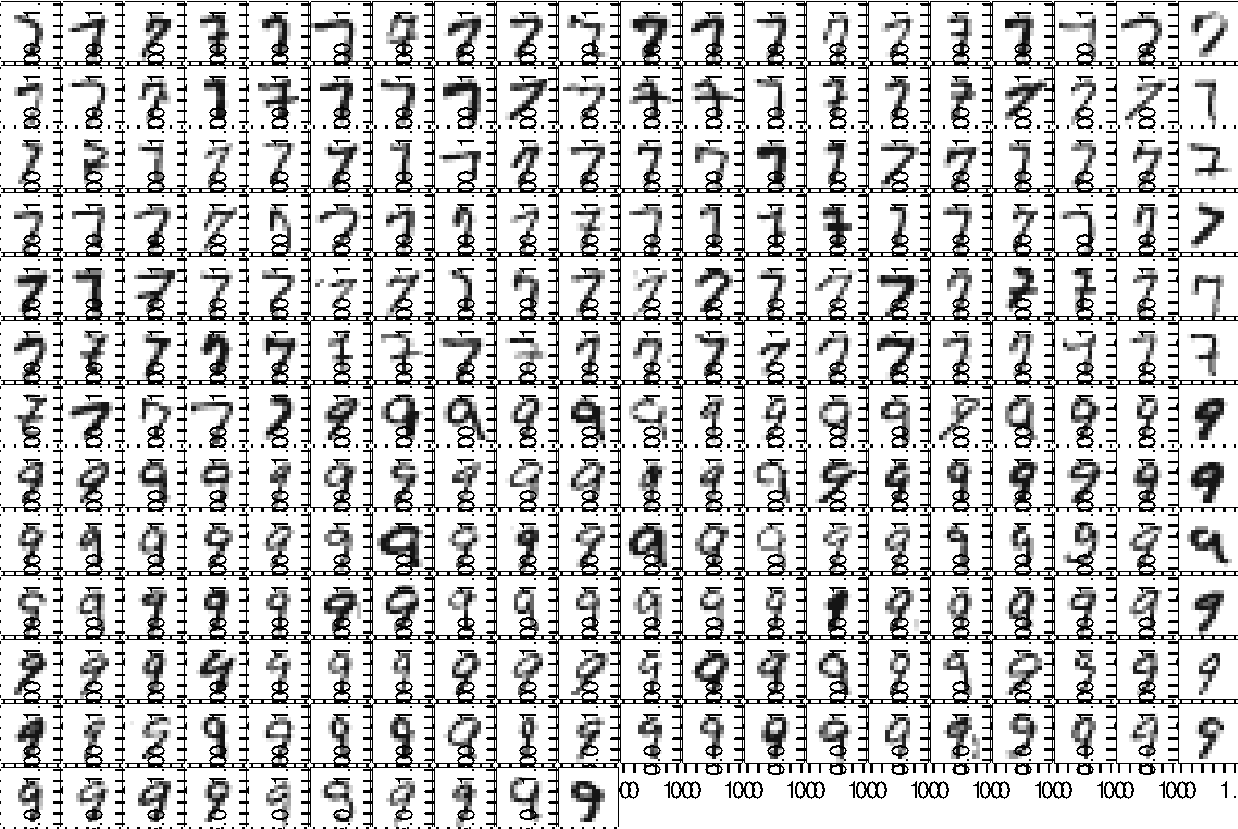
\includegraphics[width=1\linewidth]{ch-al/figures/data.pdf}
		\caption[MNIST data used in the simulations.]{MNIST data used in the 
		simulations. The digits 7 and 9 are relatively similar visually, making 
		the simulations more realistic as it is harder for the classificaiton 
		models to tell the difference.}
		\label{fig:al:simulations:data}
	\end{center}
\end{figure}

\subsection{Evaluation}
\label{sec:al:simulation:evaluation}
The performance of a learner at any given point in time (at any iteration 
\textit{i} of simulation number $k \in [1,25]$) is encapsulated in its error 
ratio $\epsilon$. That is, given the current labeled set, the \textbf{main 
classifier (Random Forest model)} is trained, and the entire dataset is 
predicted given the current classifier. The predictions are stored in an 
$n$-length vector $p$. 
We know the true labels ahead of time (thanks to the MNIST dataset), and they 
are stored in an $n$-length vector $y'$. The predictions are compared against 
the true labels and the error ratio of iteration $i$ is given by
$$\epsilon_i = \frac{1}{250} \bigg( \sum\limits_{z=1}^{250} 
\textbf{1}_{p_z \neq y'_z} \bigg)$$

\noindent where $\textbf{1}_{p_z \neq y'_z}$ is an indicator variable that is 1 
when $p_z \neq y'_z$ and 0 otherwise. These 50 error ratios then form one 
vector $\epsilon_s$, the result of trial 
$s$. To select the best active learning algorithm \textit{on average}, each 
algorithm's error ratios are averaged over 25 total trials. This helps offset 
the randomness of the initialization and pooling scheme. Then the final error 
ratio of an algorithm is given by
$$\epsilon = \frac{1}{25} \bigg( \sum\limits_{i=1}^{25} \epsilon_s \bigg)$$

The final framework for computing $\epsilon_s$, a single trial's vector of 
error ratios, is summarized as follows (This procedure is encapsulated by the 
simulation engine code in 
Appendix~\ref{sec:appendicies:al:simulations:simengine}):

\tablespacing
\begin{algorithm}[H]
	\caption{Computing $\epsilon_s$, a single trial's vector of error 
	ratios}\label{alg:al:simulation:evaluation}
	\begin{algorithmic}[1]
		\Procedure{}{$X$ is a $n\times d$ matrix of $d$ observations of all $n$ 
			variables, $y$ is an $n$-length vector of labels for each variable 
			in $X$ ($y_i$=N/A when $X_{i,}$ has no label). $y'$ is an 
			$n$-length vector of \textbf{true} labels for each variable in $X$. 
			$iter$ is the maximum number of queries allowed per trial}
		\State \textbf{loop from} $i=1$ \textbf{to} $iter$:
		\State \indent $idx \gets $ active\_learning\_method$(X,y,...)$
		\State \indent \textsc{Query} $X_{idx,}$
		\State \indent $tout \gets 
		\text{train}(X^{labeled},y^{labeled},\text{randomforest})$
		\State \indent $p \gets \text{predict}(tout,X)$
		\State \indent $res_i\gets \frac{\text{length}(\text{which}(p \neq y'))}
		{\text{length}(y')}$
		\State \textbf{return} $res$
		\EndProcedure
	\end{algorithmic}
\end{algorithm}
\bodyspacing

\subsection{Summary of methods}
\label{sec:al:simulation:methods}

What follows is a summary of the active learning methods used in the simulation 
with details such tuning parameter values.

\tablespacing
\begin{longtable}{p{0.15\linewidth} p{0.21\linewidth} p{0.18\linewidth} 
p{0.4\linewidth}}
	
	% First page heading
	\caption[Summary of simulation active learning methods.]{A summary of the  
	active learning methods tested in the simulation. *\textit{Note:} The 
	classification model is the main classification model that is used to fit 
	the error, not the classification model(s) used in the active learning 
	methods (those are parameters). 
	The classification model in the simulator is akin to the main 
	classification model in the VS.} 
	\label{tab:al:simulations}\\
	\toprule
	\textbf{AL method} & \textbf{Simulations} & 
	\textbf{Classification model*} & \textbf{Parameters} \\
	\midrule
	\endfirsthead
	
	% Future page heading
	\caption[]{(continued)}\\
	\toprule
	\textbf{AL method} & \textbf{Simulations} & \textbf{Main classification 
	model} & \textbf{Parameters} \\
	\midrule
	\endhead
	
	% Page footer
	\midrule
	\multicolumn{4}{r}{(Continued on next page)}\\
	\endfoot
	
	% Last page footer
	\bottomrule
	\endlastfoot
	
	Random \newline sampling \newline (CONTROL) & 
	25 trials, 50 iterations (queries allowed) each & 
	Random forest & 
	\textit{Classifier}: None \\
	
	\cmidrule[0.1pt](l{0.5em}r{0.5em}){1-4}	
	
	Uncertainty \newline sampling ~\ref{sec:al:methods:uncertainty} & 
	25 trials, 50 iterations (queries allowed) each & 
	Random forest & 
	\textit{Classifier}: Random forest \\

	\cmidrule[0.1pt](l{0.5em}r{0.5em}){1-4}
	
	Query by \newline committee ~\ref{sec:al:methods:qbc} & 
	25 trials, 50 iterations (queries allowed) each & 
	Random forest &	
	\textit{Committee}: RF, NB, SVM, PLS, \newline 
	\textit{Disagreement}: Vote entropy, \newline 
	\textit{C\_Pruning}: T, $\epsilon$: 0.5 \\ & \\
	
	& & Majority \newline committee \newline vote &	
	\textit{Committee}: RF, NB, SVM, PLS, \newline 
	\textit{Disagreement}: Vote entropy, \newline 
	\textit{C\_Pruning}: T, $\epsilon$: 0.5 \\ & \\
	
	& & Random forest &	
	\textit{Committee}: RF, NB, SVM, PLS, \newline 
	\textit{Disagreement}: Vote entropy, \newline 
	\textit{C\_Pruning}: F, $\epsilon$: N/A \\ & \\
	
	& & Majority \newline committee \newline vote &	
	\textit{Committee}: RF, NB, SVM, PLS, \newline 
	\textit{Disagreement}: Vote entropy, \newline 
	\textit{C\_Pruning}: F, $\epsilon$: N/A \\	
	
	\cmidrule[0.1pt](l{0.5em}r{0.5em}){1-4}	
	
	Query by \newline bagging ~\ref{sec:al:methods:bagging} & 
	25 trials, 50 iterations (queries allowed) each & 
	Random forest &
	\textit{Classifier}: Random forest, \newline \textit{Disagreement}: Vote 
	entropy, \newline \textit{num\_class}: 5, \textit{r}: 0.75 \\
		
	\cmidrule[0.1pt](l{0.5em}r{0.5em}){1-4}	
	
	Min-max \newline clustering ~\ref{sec:al:methods:clustering} & 
	25 trials, 50 iterations (queries allowed) each & 
	Random forest & 
	\textit{Classifier}: None, \newline \textit{Distance}: Euclidean \\
	
\end{longtable}
\bodyspacing

A summary of each classification model used in the stating committee for QBC 
implementation is as follows:

\tablespacing
\begin{itemize}
	\item \textbf{Random Forest:} A random forest is a collection of decision 
	trees which are grown from independent draws of the training set. A more 
	detailed description can be found in 
	Section~\ref{sec:visualizer:plotgeneration:tree}.
	\item \textbf{Naive Bayes:}
	\item \textbf{SVM:}
	\item \textbf{Partial Least Squares:}
\end{itemize}
\bodyspacing

The call to each active learning function is controlled by the AL engine code 
in Appendix~\ref{sec:appendicies:al:simulations:alengine}. By implementing the 
active learning call in this way, the main AL functions are hidden from the end 
user so that they cannot call the functions directly, which may lead to 
bypassing checks and/or improperly calling functions.



\subsection{Results}
\label{sec:al:simulation:results}

The full simulator which calls the aforementioned engines, runs the 25 
simulations, and plots the results may be found in 
Appendix~\ref{sec:appendicies:al:simulations:results}.
The results are summarized in the line plot below.

(Discuss how QBC actually spikes up when the pruning occurs, contrary to 
intuition - perhaps there is room for a future extension there. Note that the 
simulations are in no way completely comprehensive/exhaustive, and there is 
further work 
to be done ... For example, trying other classification models within the 
active learning algorithms - who knows, maybe that would've been better! Or 
trying different QBC committees, different tuning parameters i.e. pruning 
factor is 0.75 instead of 0.5, or you prune later/earlier)

%streaming method (given 15random points, label them, then use AL criteria to 
%pick the next point to query)
%More feasible for the VS since we would have to know what each plot looks 
%like, and there's just too many plots (d choose 2?) to be computationally fast
%
% versus
%
%overall method (look at all points, label them, then use AL criteria to pick 
%the next point to query)
\chapter{Graph comparison \label{ch:gc}}

Introduction/how it relates to the VS (rehash end of chapter 2)

\section{Graph summarization}
\label{sec:gc:litreview}

There are two ways of thinking about graph comparison. Let 
$\hat{G^1}=(V^1,E^1)$ and $\hat{G^2}=(V^2,E^2)$ each be some labeled graph. 

\tablespacing
\begin{enumerate}
	\item \textbf{Graph summarization:} Compute some vector 
	$v^1$ on $\hat{G^1}$ that ``summarizes'' various properties that
	it has. Similarly, compute $v^2$ on $\hat{G^2}$ to capture 
	the same properties that $v^1$ does. Finally, compute 
	$f(v^1,v^2)$ where $f$ is some distance 
	function (e.g. Euclidean distance). A high value indicates strong 
	dissimilarity while a low value indicates similarity. 
	
	\item \textbf{Graph distance:} Create a valid distance function $f$ on the 
	graphs $\hat{G^1}, \hat{G^2}$ directly rather than a vector of metrics 
	($v^1,v^2$). 
	Compute $f(\hat{G^1},\hat{G^2})$. Again, a high value indicates strong 
	dissimilarity while a low value indicates similarity. The \textit{random 
	walk kernel} is one such example of a graph distance 
	metric~\cite{vishwanathan2010}.
\end{enumerate}
\bodyspacing

We specifically focus on the graph summarization comparison because it 
fulfills both desired criteria for the visualization system; an understanding 
of each summarization method allows the user to gain intuition on the qualities 
of the graph, and the difference between two graph summarization methods can be 
quantified easily. To be more specific, we seek to better understand the 
qualities of existing graph summarization methods and their associated 
advantages and disadvantages. 
Understanding these metrics is important due to the complex nature of graphs.
It is natural to ask why we cannot just plot the graphs instead (which are 
typically in the form of either an adjacency matrix of list of edges) and 
examine the result for visual patterns in order to understand the qualities 
of the graph. This is unfeasible for several reasons (see 
Figure~\ref{fig:gc:arr_density}). 

\tablespacing
\begin{itemize}
	\item \textbf{Arrangement:} Different arrangements of nodes on the visual 
	plane may have a profound effect on the interpretability of the graph; from 
	the start, it is unclear what the best arrangement might be, and it is 
	unfeasible for an analyst to try all possible arrangements 
	especially as the number of variables increase.
	
	\item \textbf{Density:} The more nodes there are, the more edges there may 
	be, and the more dense a graph may become, making it incredibly difficult 
	to interpret. Furthermore, it makes it more difficult to find anomalies 
	among the variable's relationships (represented by edges). A non-existent 
	edge in a dense graph is just as important as an existent edge in a sparse 
	graph because each indicates a relationship which isn't quite like all the 
	others.
\end{itemize}
\bodyspacing

\begin{figure}[htb]
	\begin{center}
		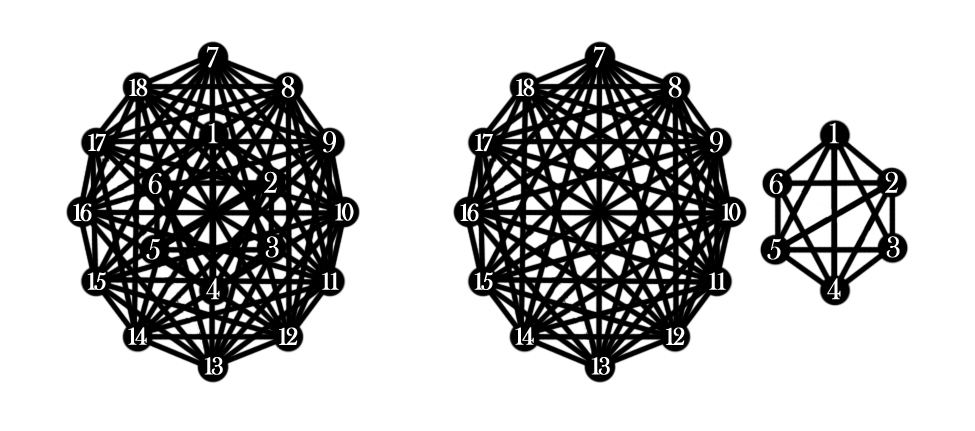
\includegraphics[width=1\linewidth]{ch-gc/figures/arr_density}
		\caption[Difficulties with graph visualization.]{
		Suppose we have a graph $G=(V,E)$ with clusters $C^1,C^2$ and $|V|=18$. 
		Let $C^1$ be composed of nodes $(V_1,...,V_6)$, and $C^2$ be composed 
		of nodes $(V_7,...,V_{18})$. 
		\textit{Left:} $C^1$, the smaller cluster, has been placed inside 
		$C^2$, the larger cluster. It is difficult to discern any meaningful 
		patterns; each node appears to be connected to every other node as the 
		density of the cluster $C^2$ makes it almost impossible to see that of 
		$C^1$.
		\textit{Right:} The nodes have been rearranged in a manner that clearly 
		distinguishes between $C^1$ and $C^2$. At a glance, it is evident that 
		$C^1$ is missing $E_{3,6}$. It is difficult to tell, however, that 
		$C^2$ is even missing an edge $(E_{13,17})$ in the first place!
		$C^1$ is more sparse, which makes it easier to visually perceive 
		anomalies in the graph.}
		\label{fig:gc:arr_density}
	\end{center}
\end{figure}

Graph summarization acts as a proxy for visually exploring the graph 
itself. Each metric, which is associated with a different characteristic of the 
graph, can be parsed and later combined to 
``reconstruct'' or better understand the qualities of each graph, subsequently 
allowing the user to better understand \textit{exactly where} the visual and 
numeric graphs differ (should the final graph comparison metric suggest that 
the two graphs are highly different). Graph distance functions skip that 
critical step by going through 
the graphs directly.

To put it in another way, graph summarization has the \textit{exact opposite 
problem} that is present in data analytics as it is practiced today (discussed 
in Chapter~\ref{ch:intro}, this is the motivation behind the VS and this 
thesis). 
The visualization system allows the user to use the visual qualities of pairwise
scatter plots to better understand numerical qualities of the data, but graph 
summarization allows the user to use numerical qualities to better understand 
the visual qualities of a graph. 

With an understanding of the properties of various graph summarization methods, 
the graph summarization difference metric may be more informative. In the VS, 
the graph summarization difference computes a list of graph summarization 
metrics $(m^\text{num},m^\text{vis})$ for each graph in order to provide a 
single vector $d$ that quantifies the difference between them with 
some difference function (e.g. Euclidean distance, L2, etc.). 
As such, a natural byproduct of the computation is 
$(m^\text{num},m^\text{vis})$, which (armed 
with an understanding of the values) provides insight on the qualities of the 
visual graph and numerical graph \textit{on an individual level} and where 
exactly their differences and similarities lie.
\section{Overview of graph summarization methods}
\label{sec:gc:methods}

\subsection{Centrality}

\subsection{Community}

\subsection{Distance matrix}

\subsection{Assortativity}

\subsection{Edge density}

\subsection{Edge connectivity}
\section{Examples}
\label{sec:gc:examples}

Table summarization of method outputs when applied to various examples we've 
thought of previously

\chapter{Results\label{ch:usage}}

Use the WHOLE visualizer system (with aforementioned inputs from ch 3 and 4) on the data

Compare results to numericala results

\section{Application of the visualization system}
\label{sec:usage:newanalysis}

Now the issue is that there are many correlation graphs which may be 
computed with different correlation coefficients; given the large dataset, it 
is unclear which metric might be the best one. This is where the visualization 
system comes in and ties everything together. By learning the user's interests 
and automatically labeling correlated vs uncorrelated pairs of variables, the 
VS outputs a visual correlation graph that may be used as a ``sanity check'' 
against the various numerical correlation graphs and provide a guide for 
selecting the most intuitive numerical correlation graph.

Let $X$ be a $n\times d$ data matrix where there are $n$ observations of $d$ 
variables. The final procedure is as follows:

\tablespacing
\begin{enumerate}
	\item Create four different numerical correlation graphs 
	$G^i=(V,E)$ where $|V| = d$ for all $i\in \{1,...,4\}$ with 
	threshold $t = 0.15$, one for each correlation coefficient described in 
	Section~\ref{sec:intro:correlation} (Pearson's, Spearman's, Kendall's, and 
	distance correlation).
	
	\item Run the VS on the same dataset. Stage 1 of the system utilizes the 
	active learning algorithm selected in Chapter~\ref{ch:al} to learn what is 
	``correlated'' and ``not correlated.'' Stage 2 of the system then iterates 
	through all possible unlabeled plot pairs and returns a visual graph 
	$G=(V,E)$ where 

\begin{algorithm}
	For $i,j\in \{1,...,d\}$, $E_{i,j}$ exists if the plot of $j$ against $i$ 
	is ``correlated''
\end{algorithm}

	As a reminder, correlation is used loosely to refer to a visual 
	interpretation of the mathematical term.

	\item Utilize the graph comparison methodology explained in 
	Chapter~\ref{ch:gc} to find the difference of each pair 
	$(G,G^i)$ for all $i \in \{1,...,4\}$. Select numerical graph $G^*$ such 
	that $\text{diff}(G,G^*) \leq \text{diff}(G,G^i)$ for all $i\in 
	\{1,...,4\}$. The numerical correlation graph $G^*$ is then the graph which 
	best matches the visual interpretation of the relationships among the 
	dataset's variables.
	
	\item Using the stock selection procedure in 
	Section~\ref{sec:usage:stockselection}, create a portfolio $P^i$ from each 
	graph $G^i$ (including portfolio $P^*$ from the graph selected as $G^*$). 
	
	\item Observe the performance of each portfolio until 2014.
\end{enumerate}
\bodyspacing

Normally, it would be standard to simply use the selection procedure with $G^*$ 
as an input to determine the desired ``buy and hold'' portfolio, record the 
yearly returns, and then be done. However, because the purpose of this chapter 
is to demonstrate the usage and viability of the VS in aiding with the selectio 
of an appropriate numerical procedure (given a dataset and some desired 
purpose), it is necessary to compare the results of all options among one 
another. 
It is natural to expect that the portfolio $P^*$ will perform the best 
as that is the purpose of the visualization system, after all. 
By comparing the results of $P^*$ against the other numerical options, we may 
determine just how well the system captured the user's intuition regarding 
independence (which is not as straightforward as a simple metric).
It should also be noted that, while a rebalancing method performs better in 
practice~\cite{liuh2016}, the ``buy and hold'' is better-suited for observing 
the portfolio performances over time, providing a more concrete basis of 
comparison for the selected correlation coefficient. The final code for the 
application procedure may be found in 
Appendix~\ref{sec:appendicies:usage:newanalysis}. 
\section{Results}
\label{sec:usage:results}

The specific queries given by the VS and the corresponding oracle labels 
(the oracle, in this case, is the author of this work) may be seen in 
Figures~\ref{fig:usage:interesting} and \ref{fig:usage:notinteresting}. Recall 
that the active learner in stage 1 was given a budget of 15 queries. The 
queried plots are not labeled during stage 1 in order to prevent potential bias 
from clouding the oracle's responses. After stage 2, the user may plot and view 
the corresponding variable names should he/she wish to do so.

\newpage 
\begin{figure}[htb]
	\begin{center}
		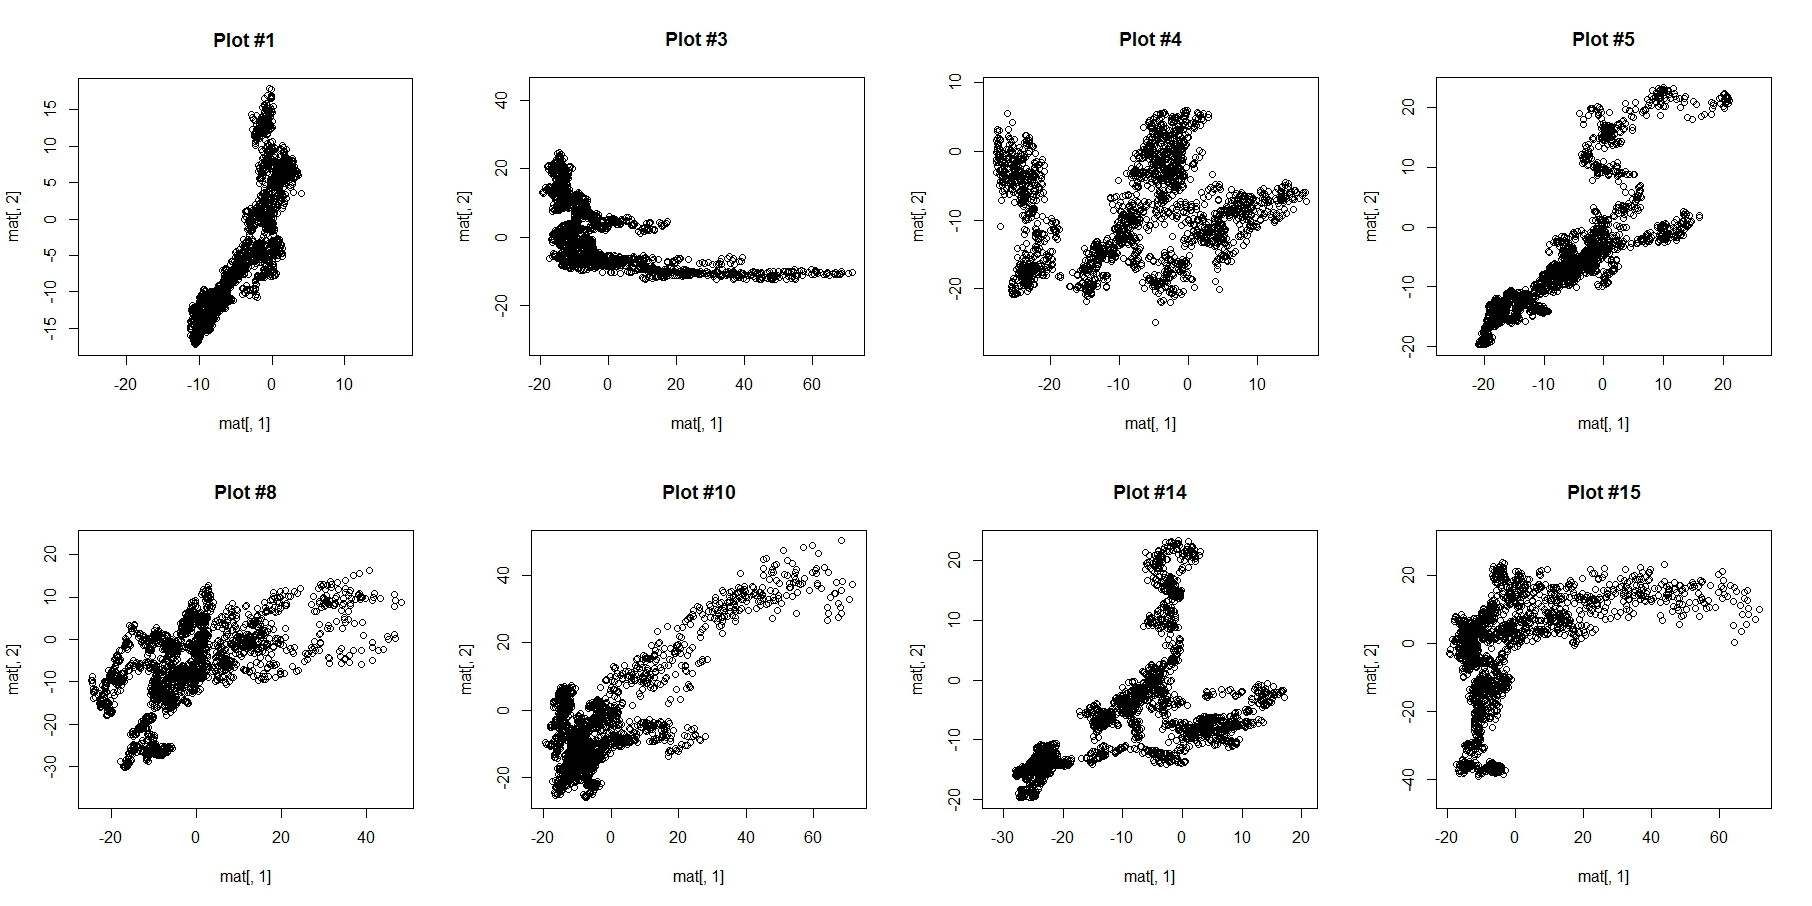
\includegraphics[width=1\linewidth]{ch-usage/figures/y_all}
		\caption[VS queries which were labeled ``visually correlated''.]{VS 
		queries which were labeled ``visually correlated''.}
		\label{fig:usage:interesting}
	\end{center}
\end{figure}

\begin{figure}[H]
	\begin{center}
		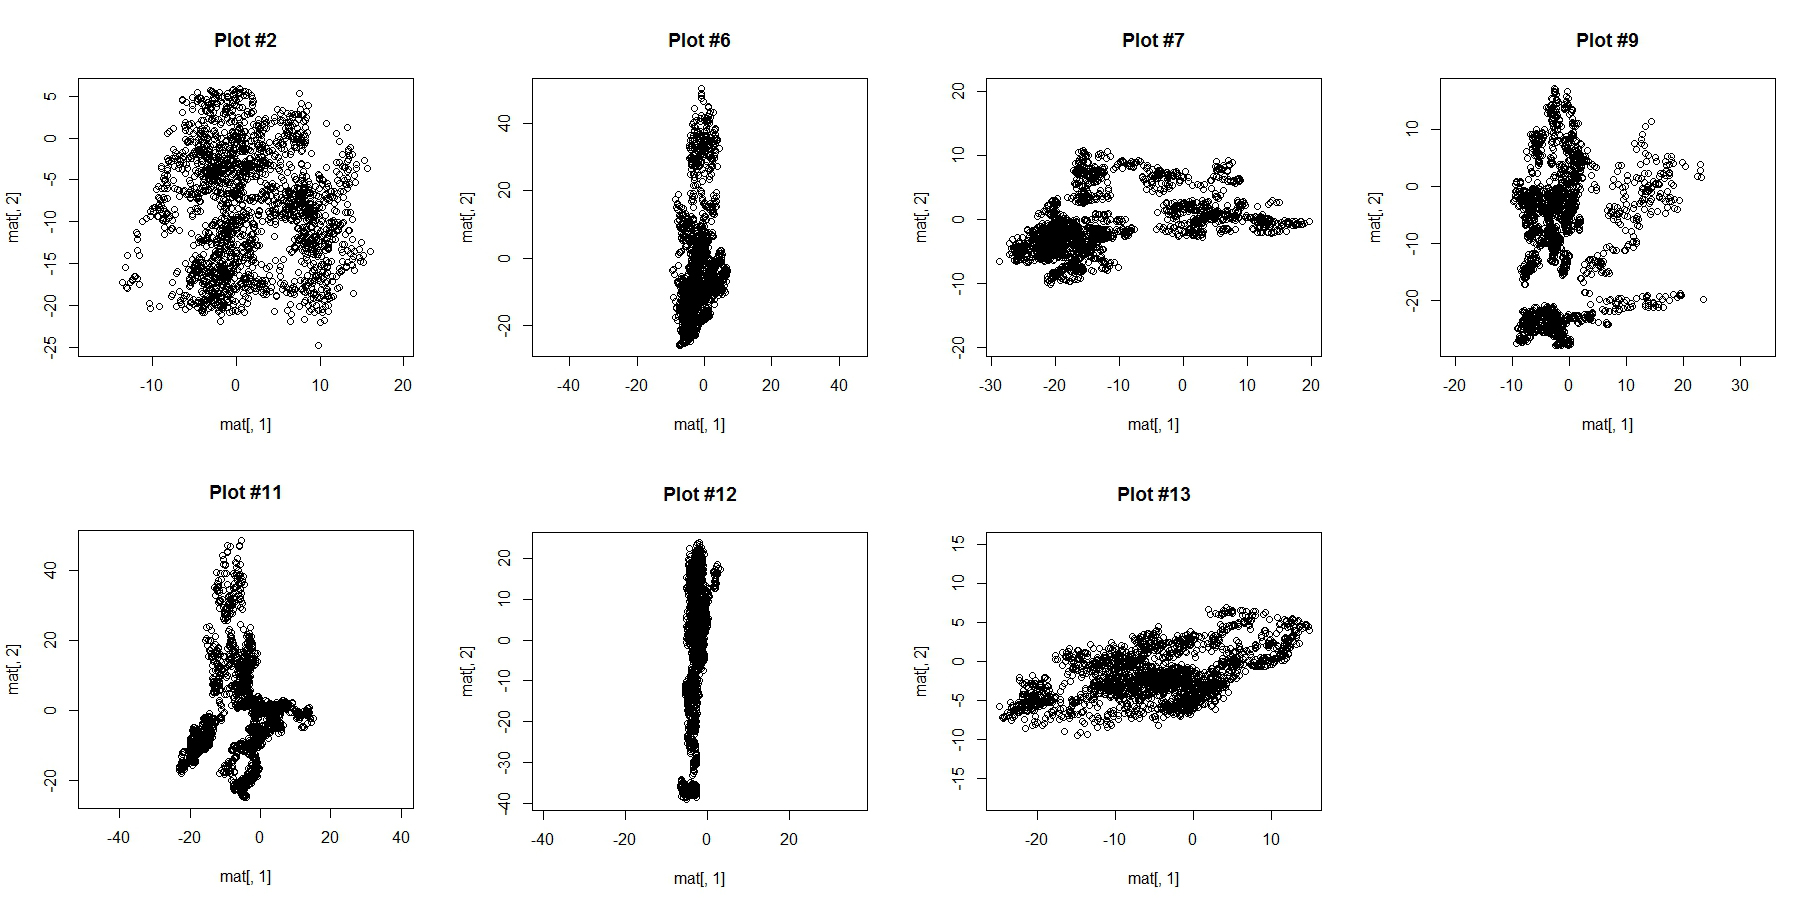
\includegraphics[width=1\linewidth]{ch-usage/figures/n_all}
		\caption[VS queries which were labeled ``not visually correlated''.]{VS 
		queries which were labeled ``not visually correlated''.}
		\label{fig:usage:notinteresting}
	\end{center}
\end{figure}

It is also interesting to examine the heat maps (which are normalized) that 
correspond to the 15 queries; these heat maps may be found 
in Figure~\ref{fig:usage:heatmaps}, which also contains a list of associated 
criterion. A quick glance at the heat maps reveal that 
the middle criteria are all zero. It actually turns out that these criteria 
are associated with various Pearson correlation tests. 
The zero-value heat map entries indicate that the associated $p$-values are all 
extremely low (the correlation is significantly different from zero). In 
particular, this indicates that the criterion 9, 10, 11, 12, 13, and 14 are 
all significant. Consider the actual variable pairs associated with these 
criteria. The first row corresponds to the first queried plot which received a 
label of ``not visually interesting'' (It is the top left plot depicted in 
Figure~\ref{fig:usage:notinteresting}). Specifically, the pair has a Pearson 
correlation coefficient of -0.069 and $p$-value of 0.001728. The Pearson 
correlation coefficient is actually rather close to 0 
(uncorrelated) despite the $p$-value suggesting otherwise. When looking at the 
metric numerically as the heat map does, the natural response would be to draw 
an edge as in the $p$-value heuristic given in 
Section~\ref{sec:intro:correlation}. 
However, visually examining the pair's scatter plot (and even just looking at 
the correlation coefficient without the $p$-value) makes it clear that the pair 
is uncorrelated. How did this happen? Because there are 2050 observations of 
each stock, the variance, and subsequently the $p$-value, is low. 
If the correlation graph was constructed solely based on 
the Pearson correlation coefficient $p$-value without consideration of other 
factors, the result would have been less than ideal. This is another scenario 
that demonstrates the usefulness of the VS.

\begin{figure}[H]
	\begin{center}
		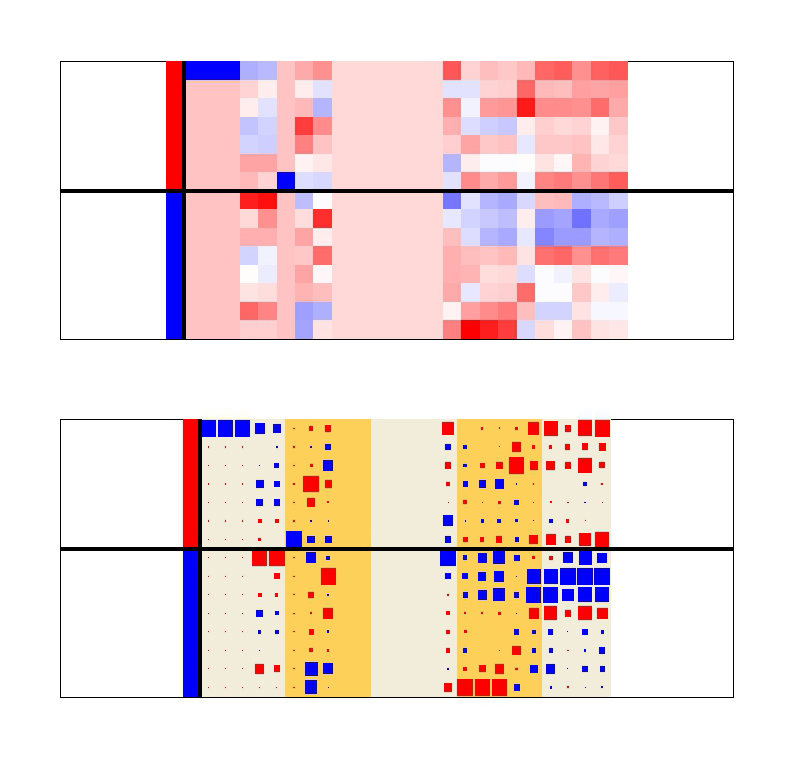
\includegraphics[width=0.8\linewidth]
		{ch-usage/figures/heatmaps}
		\caption[Normalized heat maps of VS queries and user-specified labels.] 
		{\textit{Top:} Standard heat map of the queries and given labels 
		(normalized). 
		\textit{Bottom:} Revised heat map (the association navigator) as 
		proposed by Buja \textit{et al.}~\cite{buja2016} (also normalized). 
		Each row corresponds to a pairwise scatter plot queried by the VS in 
		stage 1. Each scatter plot is ordered by 
		the oracle's responses; red indicates ``not visually correlated'' 
		and blue indicates ``visually correlated'' (as dictated by the 
		oracle). Each column 
		corresponds to a different criterion of the associated pairwise 
		scatterplot (see Section~\ref{sec:visualizer:scatterplot}). Ordered 
		criterion list (left to right, up to down): 
		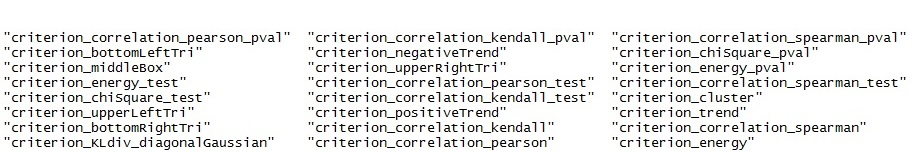
\includegraphics[width=1\linewidth]{ch-usage/figures/criterionlist}}
		\label{fig:usage:heatmaps}
	\end{center}
\end{figure}

Figure~\ref{fig:usage:hist} is a predicted probability histogram. The 
probability of being ``visually interesting'' or not is computed for 100 random 
pairwise scatter plots. Each probability is computed using the final 
classifier output from stages 1 and 2 of the VS. Most of the pairs fall within 
two bins (low and high probability). This can be observed as the two upper and 
lower hills in the histogram, indicating that the final classifier 
determined by the VS is quite confident in its labeling of most of the scatter 
plots.

\begin{figure}[htb]
	\begin{center}
		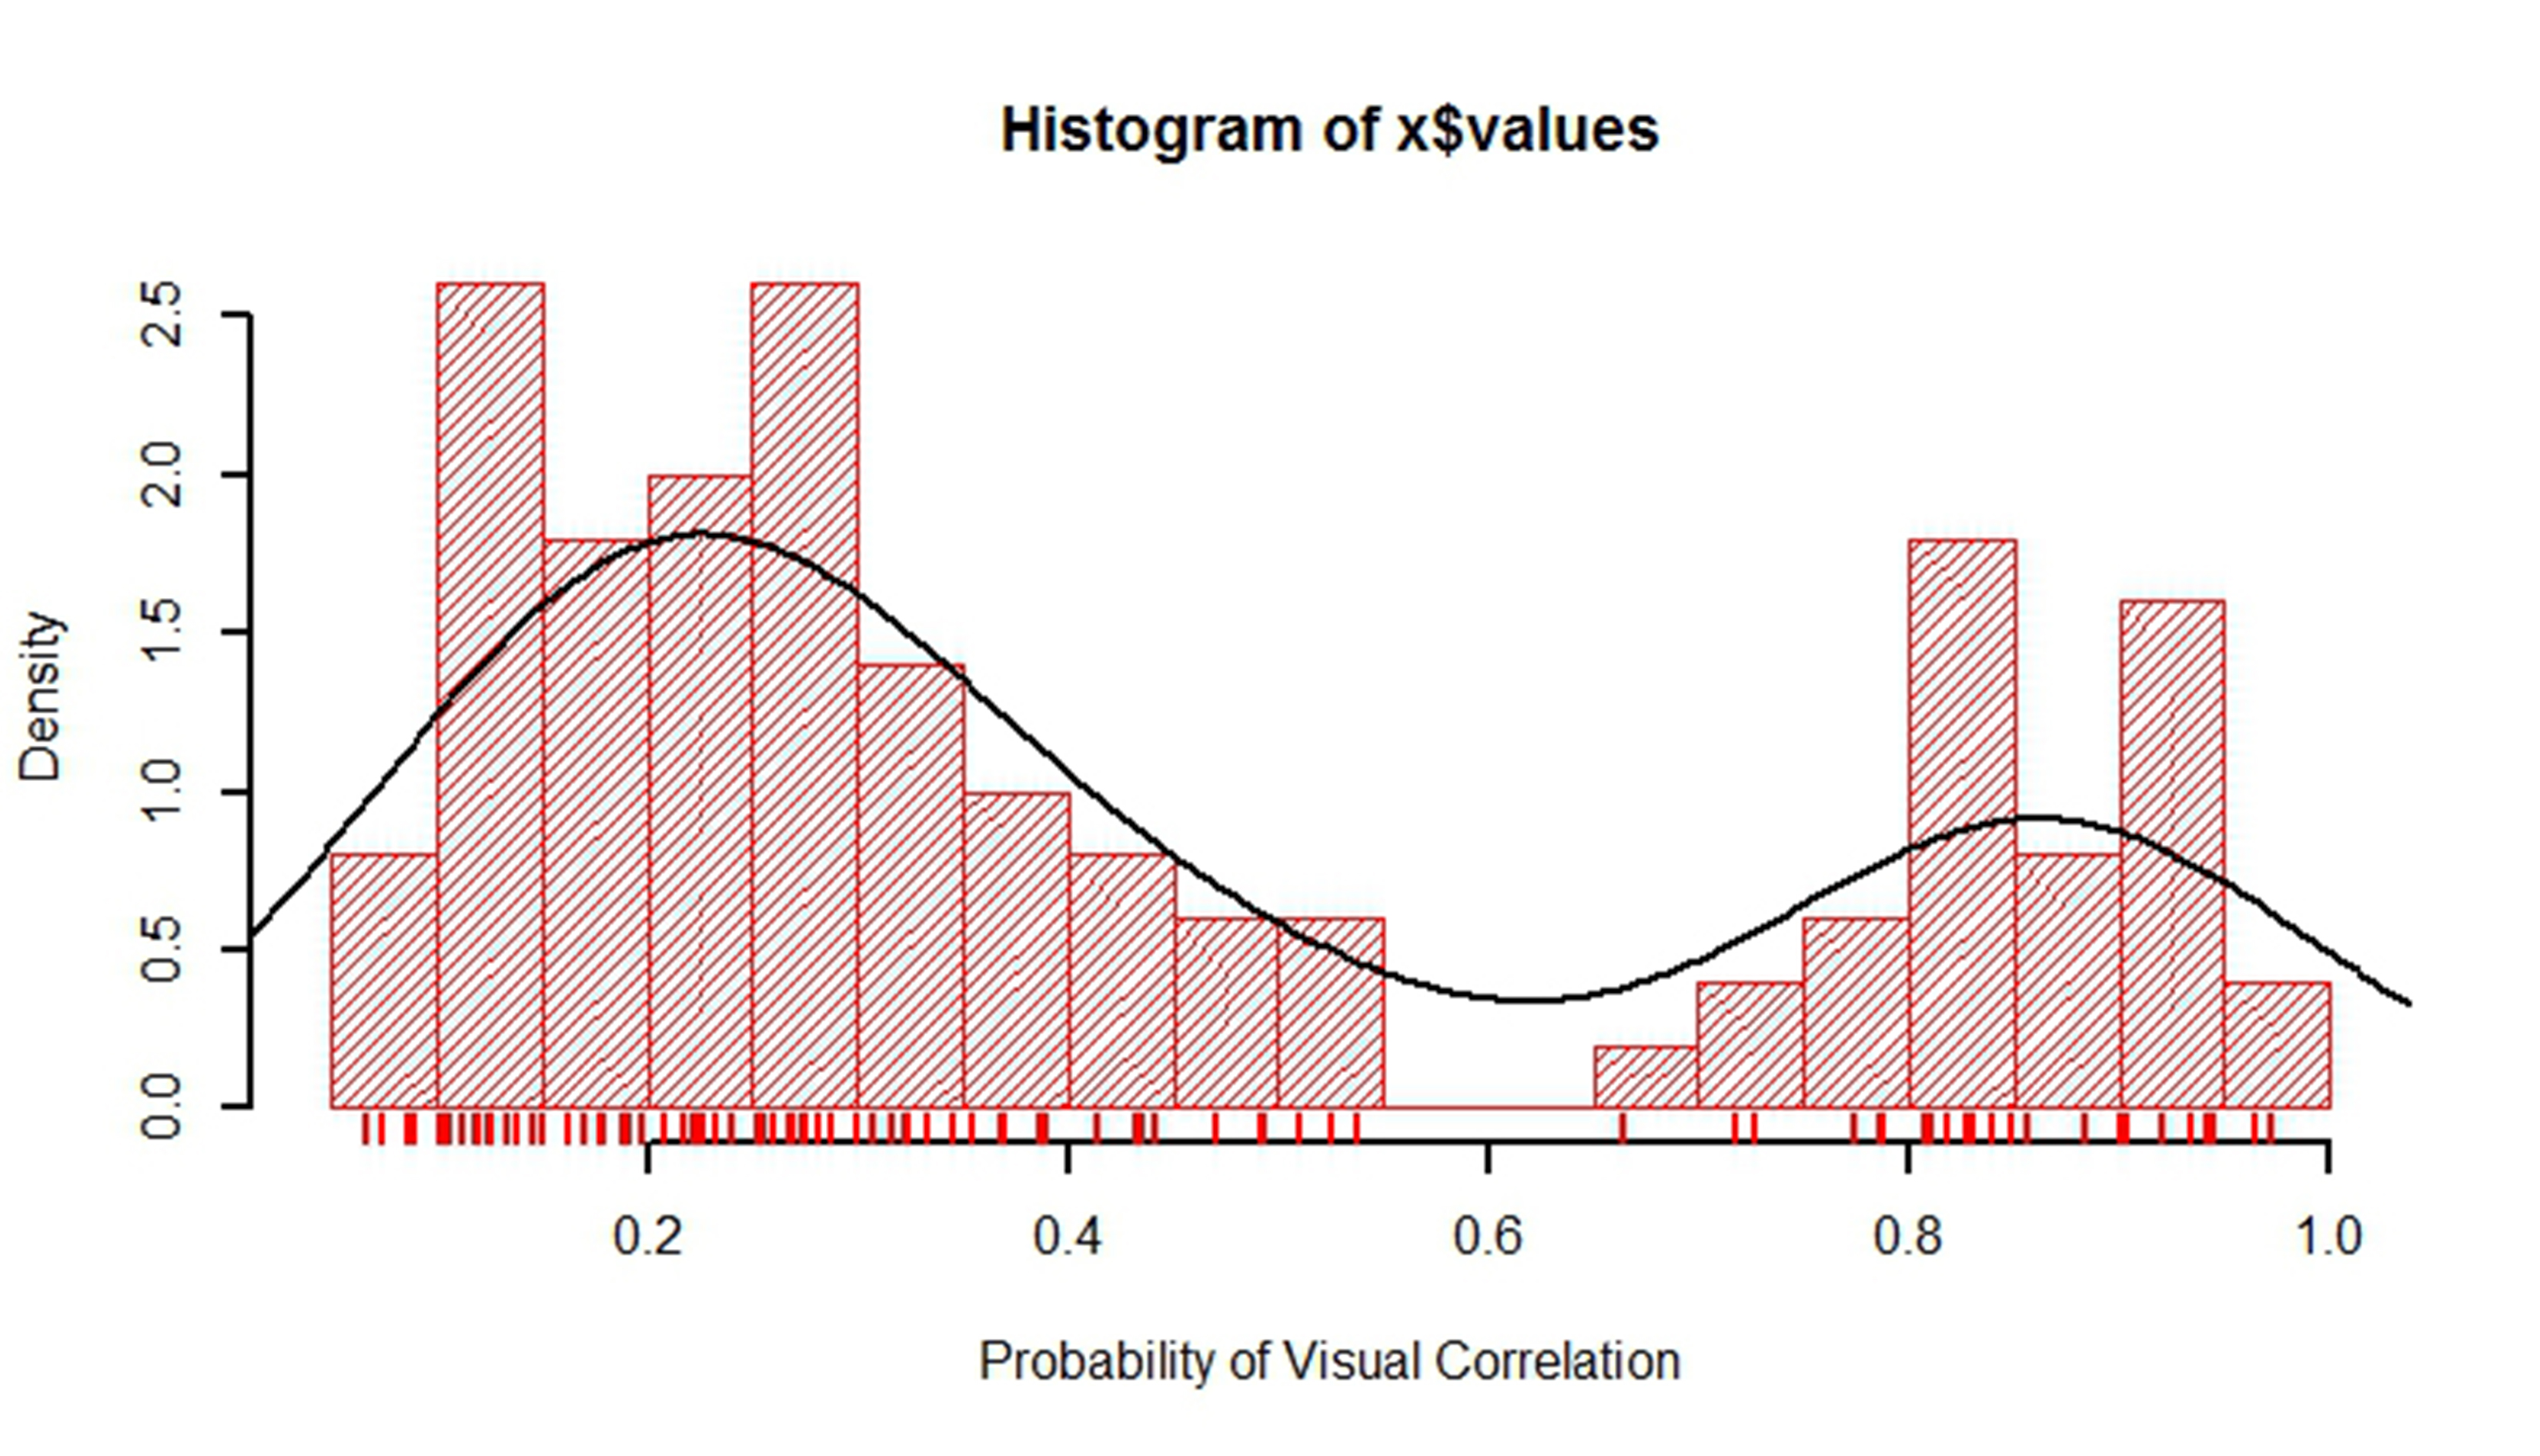
\includegraphics[width=1\linewidth]
		{ch-usage/figures/predicted_probability_histogram}
		\caption[Histogram of predicted probabilities.]{The histogram shows the 
		predicted probabilities for 100 pairwise scatter plots. The 
		probability corresponds to the probability of a plot being 
		``visually correlated'' or ``not visually correlated''.}
		\label{fig:usage:hist}
	\end{center}
\end{figure}

\begin{figure}[htb]
	\begin{center}
		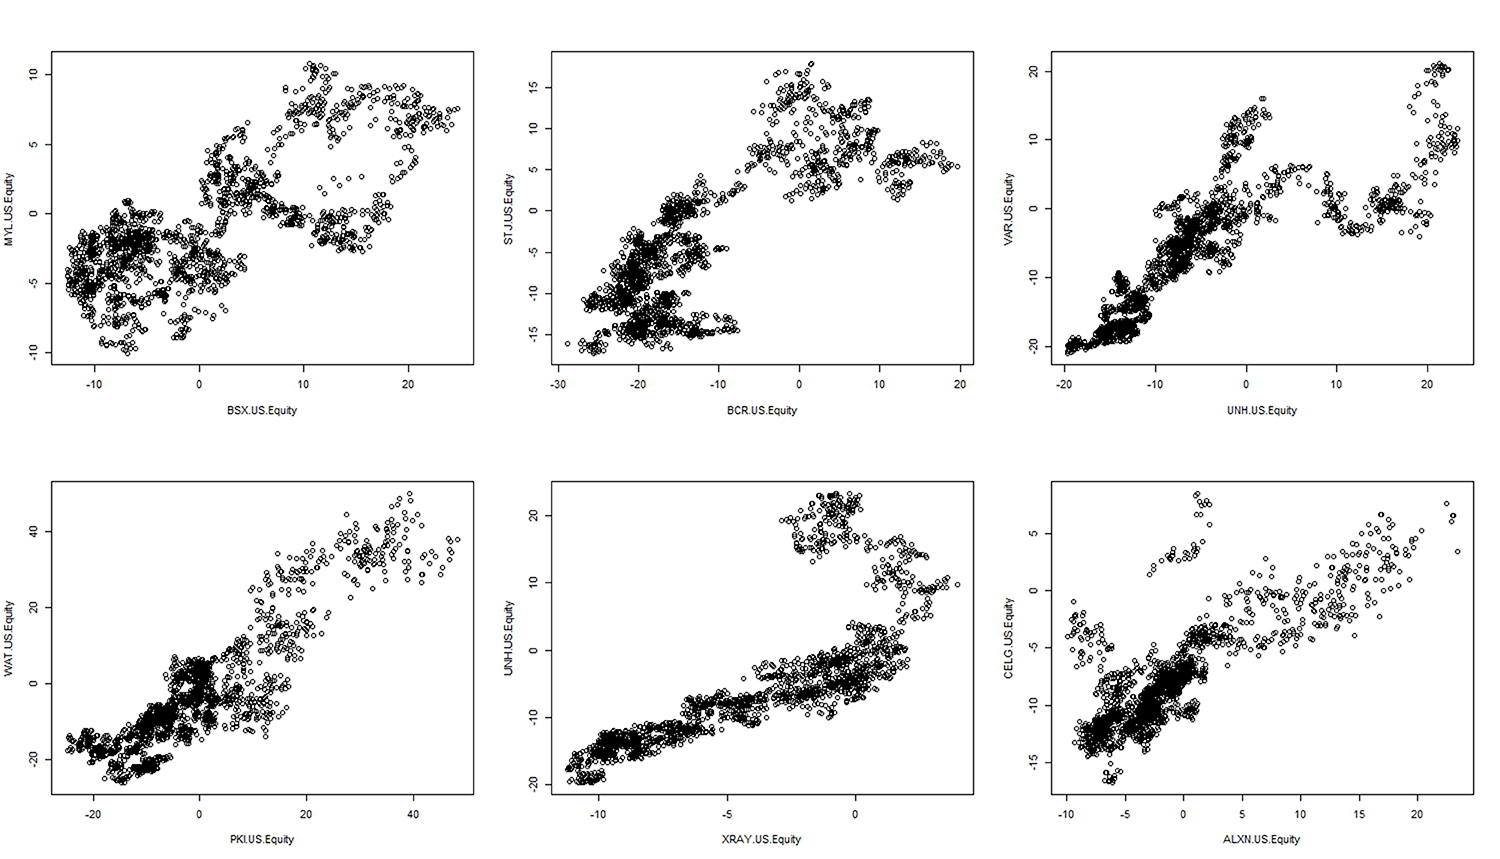
\includegraphics[width=1\linewidth]
		{ch-usage/figures/topinterestingplots}
		\caption[Top six most ``visually correlated'' pairwise scatter plots	
		selected by the VS.]{Top six most ``visually correlated'' pairwise 
		scatter plots selected by the VS.}
		\label{fig:usage:interestingplots}
	\end{center}
\end{figure}

\newpage
Figure~\ref{fig:usage:interestingplots} contains the most interesting plots 
selected by the VS in the automatic plot generation output of the VS. 
Interestingly, none of the variables (stocks) which are involved in these plots 
ever show up twice. Most of these plots exhibit a strong positive trend.
The final resulting visual correlation graph is shown in 
Figure~\ref{fig:usage:visg}. Interestingly, only stock 39 (which corresponds to 
ticker TMO) is in its own cluster; in fact, its degree is zero! This indicates 
that TMO is one of the best stocks to select because it is ``visually not 
correlated'' and, by proxy, independent of all other stocks.

\begin{figure}[H]
	\begin{center}
		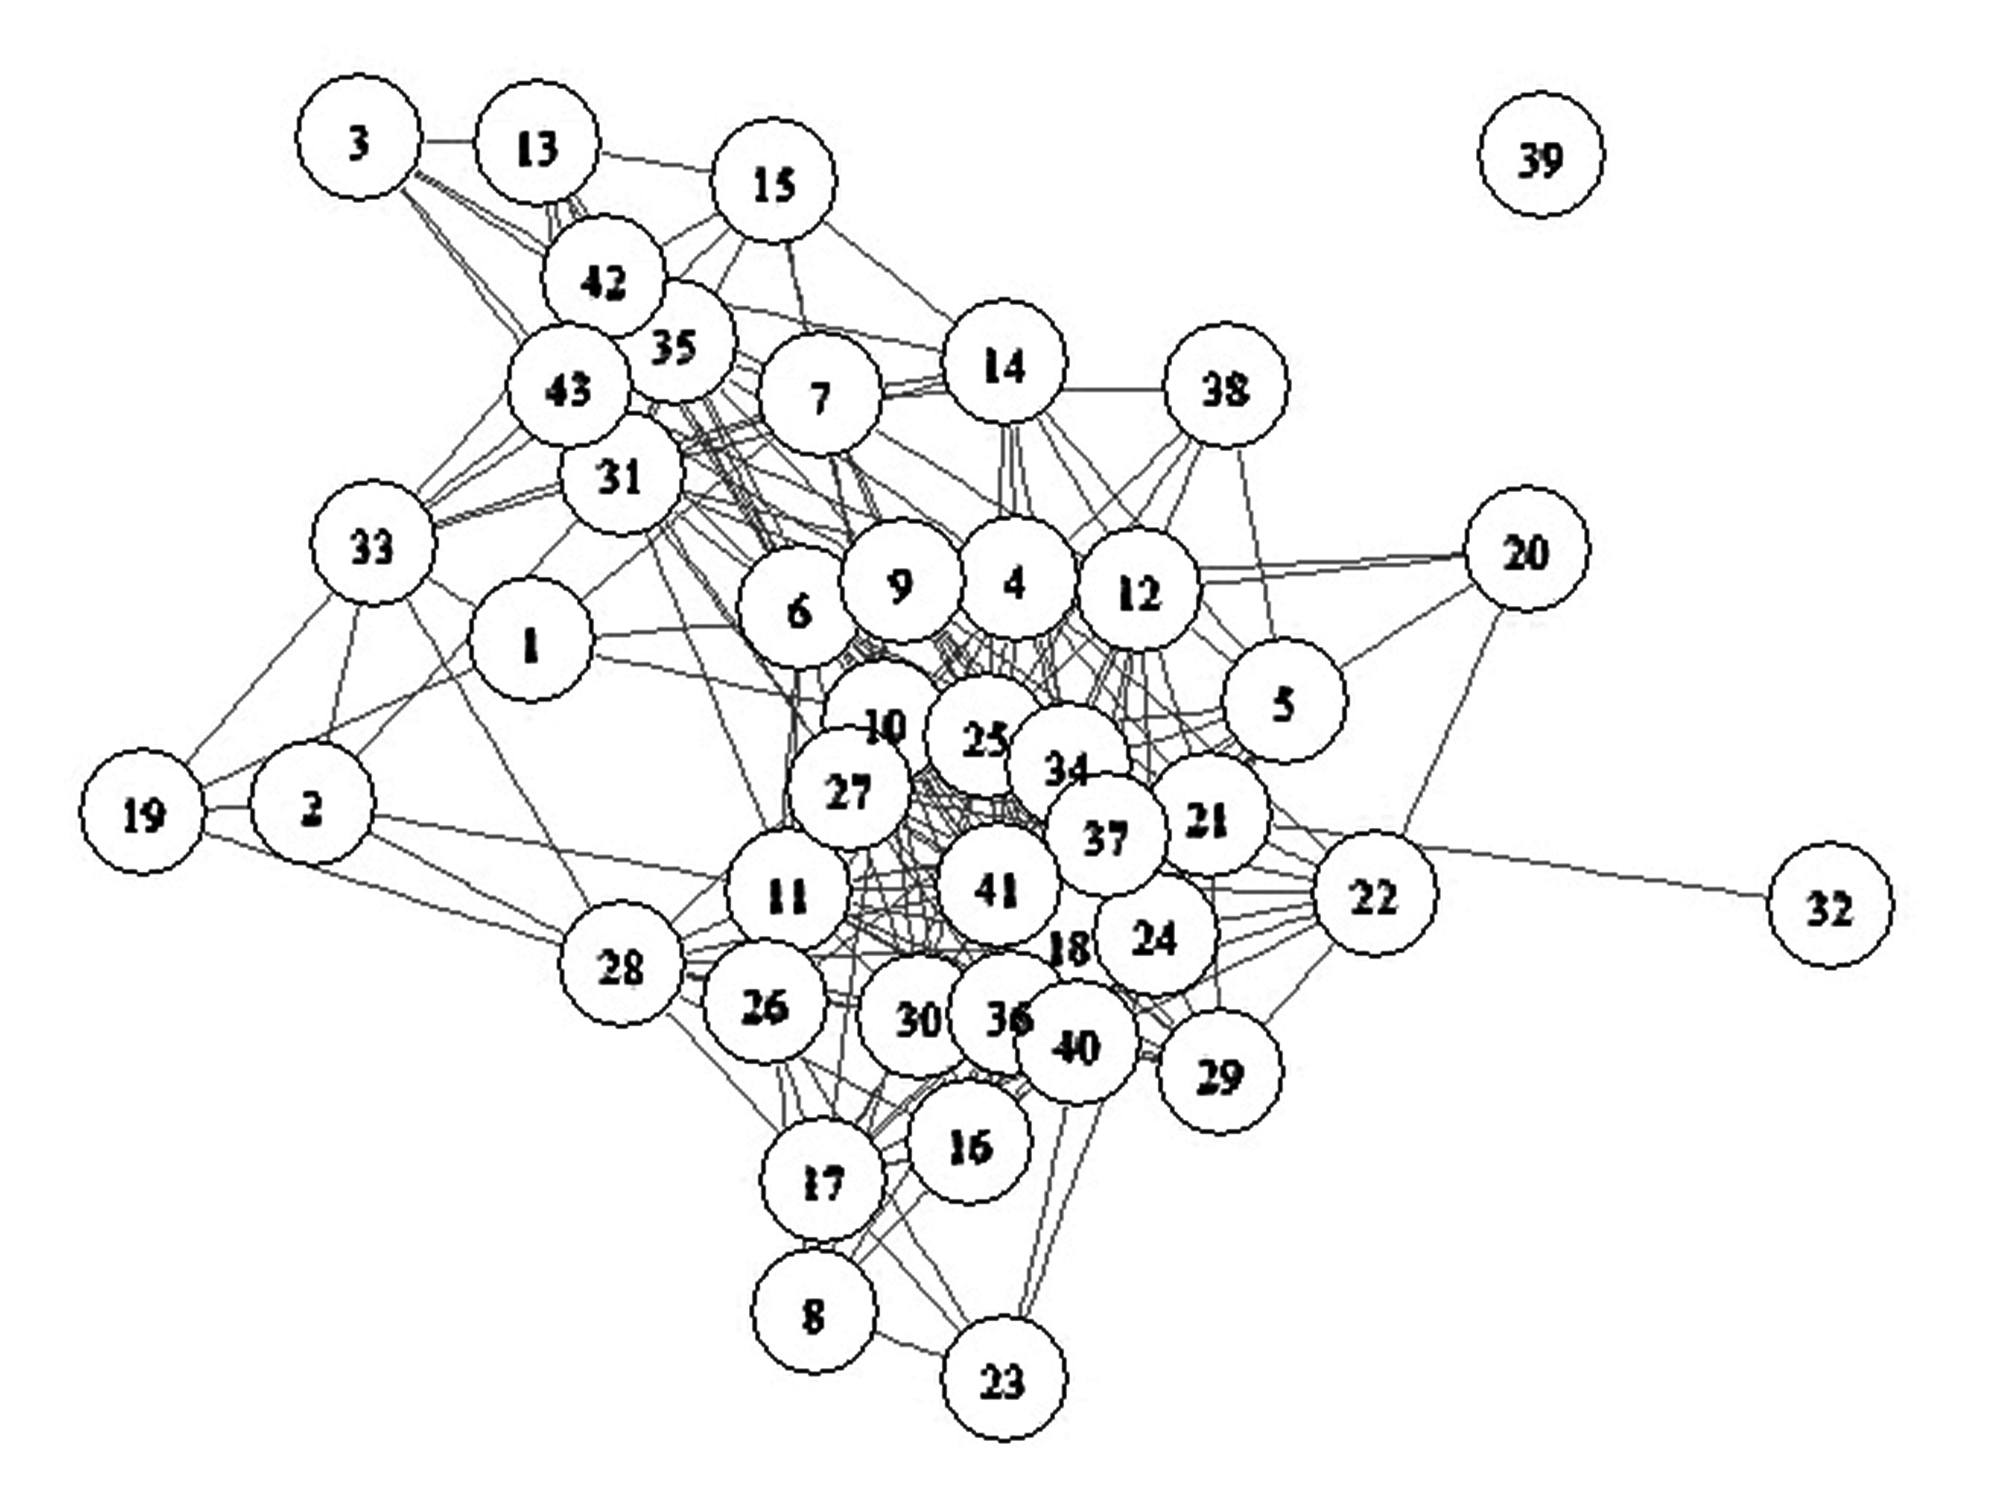
\includegraphics[width=0.75\linewidth]
		{ch-usage/figures/visgraph}
		\caption[Visual correlation graph output from the visualization 
		system.]{Visual correlation
		graph output from the visualization system.}
		\label{fig:usage:visg}
	\end{center}
\end{figure}

The graph comparison procedure determined that the \textbf{distance correlation 
graph} is closest to the visual correlation graph. 
The computed graph differences may be found in Table~\ref{tab:usage:graphdiff}.
The resulting portfolios selected by the procedure in 
Section~\ref{sec:usage:stockselection} for each numerical correlation graph are 
summarized in Table~\ref{tab:usage:returns}. Only the Pearson's correlation 
graph and distance correlation graph include TMO, the most ``visually not 
correlated'' stock, in their portfolios. 

Finally, the the ``buy and hold'' performance (yearly returns) and cumulative 
sum of returns are plotted for the S\&P 500 (the control) and
all portfolios $P^i$ for $i \in \{1,...,4\}$ may be found in 
Figure~\ref{fig:usage:returns}. Each portfolio $P^i$ was created 
from its corresponding numerical correlation graph $\hat{G}^{i,\text{num}}$ and 
includes $P^*$, which is created from $\hat{G}^* = \hat{G}^{4,\text{num}}$ 
(which corresponds to the distance correlation graph). The associated 
data may be found in Table~\ref{tab:usage:returns}. Note 
that the returns for 2006 and 2014 are low because the data begins 
on 3/14/2006 and ends on 5/13/2004; as such, the returns for 2006 and 2014 do 
not reflect a full year's worth of data. Our focus is mostly diverted to the 
full years in between and especially the portfolio performance during the 
financial crisis. 

The portfolio $P^*$, constructed from the numerical distance correlation graph 
$\hat{G}^*$ that is most similar to the visual correlation graph $\hat{G}$, 
performs the strongest by far. $P^*$ consistently posts the highest returns 
year after year. Though it doesn't seem to strongly outperform on a yearly 
basis, the differences really add up as can be seen in cumulative sum of yearly 
returns. Further 
consider the financial crisis; $P^*$ has the least negative returns of 2008. 
This indicates that the visual graph is capturing the independence and 
dependence among various stocks properly, which translates into the selection 
of $\hat{G}^*$ and, subsequently, $P^*$, a portfolio that is well balanced and 
captures the spirit of the ``buy and hold'' model described in 
Section~\ref{sec:intro:finance}.
Although the Pearson's correlation portfolio also included TMO, it 
performed rather average; it seems that linearity was not enough to 
capture the relationships among the other stocks.
As noted earlier in Section~\ref{sec:usage:stockselection}, the proposed stock 
selection strategy is simple, but every selected portfolio has outperformed the 
S\&P 500, suggesting that an even more sophisticated selection procedure would 
yield even more fruitful returns.

\subsubsection{Extensions}

It should also be noted that, while a rebalancing method performs better in 
practice~\cite{liuh2016}, the ``buy and hold'' strategy is better-suited for 
observing portfolio performances over time with less external influences, 
providing a more concrete basis of comparison for $\hat{G}^*$. 
However, the procedure described in Section~\ref{sec:usage:newanalysis}
can certainly be repeated yearly (once a year's worth of new data has been 
collected) to determine the direction in which to 
rebalance the portfolio. Furthermore, the weights of the stocks in the 
portfolio can certainly be optimized; currently, each stock holds equal 
weight within its portfolio. All of these ideas are 
potential extensions that may improve upon portfolio management techniques that 
this application does not utilize.

%$P^{\text{vis}}$ catches up after a mediocre beginning, and there are other 
%interesting things to note about its performance that makes it difficult to 
%definitively say which portfolio is ``better''. Consider the financial crisis; 
%while the positive returns and recovery of $P^{\text{vis}}$ are muted, it has 
%the most significant least negative returns of 2008. This is an indication
%that the visual graph is capturing precisely what we wish for it to capture 
%(independence and dependence among various stocks), which is translating into 
%a portfolio that is well balanced and captures the spirit of the ``buy and 
%hold'' model described in Section~\ref{sec:intro:finance}. The persistence in 
%holding the portfolio ends up paying off returns rapid increase until the 
%portfolio is the top performer in 2011 and beyond.

\begin{landscape}
	\tablespacing
	\begin{longtable}{p{0.1\linewidth}p{0.15\linewidth}p{0.13\linewidth}
			p{0.13\linewidth}p{0.13\linewidth}p{0.13\linewidth} }
		
		% First page heading
		\caption[Computed differences between visual and numerical correlation 
		graphs.]{Computed differences between visual and numerical correlation 
		graphs. See Section~\ref{sec:gc:methods} for details on each graph 
		summarization metric.} 
		\label{tab:usage:graphdiff}\\
		\toprule
		\textbf{Graph Type} & \textbf{Centrality \newline (degree)} & 
		\textbf{Centrality \newline (closeness)} & 
		\textbf{Centrality \newline (betweenness)} & 
		\textbf{Assortativity} & \textbf{Distance \newline matrix} \\
		\midrule
		\endfirsthead
		
		% Last page footer
		\bottomrule
		\endlastfoot

		Pearson's & 0.0034 & 0.0119 & 0.0032 & 0.061 & 0.0313\\
		
		Spearman's & 0.0052 & 0.0079 & 0.0032 & 0.0773 & 0.029\\
		
		Kendall's & 0.0002 & 0.019 & 0.0024 & 0.0559 & 0.0253\\
		
		Distance & 0.0018 & 0.0276 & 0.0012 & 0.0465 & 0.0206\\
		
		\midrule
		
		& \textbf{Community\newline (random walk)} & 
		\textbf{Community \newline (infomap)} & 
		\textbf{Community \newline (betweenness)} & 
		\textbf{Edge\newline connectivity} & 
		\textbf{Edge density \newline histogram} \\
		 	
		\midrule
		
		Pearson's & 0.7602 & 0.5039 & 0.6488 & 1 & 0.6014\\
		
		Spearman's & 0.8478 & 0.5039 & 0.6948 & 1 & 0.5625\\
		
		Kendall's & 1 & 0.5039 & 0.7284 & 1 & 0.4413\\
		
		Distance & 0.253 & 0.5039 & 0.5437 & 1 & 0.2455\\
		
	\end{longtable}
	\bodyspacing
\end{landscape}





\begin{figure}[htb]
	\begin{center}
		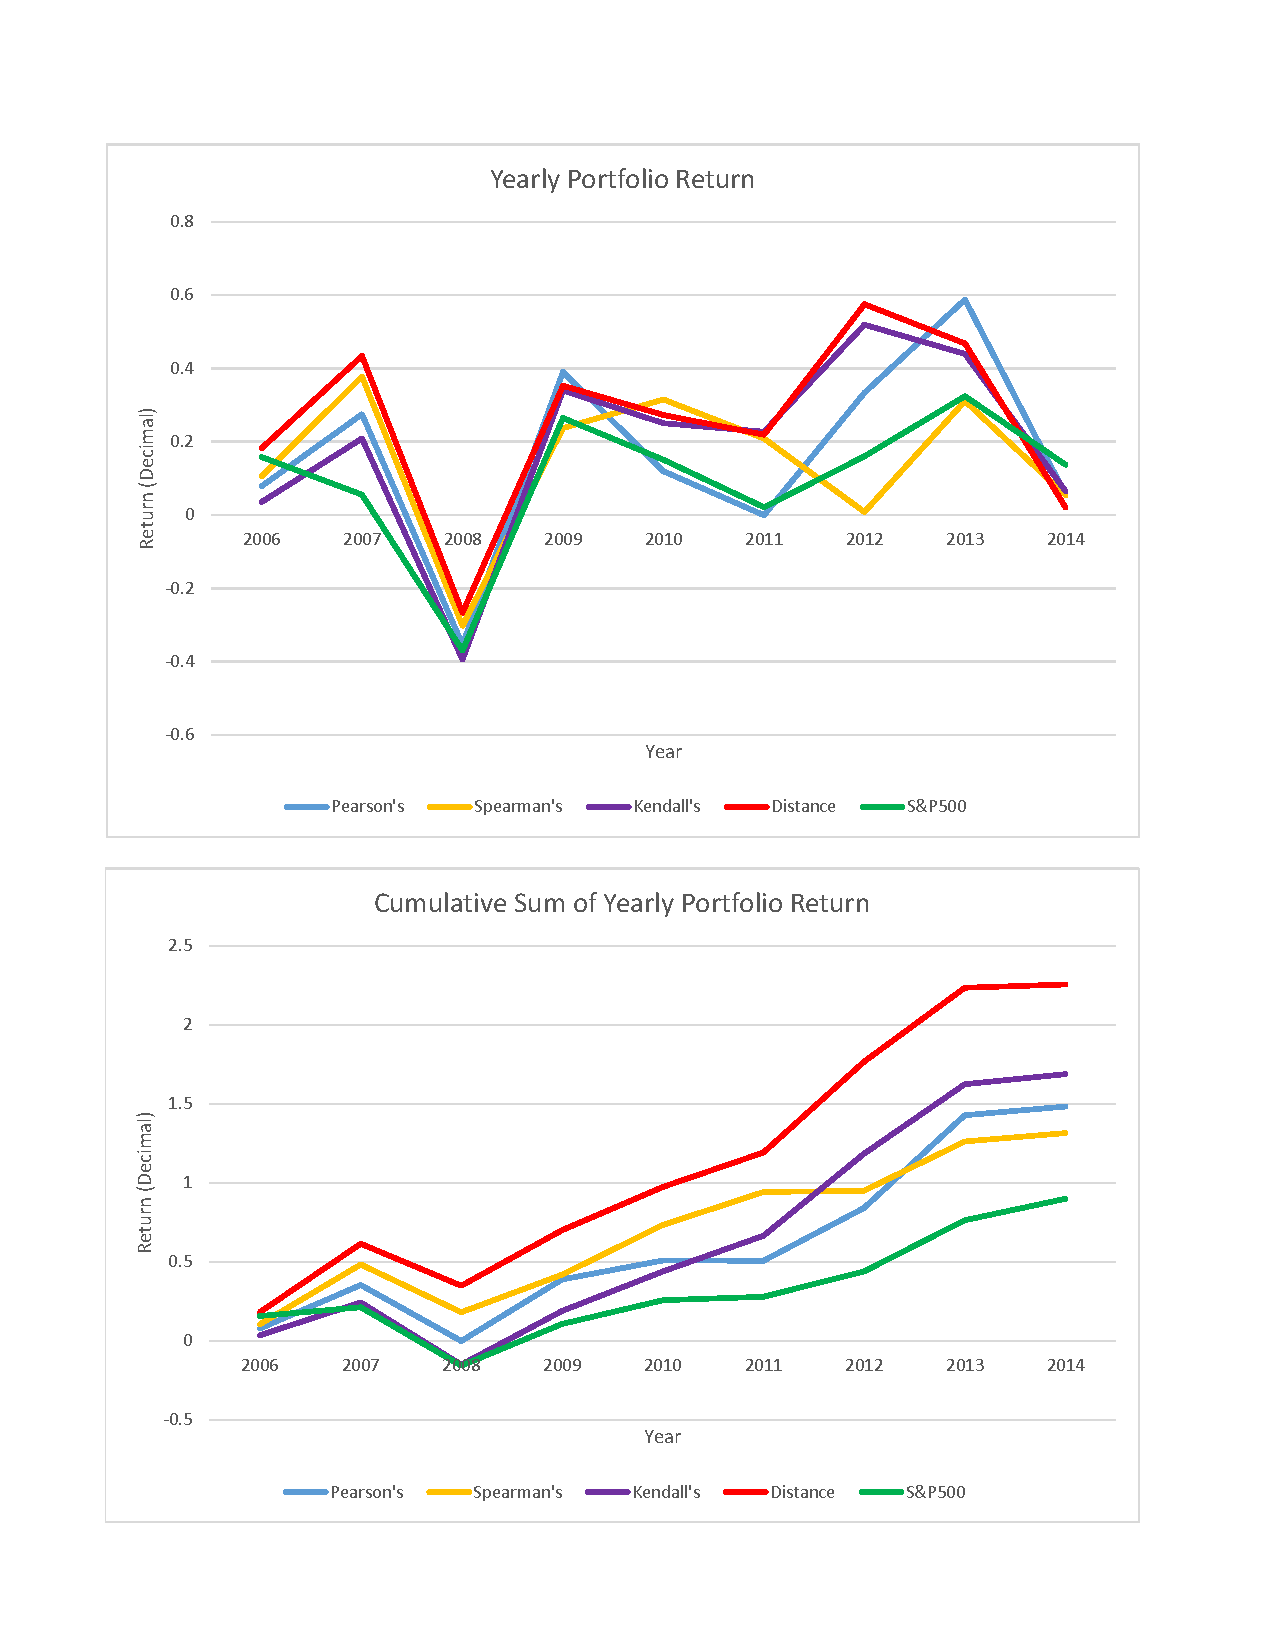
\includegraphics[width=1\linewidth]
		{ch-usage/figures/Results_YearlyReturns.pdf}
		\caption[Yearly and cumulative performance of the selected portfolios 
		and the S\&P 500.]{Yearly and cumulative performance of the selected 
		portfolios and the S\&P 500. Note that the ``yearly'' returns for 2006 
		and 2014 are low because the data begins on 3/14/2006 and ends on 
		5/13/2004; as such, those returns do not reflect a full year of data. 
		The associated data may be found in Table~\ref{tab:usage:returns}.}
		\label{fig:usage:returns}
	\end{center}
\end{figure}




\begin{landscape}
\tablespacing
\begin{longtable}{p{0.15\linewidth}p{0.15\linewidth}p{0.05\linewidth}
p{0.05\linewidth}p{0.05\linewidth}p{0.05\linewidth} 
p{0.05\linewidth}p{0.05\linewidth}p{0.05\linewidth} 
p{0.05\linewidth}p{0.05\linewidth}p{0.05\linewidth} 
p{0.05\linewidth}}
	
	% First page heading
	\caption[Yearly returns of the portfolios selected from the numerical 
	correlation graphs.]{Yearly returns (in decimal) of the portfolios selected 
	from the numerical correlation graphs.} 
	\label{tab:usage:returns}\\
	\toprule
	\textbf{Graph Type} & \textbf{Portfolio} & \textbf{2006} 
	& \textbf{2007} & \textbf{2008} & \textbf{2009} & 
	\textbf{2010} & \textbf{2011} & \textbf{2012} & 
	\textbf{2013} & \textbf{2014} \\
	\midrule
	\endfirsthead
	
	% Future page heading
	\caption[]{(continued)}\\
	\toprule
	\textbf{Graph Type} & \textbf{Portfolio} & \textbf{2006} 
	& \textbf{2007} & \textbf{2008} & \textbf{2009} & 
	\textbf{2010} & \textbf{2011} & \textbf{2012} & 
	\textbf{2013} & \textbf{2014} \\
	\midrule
	\endhead
	
	% Page footer
	\midrule
	\multicolumn{11}{r}{(Continued on next page)}\\
	\endfoot
	
	% Last page footer
	\bottomrule
	\endlastfoot

	S\&P 500 \newline (CONTROL) & \textbf{Total} & 
	0.158&0.055&-0.37&0.265&0.151&0.021&0.16&0.324&0.137\\
	
	\cmidrule[0.1pt](l{0.5em}r{0.5em}){1-11}	
	
	Pearson's &CI&0.041&0.226&-0.686&1.099&0.041&0.147&0.274&0.637&0.011\\
	&GILD&0.056&0.417&0.111&-0.154&-0.162&0.129&0.795&1.045&0.069\\
	&SYK&0.15&0.362&-0.46&0.267&0.079&-0.061&0.121&0.393&0.073\\
	&TMO&0.276&0.274&-0.409&0.4&0.161&-0.188&0.432&0.758&0.057\\
	&VAR&-0.131&0.096&-0.328&0.337&0.479&-0.031&0.046&0.106&0.064\\
	&\textbf{Total}&0.078&0.275&-0.354&0.39&0.119&-0.001&0.333&0.588&0.055\\
	
	\cmidrule[0.1pt](l{0.5em}r{0.5em}){1-11}	
	
	Spearman's &HUM&0.122&0.362&-0.505&0.177&0.247&0.615&-0.206&0.523&0.184\\
	&LH&0.291&0.028&-0.147&0.162&0.175&-0.022&0.008&0.055&0.092\\
	&PRGO&0.096&1.041&-0.072&0.243&0.597&0.542&0.073&0.479&-0.144\\
	&SYK&0.15&0.362&-0.46&0.267&0.079&-0.061&0.121&0.393&0.073\\
	&VAR&-0.131&0.096&-0.328&0.337&0.479&-0.031&0.046&0.106&0.064\\
	&\textbf{Total}&0.106&0.378&-0.302&0.237&0.315&0.208&0.008&0.311&0.054\\
	
	\cmidrule[0.1pt](l{0.5em}r{0.5em}){1-11}	
	
	Kendall's&MCK&-0.039&0.297&-0.404&0.63&0.138&0.118&0.256&0.676&0.117\\
	&REGN&0.231&0.203&-0.24&0.317&0.358&0.688&2.086&0.609&0.03\\
	&SYK&0.15&0.362&-0.46&0.267&0.079&-0.061&0.121&0.393&0.073\\
	&UNH&-0.035&0.084&-0.543&0.148&0.199&0.422&0.086&0.41&0.04\\
	&VAR&-0.131&0.096&-0.328&0.337&0.479&-0.031&0.046&0.106&0.064\\
	&\textbf{Total}&0.035&0.209&-0.395&0.34&0.25&0.227&0.519&0.439&0.065\\
	
	%\cmidrule[0.1pt](l{0.5em}r{0.5em}){1-11}			
	\newpage
	
	Distance&JNJ&0.137&0.036&-0.078&0.113&-0.006&0.099&0.108&0.346&0.111\\
	(Most similar to 
	&PRGO&0.096&1.041&-0.072&0.243&0.597&0.542&0.073&0.479&-0.144\\
	visual graph)&REGN&0.231&0.203&-0.24&0.317&0.358&0.688&2.086&0.609&0.03\\
	&TMO&0.276&0.274&-0.409&0.4&0.161&-0.188&0.432&0.758&0.057\\
	&WAT&0.169&0.615&-0.536&0.691&0.254&-0.047&0.177&0.148&0.048\\
	&\textbf{Total}&0.182&0.434&-0.267&0.353&0.273&0.219&0.575&0.468&0.021\\
	
\end{longtable}
\bodyspacing
\end{landscape}
\section{Implications}
\label{sec:usage:implication}

((Real-world context such as portfolio construction. Was my intuition correct? (For example, if Google and Facebook stocks were both in the dataset, I would expect a link between the two to be maintained)))





\chapter{Conclusion and extensions\label{ch:conclusion}}

\section{Conclusion}
\label{sec:conclusion}

The proliferation of high-dimensional datasets has led analysts to rely on 
unverifiable numerical estimators. It would be useful to be able to construct 
high-dimensional visual correlation graphs as a way to verify numerical 
tests of dependence. Correlation graphs are important in portfolio selection as 
it is desirable to select stocks that are as uncorrelated as 
possible. However, high-dimensional visualization is problematic because there 
are too many potential plots to sort through manually; to be 
specific, there are ${n\choose 2} = n(n-1)/2$  plots where $n$ is the number of 
variables e.g. stocks that we are interested in. As a general solution to these 
issues, the visualization system described in Chapter~\ref{ch:visualizer} 
actively learns user preferences regarding 
their notion of visual correlation, applies 
the fitted classifier to unlabeled data, provides visualization tools for the 
active learning output, and outputs the difference among the visual graph $G$ 
and some given numerical graph $G^{\text{num}}$.

In this thesis, we focused specifically on the active learning and graph 
comparison components of the VS. We reviewed the two main approaches to active 
learning (efficient search through hypothesis space and 
exploiting clustering tendencies in data) and provided algorithms for 
different active learning methods in Chapter~\ref{ch:al}. These methods include 
uncertainty sampling, query by committee (for which we proposed a revised 
framework), query by bagging, and min-max clustering. A simulation study 
with parameters that mimicked the intended qualities of the VS indicated that 
uncertainty sampling would be the ideal active learning method to be 
implemented in stage 1 of the VC for usage in our financial application. 
Similarly, we discussed 
various graph summarization difference metrics, proposed a method to compare 
the distance metrics of various graph pairs in order to select the most 
similar pair, and demonstrated the viability of the proposed procedure in 
Chapter~\ref{ch:gc}. The graph summarization difference and similarity 
selection are outputs of the VS that may be applied to any graphs (not just 
correlation graphs) and, subsequently, may be applied to many different 
situations outside of finance.

Our financial data contains the daily prices of 43 different healthcare 
stocks that were treated to get rid of time-dependency. The data is split in 
half with the first half (1998 to 2006) used as ``training'' input and the 
second half (2006 to 2014) used as ``testing'' output. Various correlation 
coefficients were applied to the training set to create 
$\hat{G}^{i,\text{num}}$ for 
all $i \in \{1,...,4\}$ which correspond to the numerical correlation graphs 
for Pearson's, Spearman's, Kendall's, and distance correlation coefficient. We 
then ran the VS on the training set to determine the visual graph $\hat{G}$. 
After computing the difference between each graph pair 
$(\hat{G}^{i,\text{num}},\hat{G})$, the similarity selection procedure 
presented in Section~\ref{sec:gc:simulations} was used to find $\hat{G}^*$, the 
numerical graph $\hat{G}^{i,\text{num}}$ that most closely matches the visual 
graph $\hat{G}$. The algorithm selected $\hat{G}^{4,\text{num}}$, the distance 
correlation graph, as $\hat{G}^*$. 
Then the stock selection methodology described in 
Section~\ref{sec:usage:stockselection} was used to select a portfolio $P^i, i 
\in \{1,...,4\}$ of $k = 5$ stocks for each corresponding correlation graph 
$\hat{G}^{i,\text{num}}$. 
The testing set was used to compute yearly returns for each portfolio in a 
simulation of the ``buy and hold'' strategy. $P^* = P^4$, the 
distance correlation portfolio, is the consistent top performer. The 
application and results demonstrate the reliability and usefulness of the VS in 
a concrete application. Furthermore, the entire process is  
transparent, and results are reproducible given the recorded user responses 
to the stage 1 VS queries. Transparency and reproducibility are 
other important features of the VS that contribute towards the notion of 
``clean analysis''.

The visualization system presented in this thesis is an important step towards
streamlining the future of ``clean analysis''. It provides a systematic way for 
confirming and/or suggesting dependencies among variables that match the user's 
concept of visual dependence and allows others to easily understand and 
replicate the data analysis process. The VS both 
alleviates the problems associated with high-dimensional data analysis and 
allows the user to quickly identify where the numerical model may have fallen 
short of the ``true'' relationship between variables. Nevertheless, there are 
several places to develop further work in order to refine the system and 
improve our concept of ``clean analysis.'' % Conclusion
\section{Further extensions}

\subsection{Estimator selection}

((Estimator selection involves actively fitting the best model as opposed to ``checking'' a numerical model that’s been given. This problem is more difficult to define, and the value that the visualization system adds is not as concrete ))

\subsection{Outlier removal}

((Outliers are unavoidable in raw data and can skew results quite a bit. When can the system remove outliers? What criteria should it use? ))

\subsection{Edge-weighted graphs}

(( This is more of an extension on graphical models, but it is still related to estimator selection. In an edge-weighted graph, edges can be weighted depending on the type of conditional dependence – negative or positive, assign 1 or -1. 0 (no edge) still implies conditional independence ))

\subsection{Regression and graphical models}

Graphical models alleviate some of the problems associated with correlation graphs, but they have their own set of problems, as well. Let G=(V,E) be an undirected graph with vertices $V_1,...,V_d$ \textasciitilde $P$ (a $d$-dimensional distribution) and edges $E_{i,j}\in\{0,1\}$. We set $E_{i,j}=1$ when there is an edge between $V_i$ and $V_j$, and 0 otherwise. Do not draw an edge between $V_i$ and $V_j$ iff $V_i \perp V_j$ given $V_k$ where $k\in\{1,...,d\}$ \textbackslash $\{i,j\}$. In other words, do not draw an edge if
$$P(V_i,V_j|V_k)=P(V_i|V_k)P(V_j|V_k)$$

This is known as a graphical model. The drawback is the difficulty in empirically computing conditional distributions and the problems associated with fitting distributions to real data. While there are simplifications that can be made for plotting (Section \ref{sec:visualizer:scatterplot:conditional}), the solution is not always so clear. However, the conditional independence of graphical models is more of a global property than correlation is because, for every pair of variables, it conditions on all the remaining variables. Returning to the universe of Google, Apple, and Silicone stocks, conditioning Google on Silicone and Apple on Silicone makes the relationship between the two clearly uncorrelated. Thus, although conditional independence tends to be more difficult to determine, it will tend to give a sparser network that is more interpretable for the analyst. The search through the rest of the data space is akin to the way regressions are fitted.

There are many ways to numerically perform model selection, and regression is the most common. In low-dimensional settings (where there are more samples than explanatory variables), the most common way is to fit a least-squares linear regression and perform a hypothesis test on each coefficient. The F-test is another useful tool for numerically informing the user if a regression model with more variables has significantly more explanatory power over a nested regression model. There are also ways to perform regression and model selection simultaneously. The most common estimator is the Lasso, the Least Absolute Shrinkage and Selection Operator (Tibshirani 1996). The drawback to all these methods is that their theoretical properties tend to either be asymptotic or reliant on assumptions. The former is unsatisfactory since datasets in practice are typically of a fixed size, far from the number of samples to achieve desirable properties analogous to when the number of samples goes to infinity. The latter is unsatisfactory because these assumptions are typically hard to verify or provide convincing justifications of.

Analysts may choose to use correlation over graphical models or vice versa as each has its own niche to fill. It has been shown that the rebalancing method, which leverages independent stocks and is more akin to graphical models, outperforms the ``buy and hold'' method, which leverages negatively correlated variables and naturally lends itself to the correlation approach~\cite{liuh2016}. Due to the nature of our financial application, we choose to utilize graphical models in our analysis of the data, but it is important to understand that both methodologies have the same need for a program that makes high dimensional visualization simple. This allows the analyst to make an informed decision on whether to confirm or reject the numerical result and improves decision-making in the financial industry.

((There are many ways to produce this scatter plot. One way is to marginally plot one explanatory variable against the response variable. We experiment with another way where, similar to regression, we control for the behavior of all the other explanatory variables while making this scatter plot. ))

\subsection{Ordering}

As people interact with graphs, they maintain a ``mental map'' of the graph. Federico and Miksch note that the importance of the mental map depends on various factors such as the user preferences and tasks that they must complete~\cite{federico2016}. By ``mental map,'' Federico and Miksch mean that when users label a new graph, they remember the previous plots that they labeled~\cite{federico2016}. Supposing that the graphs that a program wants to show the user are already decided. Given a gradation of graphs (showing graphs that are most alike one after the other), users are less able to distinguish between differences than if they are shown graphs from different ends of the spectrum at different times~\cite{federico2016}. While their work primarily concerns itself with ordering graphs for interpretability, their results can be applied to scatter plots. To put it concisely, the scatter plot display itself is not the only thing that matter. The ordering of the display matters, as well, and it is best to show the plots in an order that allows users to distinguish the differences among graphs that they have already seen. By improving their understanding of the plots, careful display ordering advances the accuracy of user responses. User responses can be thought of as observations of the user’s true preferences, and the ordering of plots as a way to future tune the precision of the decision tree (Section~\ref{sec:visualizer:al}). 

\subsection{Line-up tests}

One of the pitfalls of data visualization is ``apophenia,'' a phenomenon where the user sees patterns in random noise. Part of the reason for this is due to the vagueness of defining ``independence'' on a non-uniform domain and range (Section~\ref{sec:visualizer:scatterplot:goodplot}). Wickham et al. propose a line-up protocol that is similar to the Rorscach test where subjects are asked to interpret abstract blots of ink~\cite{wickham2010}. In the line-up test, users are asked to identify the real data from a set of n plots where n – 1 plots are synthetically generated (Figure\ref{fig:visualizer:lineup}). Analogously in the context of the classification problem, the learner generates 4 ``uninteresting'' plots (following the proposed decision tree) with 1 ``interesting'' plot and asks the user if he/she can identify the interesting plot. If the user is able to consistently identify the interesting plot, it is an indication that the current decision tree is a close fit of the user’s preferences.

\begin{figure}[htb]
	\begin{center}
		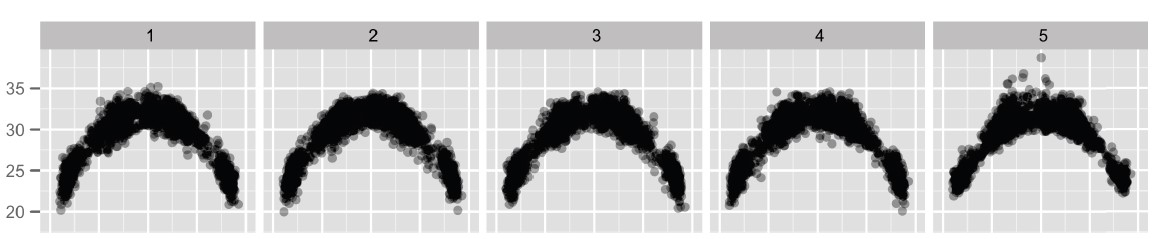
\includegraphics[width=1\linewidth]{ch-visualizer/figures/lineup}
		\caption[A line-up test for $n = 5$. ]{A line-up test for $n = 5$. Consistently identifying the raw data against the synthetic data indicates that the fitted model may not be good enough. Images from Wickham et al. 2010~\cite{wickham2010}}
		\label{fig:visualizer:lineup}
	\end{center}
\end{figure}


\subsection{Rejection classification}

So far, we have been discussing classification as black and white, interesting versus non-interesting. While interacting with the data visually, the user's concept of what's interesting in the specific dataset may evolve over time; at the beginning, they have no idea what the data looks like and where to set the bar for their own standards of dependence. There are several ways to take this into consideration. 

First, the visualization system could assign a weight to the analyst's responses by trial number where the last few plots are more valuable than the first few. However, this may destabilize cases where the user's preferences don’t end up changing, and it is difficult for the classifier to continuously rebalance each round given the weights (which, when applied to 2 black and white non-numerical responses, may also be vague). Secondly, the system can include an alternative option that allows the user to refuse to label a plot when it's too close to their decision boundary. This is welcome for the user who is not forced into making a decision he/she is uncertain about, but it is problematic for the learner as it causes the hypothesis space to remain unchanged rather than shrink. The point of the active learning segment is to have the user indicate to the learner which plots are interesting or not in order to let the computer better understand their preferences. By allowing for this option, the active learner may run for too long or return a poorly-defined tree. Finally, there is a way to consolidate the considerations within each methodology. The system can contain a third option that permits the user to ``recycle'' the plot. This allows to user to return to the plot later when he/she has learned more about what the data looks like and understand their own preferences better, and it ensures that the active learner will eventually receive data on the ambiguous plots that it has given the user to label. The main concern is that this could potentially de-balance an ordering procedure (Section~\ref{***EARLIER SECTION***}), but the system can strategically insert the recycled plot between two plots it differs from with the constraint that the insertion location is after the current plot. % Future work

\appendix % all chapters following will be labeled as appendices
\chapter{Implementation\label{ch:implementation}}

\lstset{basicstyle=\ttfamily\footnotesize,xleftmargin=0cm,breaklines=true,language=R}

\section{Code for Figure~\ref{fig:intro:meplot}, left}
\label{sec:appendicies:me1plot}
{\setstretch{1.0}
\begin{lstlisting}
# Generate a reproducible dataset and scale to [0,1]
set.seed(10)
x <- seq(0, 1, length.out = 100)
y <- rnorm(100)
y <- (y-min(y))/(max(y)-min(y))

# Sort the noise
y <- sort(y)
y <- y[c(seq(1,99,length.out=50), seq(100,2,length.out=50))]

# Local swapping
for(i in 4:96){
	y[(i-3):(i+3)] <- y[sample((i-3):(i+3))]
}

idx <- sample(1:100)
x <- x[idx]; y <- y[idx]

##################### Numerical feedback

## Fit linear regression
fitlm <- lm(y ~ x)
anova(fitlm)

## See if any coefficients are significant
summary(fitlm)

## See if residuals are normally-distributed
shapiro.test(fitlm$residuals)

## Correlation is not significantly different from zero
cor.test(x, y)

#################### Visual feedback
plot(x, y, pch = 16, cex = 2)
\end{lstlisting}
}


\section{Code for Figure~\ref{fig:intro:meplot}, right}
\label{sec:appendicies:me2plot}
{\setstretch{1.0}
\begin{lstlisting}
## Generate a reproducible dataset
set.seed(10)
n <- 50
x <- sort(rnorm(n))
sd.vec <- c(seq(1, 1.5, length.out = 50), seq(1.5, 1, length.out = 50))
y <- -x + 0.5*rnorm(n, sd = sd.vec)
y <- scale(y)

y[c(1,5,10)] <- min(y)
y[c(n-10, n-5, n)] <- max(y)

##################### Numerical feedback

## Fit linear regression
fitlm <- lm(y ~ x)
anova(fitlm)

## See if any coefficients are significant
summary(fitlm)

## See if residuals are normally-distributed
shapiro.test(fitlm$residuals) 

## Correlation is not significantly different from zero
cor.test(x, y)

#################### Visual feedback
plot(x,y, pch = 16, cex = 2)
\end{lstlisting}
}


\section{Code for Figure~\ref{fig:visualizer:cdf}}
\label{sec:appendicies:cdf}
{\setstretch{1.0}
\begin{lstlisting}
# Generate the dataset
set.seed(10)
n <- 500
x <- rnorm(n)
y <- rnorm(n)

# Plot data and apply CDF
par(mfrow=c(1,2))
plot(x,y, pch = 16, cex = 2)
plot(pnorm(x),pnorm(y),pch = 16, cex = 2)
\end{lstlisting}
}




\section{Uncertainty sampling}
\label{sec:appendicies:al:uncertainty}

Refer to Algorithm \ref{alg:al:methods:uncertainty}. 
{\setstretch{1.0}
\begin{lstlisting}

#' Uncertainty Sampling with bivariate labels
#'
#' @param X the full data matrix, n x d, including all unlabeled data
#' @param y a factor vector with 2 levels and NAs for unlabeled data
#' @param unlabel_index_c is a vector of n pre-selected (pooled) indices
#' @param classifier the classifier name
#' @param ... additional parameters for the active learning method
#'
#' @return an index to query
#' @export

uncertainty_sample <- function(X, y, unlabel_index_c, classifier,
	isR = FALSE, tout = NULL, ...){

	if (length(classifier) > 1 || missing(classifier) || is.null(classifier) || 
	is.na(classifier)) {
		stop("A single classifier is required for uncertainty sampling")
	}
	if (isR & is.null(tout)) {
		stop("Re-feed classifier_method return to next uncertainty_sample call")
	}	
	
	# Check that the classifier is compatible with uncertainty sampling
	c <- try(caret::modelLookup(classifier))
	if (!any(c$probModel)) {
		stop(classifier," must return posterior probabilities")
	}
	
	# Split X and y to retrieve labeled and unlabeled pairs
	unlabel_index <- which(is.na(y))
	x_lab <- X[-unlabel_index,]
	y_lab <- y[-unlabel_index]
	x_ulab <- X[unlabel_index_c,]
	
	if (!isR) {
		tout <- caret::train(x_lab,y_lab,classifier)
		p <- as.matrix(stats::predict(tout, newdata=x_ulab, type="prob"))
	} else {
		# Reuse the trained classifier from the classifier_method call
		# Of course, this only works since classifier = "rf", and the
		# classifier_method function also uses "rf"
		p <- as.matrix(stats::predict(tout, newdata=x_ulab, type="prob"))
	}
	
	# Return corresponding X index of posterior closest to 0.5
	p <- apply(p, 1, function(x) abs(x[1]-0.5))
	index <- unlabel_index_c[which(p == min(p))]
	if (length(index) > 1) index <- sample(index,1)
	index
}
\end{lstlisting}
}

\section{Query by committee}
\label{sec:appendicies:al:qbc}

Refer to Algorithm \ref{alg:al:methods:qbc2}. 
This implementation contains the functions for query selection and pruning. 
These functions are called by the main simulation engine (Appendix 
~\ref{sec:appendicies:al:simulations:simengine}) for the QBC method. 
The simulation engine is coded in such as way that it acts as the skeleton 
of the entire algorithm in Section~\ref{sec:al:methods:qbc}.

\subsection{Query selection}
{\setstretch{1.0}
\begin{lstlisting}

#' Query by Committee
#'
#' @param X the full data matrix, n x d, including all unlabeled data
#' @param y a factor vector with 2 levels and NAs for unlabeled data
#' @param unlabel_index_c is a vector of n pre-selected (pooled) indices
#' @param committee the list of committee classifiers
#' @param dis is the disagreement measure between committee classifications
#' @param isMajority is if overall classifier Majority Vote or Random Forest
#' @param tout is a list of trained classifiers from Majority Vote computation 
#' @param ... additional parameters for the active learning method
#'
#' @return a list with: an index to query AND committee predictions
#' @export

qbc_sample <- function(X, y, unlabel_index_c, committee,
	dis = "vote_entropy", isMajority = FALSE, tout= NULL, ...){
	
	if (missing(committee)||is.null(committee)) stop("A committee is required")
	if (isMajority & is.null(tout)) {
		stop("Re-feed the majority vote return to the next QBC_sample call")
	}
	
	unlabel_index <- which(is.na(y))
	x_lab <- X[-unlabel_index,]
	y_lab <- y[-unlabel_index]
	x_ulab <- X[unlabel_index_c,]
	p <- vector("list",length(committee))
	
	if (!isMajority) {
		for (i in 1:length(committee)) {
			tout <- caret::train(x_lab,y_lab,committee[i])
			p[[i]] <- predict(tout, newdata=x_ulab)
		}
	} else {
		# Reuse the trained classifiers from the majority vote call
		for (i in 1:length(committee)) {
			p[[i]] <- predict(tout[[i]], newdata=x_ulab)
		}
	}

	# Compute disagreement (functions from the activelearning package)
	d <- switch(dis,
		vote_entropy=vote_entropy(p),
		post_entropy=post_entropy(p),
		kullback=kullback(p)
		)
	
	index <- unlabel_index_c[which(d == max(d))]
	if (length(index) > 1) index <- sample(index,1)
	# Gather each committee's prediction
	pre <- rep(0,length(committee))
	for (i in 1:length(committee)) {
		# Predict function returns a factor
		pre[i] <- 
		as.numeric(as.character(p[[i]][which(unlabel_index_c==index)]))
	}
	
	list(index, pre)
}
\end{lstlisting}
}



\subsection{Committee pruning}
{\setstretch{1.0}
\begin{lstlisting}

#' Query by Committee (committee pruning function)
#'
#' @param X the full data matrix, n x d, including all unlabeled data
#' @param y a factor vector with 2 levels and NAs for unlabeled data
#' @param index is the classification of X[index,] which was queried
#' @param committee_pred is the list of committee predictions for index
#' @param k is the current iteration number that the AL_engine is on
#' @param pt is the pruning threshold (any error value above it is pruned)
#' @param err in (0 best,1 worst) is the committee's error-to-iteration ratio
#' @param is_prune is TRUE when pruning is desired, FALSE when not
#' @param ... additional parameters for the active learning method
#'
#' @return a list with: updated error AND indices to delete from the committee
#' @export

qbc_prune <- function(X,y,index,committee_pred,k,pt = 0.5,err,is_prune,...){

	if (missing(err) || is.null(err) || is.na(err)) {
		stop("Committee error ratio is required for QBC pruning")
	}
	prune <- vector() # Do not know how long prune will be until the end
	# Do not prune if committee size is 1 or if it's the first round
	if (length(committee_pred) == 1 | k == 1) {
		list(err, prune)
	} else {
		# Update error value
		for (i in 1:length(committee_pred)) {
			if (committee_pred[i] == y[index]) iv <- 0 else iv <- 1
			err[i] <- err[i] + (iv - err[i])/k
			if (err[i] > pt & is_prune) {
				prune <- c(prune,i)
			}
		}
		list(err, prune)
	}
}
\end{lstlisting}
}

\section{Vote entropy}
\label{sec:appendicies:al:entropy}

Refer to Section \ref{sec:al:methods:qbc}.
{\setstretch{1.0}
\begin{lstlisting}

#' Disagreement method (from activelearning package)
#' @importFrom itertools2 izip
#' @importFrom entropy entropy

vote_entropy <- function(x, type='class', entropy_method='ML'){

	it <- do.call(itertools2::izip, x)
	disagreement <- sapply(it, function(obs) {
		entropy::entropy(table(unlist(obs)), method=entropy_method)
	})
	disagreement
}
\end{lstlisting}
}



\section{Query by bagging}
\label{sec:appendicies:al:bagging}

Refer to Algorithm \ref{alg:al:methods:bagging}. 
{\setstretch{1.0}
\begin{lstlisting}

#' Query by Bagging
#'
#' @param X the full data matrix, n x d, including all unlabeled data
#' @param y a factor vector with 2 levels and NAs for unlabeled data
#' @param unlabel_index_c is a vector of n pre-selected (pooled) indices
#' @param classifier the name of a classification model
#' @param dis is the disagreement measure between committee classifications
#' @param num_class is the number of desired committee members
#' @param r in (0,1). r*(labeled set) = training set for each num_class round
#' @param ... additional parameters for the active learning method
#'
#' @return an index to query
#' @export

qbb_sample <- function(X, y, unlabel_index_c, classifier, 
	dis = "vote_entropy", num_class, r, ...){

	if(r<=0 || r>=1) stop("r must be in (0,1)")
	
	x_ulab <- X[unlabel_index_c,]
	
	# Randomly sample from the labeled set to create a classifier
	label_index <- which(!is.na(y))
	committee <- vector("list",num_class)
	for (i in 1:num_class) {
		idx <- sample(label_index,round(length(label_index)*r,0))
		committee[[i]] <- caret::train(X[idx,],y[idx],classifier)
	}
	
	# Utilize the resulting classifiers as a committee
	p <- vector("list",length(committee))
	for (i in 1:length(committee)) {
		p[[i]] <- stats::predict(committee[[i]], x_ulab)
	}
	
	# Compute disagreement (functions from the activelearning package)
	d <- switch(dis,
		vote_entropy=vote_entropy(p),
		post_entropy=post_entropy(p),
		kullback=kullback(p)
		)
	
	index <- unlabel_index_c[which(d == max(d))]
	if (length(index) > 1) index <- sample(index,1)
	index
}
\end{lstlisting}
}

\section{Min-max clustering}
\label{sec:appendicies:al:clustering}

Refer to Algorithm \ref{alg:al:methods:clustering}. 
{\setstretch{1.0}
\begin{lstlisting}

#' Min-Max Clustering
#'
#' @param X the full data matrix, n x d, including all unlabeled data
#' @param y a factor vector with 2 levels and NAs for unlabeled data
#' @param unlabel_index_c is a vector of n pre-selected (pooled) indices
#' @param dis is the distance measure between data
#' @param ... additional parameters for the active learning method
#'
#' @return an index to query
#' @export

cluster_sample <- function(X,y,unlabel_index_c,dis="euclidean",...){

	label_index <- which(!is.na(y))
	x_lab <- X[label_index,]
	y_lab <- y[label_index]
	x_ulab <- X[unlabel_index_c,]
	y_ulab <- y[unlabel_index_c]
	
	# Select the point furthest from the labeled set
	q <- rep(0,length(y_ulab))
	for (i in 1:length(y_ulab)) {
		min <- Inf
		for (j in 1:length(y_lab)) {
			temp <- cs_distance(X[unlabel_index_c[i],],X[label_index[j],],dis)
			if (min > temp) min <- temp
		}
		q[i] <- min
	}
	index <- unlabel_index_c[which(q==max(q))]
	if (length(index) > 1) index <- sample(index,1)
	index
}

# Main distance engine
cs_distance <- function(a,b,dis = "euclidean"){
	d <- switch(dis,
		euclidean=cs_euclidean_distance(a,b)
		)
}

# Euclidean Distance
cs_euclidean_distance <- function(a,b) {
	sqrt( sum( mapply( function(x,y) (x-y)^2, a, b)))
}
\end{lstlisting}
}

\section{AL simulation study}
\label{sec:appendicies:al:simulations}

Refer to Section \ref{sec:al:simulations}.
\subsection{MNIST data}
\label{sec:appendicies:al:simulations:data}
{\setstretch{1.0}
\begin{lstlisting}

# Load the MNIST dataset
load_mnist <- function() {
	load_image_file <- function(filename) {
		ret = list()
		f = file(filename,'rb')
		readBin(f,'integer',n=1,size=4,endian='big')
		ret$n = readBin(f,'integer',n=1,size=4,endian='big')
		nrow = readBin(f,'integer',n=1,size=4,endian='big')
		ncol = readBin(f,'integer',n=1,size=4,endian='big')
		x = readBin(f,'integer',n=ret$n*nrow*ncol,size=1,signed=F)
		ret$x = matrix(x, ncol=nrow*ncol, byrow=T)
		close(f)
		ret
	}
	load_label_file <- function(filename) {
		f = file(filename,'rb')
		readBin(f,'integer',n=1,size=4,endian='big')
		n = readBin(f,'integer',n=1,size=4,endian='big')
		y = readBin(f,'integer',n=n,size=1,signed=F)
		close(f)
		y
	}
	train <<- load_image_file('mnist/train-images-idx3-ubyte')	
	train$y <<- load_label_file('mnist/train-labels-idx1-ubyte')
}

# Plot a single digit
show_digitsmall <- function(arr196, col=gray(12:1/12), ...) {
	image(matrix(arr196, nrow=14)[,14:1], col=col, ...)
}

# Compress the MNIST dataset from 28x28 to 14x14
compressImg <- function(full){
	compressFour <- function(j){
		pixelvec = rep(NA,4)
		pixelvec[1] = full[2*j-1+floor((j-1)/14)*28];
		pixelvec[2] = full[2*j+floor((j-1)/14)*28];
		pixelvec[3] = full[2*j-1+28+floor((j-1)/14)*28];
		pixelvec[4] = full[2*j+28+floor((j-1)/14)*28];
		return(mean(pixelvec))
	}
	
	compress = unlist(lapply(1:196,compressFour))
	return(compress)
}

# Plot a multitude of digits
plotTable <- function(numRow,numCol,vec.labels,mat.images){
	vec.uniq = unique(vec.labels)
	par(mfrow=c(numRow,numCol),pty="s",mar = c(0.1,0.1,0.1,0.1))
	for(i in 1:length(vec.uniq)){
		tmpidx = which(vec.labels==vec.uniq[i])
		for(j in 1:length(which(vec.labels==vec.uniq[i]))){
			show_digitsmall(mat.images[tmpidx[j],],asp=TRUE)
		}
	}
}
\end{lstlisting}
}

\subsection{Simulation engine}
\label{sec:appendicies:al:simulations:simengine}

Although the function name is \texttt{AL\_engine}, this code corresponds to the 
simulation engine (all the \texttt{main} simulation file names are preceded by 
a \texttt{AL\_}). The actual active learning engine may be found in 
Appendix~\ref{sec:appendicies:al:simulations:alengine}.

{\setstretch{1,0}
\begin{lstlisting}

AL_engine <- function(X, y, y_unlabeled, al_method,
classifier_method, return_method, iter, n, ...){
	
	stopifnot(nrow(X) == length(y), is.matrix(X), is.factor(y), 
		length(levels(y)) == 2)
	idx <- which(is.na(y_unlabeled))
	stopifnot(length(idx) > 0, all(y[-idx] == y_unlabeled[-idx]), 
	  length(y)==length(y_unlabeled),is.factor(y_unlabeled))
	
	res <- rep(0,iter)
	
	### SET THE COMMITTEE HERE
	cm <- c("rf","nb","pls","svmRadialWeights")
	err<- rep(0,length(cm))
	
	for(i in 1:iter){
		# If QBC, the procedure is a little different....
		if (al_method == "qbc") {
			if (i != 1 & 
			as.character(substitute(classifier_method))=="qbc_majority") {
				# QBC Majority method re-trains committee after the oracle
				# Save computation time by passing those results to QBC algo
				next_sample <- active_learning(X=X,
					y=y_unlabeled,
					almethod=al_method,n=n, 
					committee = cm, 
					isMajority = TRUE, 
					tout = tout, ...)
			} else {
			next_sample <- active_learning(X=X, 
				y=y_unlabeled, almethod=al_method, 
				n=n, committee = cm, ...)
		}
		y_unlabeled[next_sample[[1]]] <- y[next_sample[[1]]]
		
		# Update error and prune committee
		if (i > iter/2) {
			prune <- active_learning(X=X, y=y_unlabeled, 
				almethod="qbc_prune", n = 0, 
				index=next_sample[[1]],
				committee_pred=next_sample[[2]], 
				k = i, err = err, is_prune = TRUE,
				...)
			err <- prune[[1]]
			# check if there's stuff to prune
			if (length(prune[[2]] != 0)) {
				cm <- cm[-unlist(prune[[2]])]
				err <- err[-unlist(prune[[2]])]
			}
		}
		else {
			prune <- active_learning(X=X, y=y_unlabeled, 
				almethod="qbc_prune", n = 0, 
				index=next_sample[[1]],
				committee_pred=next_sample[[2]], 
				k = i, err = err, is_prune = FALSE, 
				...)
			err <- prune[[1]]
		}
		
		# Compute residual error
		idx <- which(!is.na(y_unlabeled))
		tout <- classifier_method(X[idx,], y_unlabeled[idx], committee = cm)
		res[i] <- return_method(tout, X, y, committee = cm)
	}
	# Everything else (not QBC)
	else {
        if (i != 1 & al_method == "us") {
	        # classifier_method re-trains random forest after the oracle
	        # Save computation time by passing those results to US algo
	        # Of course, this only works since classifier = "rf", and the
	        # classifier_method function also uses "rf"
	        next_sample <- active_learning(X,
		        y_unlabeled, al_method, n, 
		        isR = TRUE, tout = tout, ...)
        } else {
	        next_sample <- active_learning(X, y_unlabeled, al_method, n, ...)
        }
 		y_unlabeled[next_sample] <- y[next_sample]
		
		# Compute residual error
		idx <- which(!is.na(y_unlabeled))
		tout <- classifier_method(X[idx,], y_unlabeled[idx])
		res[i] <- return_method(tout, X, y)
		}
	}
	res
}
\end{lstlisting}
}

The AL engine without committee pruning (\texttt{AL\_engine\_noprune}) is the 
exact same as \texttt{AL\_engine} with the committee pruning section removed. 
\texttt{AL\_engine\_noprune} is called by the two QBC methods which do not 
utilize committee pruning (see Table~\ref{tab:al:simulations} where 
\textit{C\_Pruning} = F). For the sake of completeness, the code is also 
included below.

{\setstretch{1.0}
\begin{lstlisting}

AL_engine_noprune <- function(X, y, y_unlabeled, al_method,
classifier_method, return_method, iter, n, ...){
	
	stopifnot(nrow(X) == length(y), is.matrix(X), is.factor(y), 
	length(levels(y)) == 2)
	idx <- which(is.na(y_unlabeled))
	stopifnot(length(idx) > 0, all(y[-idx] == y_unlabeled[-idx]), 
	length(y)==length(y_unlabeled),is.factor(y_unlabeled))
	
	res <- rep(0,iter)
	
	### SET THE COMMITTEE HERE
	cm <- c("rf","nb","pls","svmRadialWeights")
	err<- rep(0,length(cm))
	
	for(i in 1:iter){
		# If QBC, the procedure is a little different....
		if (al_method == "qbc") {
			if (i != 1 & 
			as.character(substitute(classifier_method))=="qbc_majority") {
				# QBC Majority method re-trains committee after the oracle
				# Save computation time by passing those results to QBC algo
				next_sample <- active_learning(X=X,
					y=y_unlabeled,
					almethod=al_method,n=n, 
					committee = cm, 
					isMajority = TRUE, 
					tout = tout, ...)
			} else {
			next_sample <- active_learning(X=X,
				y=y_unlabeled, almethod=al_method, 
				n=n, committee = cm, ...)
		}
		y_unlabeled[next_sample[[1]]] <- y[next_sample[[1]]]
		
		# Compute residual error
		idx <- which(!is.na(y_unlabeled))
		tout <- classifier_method(X[idx,], y_unlabeled[idx], committee = cm)
		res[i] <- return_method(tout, X, y, committee = cm)
	}
	# Everything else (not QBC, not US)
	else {
		if (i != 1 & al_method == "us") {
			# classifier_method re-trains random forest after the oracle
			# Save computation time by passing those results to US algo
			# Of course, this only works since classifier = "rf", and the
			# classifier_method function also uses "rf"
			next_sample <- active_learning(X, 
				y_unlabeled, al_method, n, 
				isR = TRUE, tout = tout, ...)
		} else {
		next_sample <- active_learning(X, y_unlabeled, al_method, n, ...)
		}
		y_unlabeled[next_sample] <- y[next_sample]
		
		# Compute residual error
		idx <- which(!is.na(y_unlabeled))
		tout <- classifier_method(X[idx,], y_unlabeled[idx])
		res[i] <- return_method(tout, X, y)
		}
	}
	res
}
\end{lstlisting}
}

\subsection{AL algorithm engine}
\label{sec:appendicies:al:simulations:alengine}
{\setstretch{1.0}
\begin{lstlisting}

#' Main active learning engine
#'
#' The missing labels in y are denoted by NA.
#' This method takes X as a matrix of all the data
#'
#' @param X the full data matrix, n x d, including all unlabeled data
#' @param y a factor vector with 2 levels and NAs for unlabeled data
#' @param almethod the AL method name
#' @param n is the number of unlabeled points to be "pooled"
#' @param ... additional parameters for the active learning method
#'
#' @return an index corresponding to the row of X to learn the label of next
#' @export

active_learning <- function(X, y, almethod = "us", n, ...){

	stopifnot(nrow(X) == length(y), is.matrix(X), any(is.na(y)),
	is.factor(y), length(levels(y)) == 2)
	
	if (n == 0) {
		unlabel_index_c <- which(is.na(y))
	} else unlabel_index_c <- sample(which(is.na(y)), n)
	
	switch(almethod,
		us=uncertainty_sample(X,y,unlabel_index_c, ...),
		rs=random_sample(unlabel_index_c, ns = 1, ...),
		qbc=qbc_sample(X,y,unlabel_index_c, ...),
		qbb=qbb_sample(X,y,unlabel_index_c,...),
		qbc_prune=qbc_prune(X=X, y=y, ...),
		cluster=cluster_sample(X,y,unlabel_index_c, ...)
		)
}
\end{lstlisting}
}

\subsection{Simulator (main)}
\label{sec:appendicies:al:simulations:results}

Finally, the main simulator is what calls the simulation engine 25 times 
(trials) for each active learning method with the parameters described in 
Table~\ref{tab:al:simulations} and collects the results.

{\setstretch{1.0}
\begin{lstlisting}

setwd("---simulation file path---")
# NOTE: AL_header.R loads the simulation R package
# External installation via devtools::install_github("amytian789/thesis-al")
# Local installation via devtools::load_all("---package path---")
source("main/AL_header.R")
source("main/AL_engine.R")
source("main/AL_engine_noprune.R")
source("main/AL_data.R")




################################## Overall classifier and return methods

# MAIN class.model that will train on the data once AL selection is completed
# X and y contain labeled points
classifier_method <- function(X, y, ...) {
	caret::train(X,y,method="rf")
}

# MAIN prediction method for the data once AL selection is completed
# X contains all points to predict
classifier_predict <- function(classifier, X, ...) {
	stats::predict(classifier, X)
}

# Majority Committee Vote classification model
# X and y contain labeled points
qbc_majority <- function(X, y, committee, ...) {
	tout <- vector("list",length(committee))
	for (i in 1:length(committee)){
		tout[[i]] <- caret::train(X,y,committee[i])
	}
	tout
}

# Generic error ratio
# X contain all points. y are known labels (unknown to the learning algorithm)
return_method <- function(classifier, X, y, ...) {
	p <- stats::predict(classifier, X)
	length(which(p != y))/length(y)
}

# QBC error ratio
# X contain all points. y are known labels (unknown to the learning algorithm)
qbc_m_return <- function(tout, X, y, committee, ...) {
	p <- vector("list",length(committee))
	for (i in 1:length(committee)) {
		p[[i]] <- predict(tout[[i]],newdata=X)
	}
	# Aggregate prediction
	ap <- rep(0,length(y))
	for (i in 1:length(y)){
		temp <- as.numeric(as.character(p[[1]][i]))
		for (j in 1:length(committee)){
			temp <- c(temp,as.numeric(as.character(p[[j]][i])))
		}
		# error checking if a value doesn't appear at all
		if (is.na(as.numeric(sort(table(temp),decreasing=TRUE)[2]))) {
			ap[i] <- as.numeric(names(sort(table(temp),decreasing=TRUE)[1]))
		} else {
			# pick one at random if there is a tie
			if (as.numeric(sort(table(temp),decreasing=TRUE)[1]) ==
			as.numeric(sort(table(temp),decreasing=TRUE)[2])){
				temp <- c(0,1)
				ap[i] <- sample(temp,1)
			} else {
				# Otherwise, insert the first one
				ap[i] <- as.numeric(names(sort(table(temp),decreasing=TRUE)[1]))
			}
		}
	}
	length(which(ap != y))/length(y)
}




################################ Set up the data

load_mnist()
names(train)

# Randomly select the dataset. a and b are the labels which we want to compare 
# (a,b in [0,10]. We are only interested bivariate classification)
a <- 7
b <- 9
n <- 250 # desired dataset size
init <- 10 # desired number of points to initialize with
set.seed(10)
idx <- c(sample(which(train$y == a),n/2),sample(which(train$y == b),n/2))
X <- train$x[idx,]
X <- t(apply(X,1,compressImg)) # compress from 28x28 to 14x14 pixels
y <- as.factor(train$y[idx]) # y contains the "true" labels. y is never seen by 
the AL algorithms 

# Randomly select the initial points given to the AL algorithms
y_unlabeled <- y
set.seed(10)
y_unlabeled[sample(1:n,n-init)] <- NA

# Visual representation of the data
plotTable(13,20,y,X)

rm(train)




###################################

s <- 15 # Number of random unlabeled points to "pool"
	# n = 0 indicates that the "pool" should sample from all data points
k <- 25 # Number of simulations to run
iter <- 50  # Number of AL algorithm iterations (the "budget")




# Classifier performance given all data is labeled
# pred <- classifier_method(X,y)
# perf_results <- rep(return_method(pred,X,y),iter)
# This has been shown to yield perfect results, so it is commented out

# Uncertainty Sampling
us_results <- matrix(0,nrow=k,ncol=iter)
for (i in 1:k){
	set.seed(i)
	us_results[i,] <- AL_engine(X=X, y=y, 
		y_unlabeled=y_unlabeled, al_method = "us", 
		classifier_method = classifier_method, 
		return_method = return_method, 
		iter = iter, n = s, classifier = "rf")
	print(c("Trial ",i,"complete"))
}

# Query by Committee with "Majority Committee Vote" model
qbc_majority_results <- matrix(0,nrow=k,ncol=iter)
for (i in 1:k){
	set.seed(i)
	### To change the committee, you must set it in the AL_engine
	qbc_majority_results[i,] <- AL_engine(X=X, y=y, 
		y_unlabeled=y_unlabeled, al_method = "qbc", 
		classifier_method = qbc_majority,
		return_method = qbc_m_return, 
		iter = iter, n = s, dis = "vote_entropy", pt = 0.5)
	print(c("Trial ",i,"complete"))
}

# Query by Committee with "Majority Committee Vote" model
# no pruning
qbc_majority_noprune_results <- matrix(0,nrow=k,ncol=iter)
for (i in 1:k){
	set.seed(i)
	### To change the committee, you must set it in the AL_engine_noprune
	qbc_majority_noprune_results[i,] <- AL_engine_noprune(X=X,
		y=y, y_unlabeled=y_unlabeled, al_method = "qbc", 
		classifier_method = qbc_majority, 
		return_method = qbc_m_return, 
		iter = iter, n = s, dis = "vote_entropy", pt = 0.5)
	print(c("Trial ",i,"complete"))
}

# Query by Committee with overall "Random Forest" model
qbc_rf_results <- matrix(0,nrow=k,ncol=iter)
for (i in 1:k){
	set.seed(i)
	### To change the committee, you must set it in the AL_engine
	qbc_rf_results[i,] <- AL_engine(X=X, y=y, 
		y_unlabeled=y_unlabeled, al_method = "qbc", 
		classifier_method = classifier_method, 
		return_method = return_method, 
		iter = iter, n = s, dis = "vote_entropy", pt = 0.5)
	print(c("Trial ",i,"complete"))
}

# Query by Committee with overall "Random Forest" model
# no pruning
qbc_rf_noprune_results <- matrix(0,nrow=k,ncol=iter)
for (i in 1:k){
	set.seed(i)
	### To change the committee, you must set it in the AL_engine_noprune
	qbc_rf_noprune_results[i,] <- AL_engine_noprune(X=X, y=y, 
		y_unlabeled=y_unlabeled, al_method = "qbc", 
		classifier_method = classifier_method, 
		return_method = return_method, 
		iter = iter, n = s, dis = "vote_entropy", pt = 0.5)
	print(c("Trial ",i,"complete"))
}

# Query by Bagging
qbb_results <- matrix(0,nrow=k,ncol=iter)
for (i in 1:k){
	set.seed(i)
	qbb_results[i,] <- AL_engine(X=X, y=y, 
		y_unlabeled=y_unlabeled, al_method = "qbb", 
		classifier_method = classifier_method,
		return_method = return_method, 
		iter = iter,n = s,classifier="rf", 
		dis = "vote_entropy", num_class=5, r=0.75)
	print(c("Trial ",i,"complete"))
}

# Min-Max Clustering
cluster_results <- matrix(0,nrow=k,ncol=iter)
for (i in 1:k){
	set.seed(i)
	cluster_results[i,] <- AL_engine(X=X, y=y,
		y_unlabeled=y_unlabeled, al_method = "cluster", 
		classifier_method = classifier_method, 
		return_method = return_method, 
		iter = iter,n = s, dis = "euclidean")
	print(c("Trial ",i,"complete"))
}

# Random Sampling
random_results <- matrix(0,nrow=k,ncol=iter)
for (i in 1:k){
	set.seed(i)
	random_results[i,] <- AL_engine(X, y, y_unlabeled, 
		al_method = "rs", classifier_method, return_method, 
		iter, s)
	print(c("Trial ",i,"complete"))
}

# Average
us_vec <- apply(us_results,2,mean)
random_vec <- apply(random_results,2,mean)
qbc_majority_vec <- apply(qbc_majority_results,2,mean)
qbc_majority_noprune_vec <- apply(qbc_majority_noprune_results,2,mean)
qbc_rf_vec <- apply(qbc_rf_results,2,mean)
qbc_rf_noprune_vec <- apply(qbc_rf_noprune_results,2,mean)
qbb_vec <- apply(qbb_results,2,mean)
cluster_vec <- apply(cluster_results,2,mean)

# Select best QBC output (with pruning)
if (length(which(qbc_majority_vec < qbc_rf_vec)) > 
length(which(qbc_majority_vec > qbc_rf_vec))){
	qbc_prune_vec <- qbc_majority_vec
} else if (length(which(qbc_majority_vec < qbc_rf_vec)) < 
length(which(qbc_majority_vec > qbc_rf_vec))){
	qbc_prune_vec <- qbc_rf_vec
} else{
	# select one at random
	set.seed(1)
	rr <- sample(c(0,1),1)
	if (rr == 0) qbc_prune_vec <- qbc_majority_vec
	else qbc_prune_vec <- qbc_rf_vec
}
# Select best QBC output (with no pruning)
if (length(which(qbc_majority_noprune_vec < qbc_rf_noprune_vec)) > 
length(which(qbc_majority_noprune_vec > qbc_rf_noprune_vec))){
	qbc_noprune_vec <- qbc_majority_noprune_vec
} else if (length(which(qbc_majority_noprune_vec < qbc_rf_noprune_vec)) < 
length(which(qbc_majority_noprune_vec > qbc_rf_noprune_vec))){
	qbc_noprune_vec <- qbc_rf_noprune_vec
} else{
	# select one at random
	set.seed(2)
	rr <- sample(c(0,1),1)
	if (rr == 0) qbc_noprune_vec <- qbc_majority_noprune_vec
	else qbc_noprune_vec <- qbc_rf_noprune_vec
}
# Select best overall QBC output
if (length(which(qbc_prune_vec < qbc_noprune_vec)) > 
length(which(qbc_prune_vec > qbc_noprune_vec))){
	qbc_vec <- qbc_prune_vec
} else if (length(which(qbc_prune_vec < qbc_noprune_vec)) < 
length(which(qbc_prune_vec > qbc_noprune_vec))){
	qbc_vec <- qbc_noprune_vec
} else{
	# select one at random
	set.seed(3)
	rr <- sample(c(0,1),1)
	if (rr == 0) qbc_vec <- qbc_prune_vec
	else qbc_vec <- qbc_noprune_vec
}


################################### Plot the results

date <- Sys.Date()
pdf(file=paste0("results/results_", date, ".PDF"), 
height = 6, width = 10)

### Plot all AL performance
ymax <- max(c(us_vec, random_vec, qbc_vec,cluster_vec))
graphics::plot(1:iter, qbc_vec, ylim=c(0,ymax), lwd=2, type="l", 
	main="AL Error Ratios with Random Forest classification model*", 
	xlab="Iterations", ylab="Error", col = "green")
mtext("*Query by Committee uses Majority Committee Vote classification model")
graphics::lines(1:iter, random_vec, lwd = 2, col = "red")
graphics::lines(1:iter, us_vec, lwd = 2, col = "black")
graphics::lines(1:iter, qbb_vec, lwd = 2, col = "blue")
graphics::lines(1:iter, cluster_vec, lwd = 2, col = "orange")
graphics::legend(x="bottomleft",lwd=2,cex = 0.75,
	title="Active Learning method",
	legend = c("Random Sampling","Uncertainty Sampling",
	"Query by Committee (best)","Query by Bagging","Min-Max Clustering"),
	col=c("red","black","green","blue","orange"))

### Plot QBC performance
graphics::plot(1:iter,qbc_majority_vec,ylim=c(0,ymax),lwd=2,type="l"
	,main="Query by Committee AL Error Ratio with various parameters", 
	xlab="Iterations", ylab="Error", col = "red")
graphics::lines(1:iter, qbc_majority_noprune_vec, lwd = 2, lty = 2, col = "red")
graphics::lines(1:iter, qbc_rf_vec, lwd = 2, col = "blue")
graphics::lines(1:iter,qbc_rf_noprune_vec, lwd = 2, lty = 2, col = "blue")
graphics::legend(x="bottomleft",lwd=2,cex = 0.75,
	title="Main Classifier | Committee Pruning?",
	legend=c("Majority Committee Vote | Yes", "Majority Committee Vote | No",
	"Random Forest | Yes", "Random Forest | No"),
	col=c("red","red","blue","blue"), lty=c(1,2,1,2))

graphics.off()
save.image(file = paste0("results/results_", date, ".RData"))
\end{lstlisting}
}
















\section{Graph summarization engine}
\label{sec:appendicies:gc:engine}

Given graphs $\hat{G^1}=(V^1,E^1)$ and $\hat{G^2}=(V^2,E^2)$, the graph 
summarization engine computes the vector $d^{1,2}$ which 
contains the difference between $\hat{G^1}$ and $\hat{G^2}$ with the various 
summarization metrics described in Section~\ref{sec:gc:methods}. After the 
graph summarization engine code, the distance engine function is also included. 
The distance engine is called by the graph comparison engine in order to 
compute the distance between the two results (one from each graph) for a 
summarization method. Distance methods available are Euclidean distance, L1, 
L2, and Jaccard distance (for use with community only).

{\setstretch{1.0}
\begin{lstlisting}

# g1 and g2 are igraphs
# gSumm is a vector of strings corresponding to graph summarization methods
	### cen_deg = Centrality (degree)
	### cen_clo = Centrality (closeness)
	### cen_bet = Centrality (betweenness)
	### ast = Assortativity
	### com_rw = Community (random walk)
	### com_im = Community (infomap)
	### com_bet = Community (betweenness)
	### dis = distance matrix
	### eco = Edge connectivity
	### edh = Edge density histogram
# distf is the desired difference function

GC_engine <- function(g1, g2, gSumm, distf = "euclidean", ...){

	stopifnot(igraph::is_igraph(g1), igraph::is_igraph(g2), 
		igraph::gorder(g1) == igraph::gorder(g2),
		!is.null(gSumm))
	
	diff <- rep(0,length(gSumm))
	names(diff) <- rep("",length(gSumm))
	i <- 1
	
	# Centrality (degree)
	if ("cen_deg" %in% gSumm){
		a <- igraph::centr_degree(g1)$centralization
		b <- igraph::centr_degree(g2)$centralization
		
		diff[i] <- dist_engine(a,b,distf)
		names(diff)[i] <- "cen_deg"
		i <- i + 1
	}
	
	# Centrality (closeness)
	if ("cen_clo" %in% gSumm){
		a <- igraph::centr_clo(g1)$centralization
		b <- igraph::centr_clo(g2)$centralization
		
		diff[i] <- dist_engine(a,b,distf)
		names(diff)[i] <- "cen_clo"
		i <- i + 1
	}
	
	# Centrality (betweenness)
	if ("cen_bet" %in% gSumm){
		a <- igraph::centr_betw(g1)$centralization
		b <- igraph::centr_betw(g2)$centralization
		
		diff[i] <- dist_engine(a,b,distf)
		names(diff)[i] <- "cen_bet"
		i <- i + 1
	}
	
	# Assortativity
	if ("ast" %in% gSumm){
		a <- igraph::assortativity_degree(g1)
		b <- igraph::assortativity_degree(g2)
		
		if (is.nan(a)) a <- 0
		if (is.nan(b)) b <- 0
		
		diff[i] <- dist_engine(a,b,distf)
		names(diff)[i] <- "ast"
		i <- i + 1
	}
	
	# Community (random walk)
	if ("com_rw" %in% gSumm){
		a <- igraph::membership(igraph::cluster_walktrap(
			g1,steps=igraph::gorder(g1)/2))
		b <- igraph::membership(igraph::cluster_walktrap(
			g2,steps=igraph::gorder(g2)/2))
		
		diff[i] <- dist_engine(a,b,dist="jaccard")
		names(diff)[i] <- "com_rw"
		i <- i + 1
	}
	
	# Community (infomap)
	if ("com_im" %in% gSumm){
		a <- igraph::membership(igraph::cluster_infomap(g1))
		b <- igraph::membership(igraph::cluster_infomap(g2))
		
		diff[i] <- dist_engine(a,b,dist="jaccard")
		names(diff)[i] <- "com_im"
		i <- i + 1
	}
	
	# Community (betweenness)
	if ("com_bet" %in% gSumm){
		a <- igraph::membership(igraph::cluster_edge_betweenness(g1))
		b <- igraph::membership(igraph::cluster_edge_betweenness(g2))
		
		diff[i] <- dist_engine(a,b,dist="jaccard")
		names(diff)[i] <- "com_bet"
		i <- i + 1
	}
	
	# Distance matrix 
	if ("dis" %in% gSumm){
	    a <- distances(g1)
	    b <- distances(g2)
	    
	    # change from matrix -> vector for distance computation (by column)
	    # keep only 1 side of the matrix (both sides are the same)
	    # don't keep the values in the middle (since it's the same node)
	    a[a == Inf] <- 0
	    a <- a[upper.tri(a)]
	    b[b == Inf] <- 0
	    b <- b[upper.tri(b)]
	    
	    diff[i] <- dist_engine(a,b,distf) / (dist_engine(
		    rep(0,igraph::gorder(g1)-1),
		    seq(1,igraph::gorder(g1)-1,by=1),distf)
	    names(diff)[i] <- "dis"
	    i <- i + 1
	}
	
	# Edge connectivity 
	if ("eco" %in% gSumm){
		if (min(igraph::degree(g1)) != 0){
		a <- igraph::edge_connectivity(g1) / min(igraph::degree(g1))
		} else a <- 0
		if (min(igraph::degree(g2)) != 0){
		b <- igraph::edge_connectivity(g2) / min(igraph::degree(g2))
		} else b <- 0
		
		diff[i] <- dist_engine(a,b,distf)
		names(diff)[i] <- "eco"
		i <- i + 1
	}
	
	# Edge density histogram
	if ("edh" %in% gSumm){
		# histograms should be on the same scale. 
		# Use Freedman-Diaconis rule to determine bin width
		dd <- max(igraph::degree(g1),igraph::degree(g2))
		bw <- 2 * stats::IQR(igraph::degree(g1)) / igraph::gorder(g1)^(1/3)
		a <- graphics::hist(igraph::degree(g1),plot=FALSE,
			breaks=seq(0,dd+bw,by=bw))$counts / igraph::gorder(g1)
		b <- graphics::hist(igraph::degree(g2),plot=FALSE,
			breaks=seq(0,dd+bw,by=bw))$counts / igraph::gorder(g2)
		
		diff[i] <- dist_engine(a,b,distf)
		names(diff)[i] <- "edh"
		i <- i + 1
	}
	
	diff
}

######## Engine to call various distance computation methods
dist_engine <- function(a,b,dist = "euclidean", ...){
	switch(dist,
	euclidean=dist_euc(a,b),
	l1=dist_l1(a,b),
	l2=dist_l2(a,b),
	jaccard=dist_jac(a,b)
	)
}

# Euclidean distance
dist_euc <- function(a,b){
	sqrt( sum( mapply( function(x,y) (x-y)^2, a, b)))
}

# L1: Sum of absolute differences
dist_l1 <- function(a,b){
	sum ( mapply ( function(x,y) abs(x-y), a, b))
}

# L2: Sum of squared differences
dist_l2 <- function(a,b){
	sum ( mapply ( function(x,y) (x-y)^2, a, b))
}

# Jaccard distance
dist_jac <- function(a,b){
	1-clusteval::cluster_similarity(a,b,similarity="jaccard")
}
\end{lstlisting}

}


\section{Similarity selection}
\label{sec:appendicies:gc:similarity}

Given a base graph $\hat{G}$ and a set of graphs, the similarity selection 
method selects the graph $\hat{G}^*$ that is most similar to $\hat{G}$. The 
method is 
described in Section~\ref{sec:gc:simulations}.

{\setstretch{1.0}
\begin{lstlisting}

# Search for the "most similar" graph pair
# (characterized by having the lowest differences across the board)
#
# gc is a list of the differences among various graph pairs
# base is the index with which to start the search

GC_selection <- function(gc, base = 1){
	
	stopifnot(!is.null(gc))
	
	idx <- base
	old_idx <- 0
	while (old_idx != idx){
		old_idx <- idx
		idx <- best_c(gc,idx)
		#print(paste(old_idx,idx))
	}
	idx
}

# Select the next idx candidate given current best candidate
best_c <- function(gc, cand){

	for (i in 1:length(gc)){
		if (i != cand){
			if (sum(gc[[cand]] < gc[[i]]) < sum(gc[[cand]] > gc[[i]])){
				return( i )
			} else if (sum(gc[[cand]] < gc[[i]]) > sum(gc[[cand]] > gc[[i]])){
				# do nothing since the current candidate is better
			} else{
				return( sample(c(cand,i),1) )
			}
		}
	}
	return( cand )  
}
\end{lstlisting}
}


\section{GC simulation study}
\label{sec:appendicies:gc:simulations}

The graph comparison simulation study, which is used to demonstrate the 
viability of the 
proposed similarity selection model, is described in 
Section~\ref{sec:gc:simulations:algorithm}.

{\setstretch{1.0}
\begin{lstlisting}

setwd("---simulation file path---")
source("GC_engine.R")
source("dist_engine.R")
source("GC_selection.R")

library(igraph)
library(clusteval)

################################## Random sample given PDF

randomdraw <- function(n, prob){
	if(round(sum(prob),1) != 1 | length(which(prob<0)) > 0) 
	stop("Probability must be between 0 and 1")
	
	runningsum <- 0
	s <- runif(n)
		for (i in 1:n){
			for (j in 1:length(prob)){
				runningsum <- runningsum + prob[j]
				if (s[i] < runningsum){
				s[i] <- j
				break
			} 
		}
	}
	s
}

################################## Run simulations

# Create base graph
set.seed(10)
ss <- 50 # desired sample size (# of edges)
bg <- igraph::sample_gnm(20, ss)
bg_e <- igraph::as_edgelist(bg)

# Setting parameters
gSumm <- c("cen_deg","cen_clo","cen_bet","ast",
	"com_rw","com_im","com_bet","dis","eco","edh")
distf <- "l2"

msg <- rep(0,1000)
for (i in 1:1000) {
	set.seed(i)
	
	# g1: randomly swap 20% edges. 
	# Weight of each node is proportional to its degree
	g1 <- bg
	for (j in 1:(ss/5)) {
		idx <- sample(igraph::as_edgelist(g1),1)
		g1 <- igraph::delete_edges(g1,idx)
		prob <- igraph::degree(g1) / sum(igraph::degree(g1))
		nva <- sample(seq(1,length(prob),1),1)
		nvb <- randomdraw(1, prob)
		# make sure edges are not repeated
		while (g1[nva,nvb] == 1 | nva == nvb) nvb <- randomdraw(1,prob)
		g1 <- igraph::add_edges(g1, c(nva,nvb))
	}
	
	# g2: randomly swap 100% edges. 
	# Weight of each node is proportional to its degree
	g2 <- bg
	for (j in 1:(ss)) {
		idx <- sample(igraph::as_edgelist(g2),1)
		g2 <- igraph::delete_edges(g2,idx)
		prob <- igraph::degree(g2) / sum(igraph::degree(g2))
		nva <- sample(seq(1,length(prob),1),1)
		nvb <- randomdraw(1, prob)
		# make sure edges are not repeated
		while (g2[nva,nvb] == 1 | nva == nvb) nvb <- randomdraw(1,prob)
		g2 <- igraph::add_edges(g2, c(nva,nvb))
	}
	
	# Compute difference between (bg,g1), (bg,g2)
	gc <- vector("list",2)
	gc[[1]] <- GC_engine(g1=bg,g2=g1,gSumm=gSumm,distf=distf)
	gc[[2]] <- GC_engine(g1=bg,g2=g2,gSumm=gSumm,distf=distf)
	
	# Select the most similar graph pair
	msg[i] <- GC_selection(gc = gc, base = 1)
}
p1 <- length(which(msg == 1)) / length(msg)
p2 <- length(which(msg == 2)) / length(msg)
cat("Prob. of selecting (bg,g1):",p1,"\nProb. of selecting (bg,g2):", p2)

################################## Plot simulation graphs

bg$layout <- layout_in_circle # base graph
g1$layout <- layout_in_circle # from trial 1000 (seed = 1000)
g2$layout <- layout_in_circle # from trial 1000 (seed = 1000)

par(mfrow=c(1,3))
plot(bg)
plot(g1)
plot(g2)
\end{lstlisting}
}




















\section{Stock selection}
\label{sec:appendicies:usage:stockselection}

Given a correlation graph $G=(V,E)$, the program selects $k < |V|$ stocks 
(nodes) 
such that they are as uncorrelated with each other as possible. 
See Section~\ref{sec:usage:stockselection} and 
Algorithm~\ref{alg:usage:stockselection2}.

{\setstretch{1.0}
\begin{lstlisting}

# g_num is the numerical graph as an adjacency matrix
# k is the number of stocks to select
# dd is a vector of sample average price differences over time
# pd is the "drift" threshold ratio
# vv is a vector of sample average standard deviation
# pv is the "volatility" threshold ratio
#
# Returns a vector of selected stock tickers

stock_selection <- function(g_num, k, dd, pd = 0, vv, pv = 0){

	stopifnot(ncol(g_num) > k, pd >= 0, pv >= 0)
	
	# A) Drift
	rmv <- c()
	avgret <- sum(dd) / ncol(dd)
	for (i in 1:ncol(g_num)){
		if(dd[i] <= avgret * pd){
			rmv <- c(rmv, i)
		}
	}
	
	# B) Volatility
	avgvol <- sum(vv) / ncol(vv)
	for (i in 1:ncol(g_num)){
		if(vv[i] <= avgvol * pv){
			if(!(i %in% rmv)){
				rmv <- c(rmv, i)
			}
		}
	}
	g_num <- g_num[-rmv,-rmv]
	
	#print(g_num)
	
	# C) Main selection
	z <- combn(ncol(g_num),k)
	min <- Inf
	idx <- 0 
	for (i in 1:ncol(z)){
		c <- 0 # number of connections
		for (j in 1:(k-1)){
			for (l in (j+1):k){
				c <- c + g_num[z[j,i],z[l,i]]
			}
			if (c < min){
				min <- c
				idx <- i
			} else if (c == min){
				if (runif(1,0,1) > 0.5){
					min <- c
					idx <- i
				}
			} else{
				# do nothing
			}
		}
	}
	idx_s <- c()
	for (i in 1:length(z[,idx])){
		idx_s <- c(idx_s,colnames(g_num)[z[i,idx]])
	}
	idx_s
}
\end{lstlisting}
}










\section{Final application}
\label{sec:appendicies:usage:newanalysis}

Section~\ref{sec:usage:newanalysis} details the application procedure that is 
implemented below.

{\setstretch{1.0}
\begin{lstlisting}

setwd("---application file path---")
source("stock_selection.R")

library(Rsafd)
library(timeDate)
library(energy)
library(igraph)
library(clusteval)




################################## Read in data.

rd <- read.csv(file="HealthcareETF_prices.csv",sep=",",header=TRUE)
date <- as.timeDate(rd[,1])
data <- rd[,-1]

# avg drift and vol (computed in Excel)
dd <- read.csv(file="HealthcareETF_drift.csv",sep=",",header=TRUE)
vv <- read.csv(file="HealthcareETF_vol.csv",sep=",",header=TRUE)

# Remove seasonal and trend components of data
for (i in 1:ncol(data)){
	temp.ts <- Rsafd::timeSeries(data=data[,i],positions=date)
	# 261 is the avg number of workdays in a year
	temp.stl <- Rsafd::sstl(temp.ts, FREQ=261) 
	data[,i] <- temp.stl$rem@data
}

# Split data into testing and training sets
# Assume we are standing in the middle of the 1998 and 2014
data_train <- as.matrix(data[1:(nrow(data)/2),])
data_test <- as.matrix(data[(nrow(data)/2+1):nrow(data),])




################################## Create numerical graphs

# correlation threshold
t <- 0.15

# Pearson's correlation graph
m_pear <- matrix(0, ncol(data_train), ncol(data_train))
for (i in 1:(ncol(data_train)-1)){
	for (j in (i+1):ncol(data_train)){
		m_pear[i,j] <- stats::cor.test(data_train[,i],
			data_train[,j],method="pearson")$estimate
	}
}
g_pear <- igraph::make_empty_graph(n = ncol(data_train), directed = FALSE)
for (i in 1:(ncol(data_train)-1)){
	for (j in (i+1):ncol(data_train)){
		if (abs(m_pear[i,j]) > t){
			g_pear <- igraph::add_edges(g_pear, c(i,j))
		}
	}
}

# Spearman's correlation graph
m_spea <- matrix(0, ncol(data_train), ncol(data_train))
for (i in 1:(ncol(data_train)-1)){
	for (j in (i+1):ncol(data_train)){
		m_spea[i,j] <- stats::cor.test(data_train[,i],
			data_train[,j],method="spearman")$estimate
	}
}
g_spea <- igraph::make_empty_graph(n = ncol(data_train), directed = FALSE)
for (i in 1:(ncol(data_train)-1)){
	for (j in (i+1):ncol(data_train)){
		if (abs(m_spea[i,j]) > t){
			g_spea <- igraph::add_edges(g_spea, c(i,j))
		}
	}
}

# Kendall's correlation graph
m_ktau <- matrix(0, ncol(data_train), ncol(data_train))
for (i in 1:(ncol(data_train)-1)){
	for (j in (i+1):ncol(data_train)){
		m_ktau[i,j] <- stats::cor.test(data_train[,i],
			data_train[,j],method="kendall")$estimate
	}
}
g_ktau <- igraph::make_empty_graph(n = ncol(data_train), directed = FALSE)
for (i in 1:(ncol(data_train)-1)){
	for (j in (i+1):ncol(data_train)){
		if (abs(m_ktau[i,j]) > t){
			g_ktau <- igraph::add_edges(g_ktau, c(i,j))
		}
	}
}

# Distance correlation graph
m_dist <- matrix(0, ncol(data_train), ncol(data_train))
for (i in 1:(ncol(data_train)-1)){
	for (j in (i+1):ncol(data_train)){
		m_dist[i,j] <- energy::dcor.ttest(data_train[,i],
			data_train[,j])$estimate
	}
}
g_dist <- igraph::make_empty_graph(n = ncol(data_train), directed = FALSE)
for (i in 1:(ncol(data_train)-1)){
	for (j in (i+1):ncol(data_train)){
		if (abs(m_dist[i,j]) > t){
			g_dist <- igraph::add_edges(g_dist, c(i,j))
		}
	}
}

date <- Sys.Date()
save.image(file = paste0("corrgraphs_", date, ".RData"))




################################## Visualization system

devtools::install_github("linnylin92/graphicalModelEDA", 
	ref = "kevin",subdir = "graphicalModelEDA", force = T)
library(graphicalModelEDA)

# Run the VS
control_obj <- graphicalModelEDA::visualizer_control()
control_obj$parameter_list$initial_set <- 10 # faster initialization
res <- graphicalModelEDA::visualizer_system(data_train, trials = 15, 
	visualizer_control = control_obj, asp = T)

# Visual graph
g_visg <- graphicalModelEDA:::visual_graph(res, data_train)
plot(g_visg)

# Heat map
plot(res$results)

# Association navigator
plot(res$results, aes.list = aes.buja())

# Evaluate 100 random pairs and their associated plots
search_res <- graphicalModelEDA::automated_search(res,data_train)
# Histogram of predicted probabilities of correlation
plot(search_res) 
# Ordered predicted probabilities w/ the scatterplot pairs
cbind(search_res$pairs[order(search_res$values),], sort(search_res$values)) 
par(mfrow=c(2,3))
# Plot the top 5 most "interesting" pairs
graphicalModelEDA::selective_plot(search_res, dat, 
	selection = function(vec){ifelse(vec >= sort(vec, 
	decreasing = TRUE)[5], TRUE, FALSE)})

date <- Sys.Date()
save.image(file = paste0("visgraph_", date, ".RData"))




################################## Graph comparison

setwd("---GC file path---")
source("GC_engine.R")
source("dist_engine.R")
source("GC_selection.R")
setwd("---application file path---")

# Setting parameters
gSumm <- c("cen_deg","cen_clo","cen_bet","ast",
	"com_rw","com_im","com_bet","dis","eco","edh")
distf <- "l2"

# Compute difference between all graph pairs (g_visg is the "base")
gc <- vector("list",4)
gc[[1]] <- GC_engine(g1=g_visg,g2=g_pear,gSumm=gSumm,distf=distf)
gc[[2]] <- GC_engine(g1=g_visg,g2=g_spea,gSumm=gSumm,distf=distf)
gc[[3]] <- GC_engine(g1=g_visg,g2=g_ktau,gSumm=gSumm,distf=distf)
gc[[4]] <- GC_engine(g1=g_visg,g2=g_dist,gSumm=gSumm,distf=distf)

# Select the most similar graph pair
idx <- GC_selection(gc = gc, base = 3)

if (idx == 1){
	print("Pearson's")
} else if (idx == 2){
	print("Spearman's")
} else if (idx == 3){
	print("Kendall's")
} else{
	print("Distance")
}




################################## Stock selection

# Set parameters
k <- 5 # number of stocks to select
pd <- 2/3 # drift threshold ratio 
pv <- 2/3 # vol threshold ratio

# Pearson's
set.seed(10)
a_pear <- igraph::as_adjacency_matrix(g_pear)
colnames(a_pear) <- colnames(data)
s_pear <- stock_selection(a_pear, k, dd, pd, vv, pv)
s_pear

# Spearman's
set.seed(10)
a_spea <- igraph::as_adjacency_matrix(g_spea)
colnames(a_spea) <- colnames(data)
s_spea <- stock_selection(a_spea, k, dd, pd, vv, pv)
s_spea

# Kendall's
set.seed(10)
a_ktau <- igraph::as_adjacency_matrix(g_ktau)
colnames(a_ktau) <- colnames(data)
s_ktau <- stock_selection(a_ktau, k, dd, pd, vv, pv)
s_ktau

# Distance
set.seed(10)
a_dist <- igraph::as_adjacency_matrix(g_dist)
colnames(a_dist) <- colnames(data)
s_dist <- stock_selection(a_dist, k, dd, pd, vv, pv)
s_dist

# Visual
set.seed(10)
a_visg <- igraph::as_adjacency_matrix(g_visg)
colnames(a_visg) <- colnames(data)
s_visg <- stock_selection(a_visg, k, dd, pd, vv, pv)
s_visg

date <- Sys.Date()
save.image(file = paste0("portfolios_", date, ".RData"))




################################## Compare future performance 

# ON EXCEL: Use testing set to do this 
\end{lstlisting}
}
%\chapter{Printing and Binding\label{ch:printing}}

\section{Printing}

For the library copies of your dissertation, you must use archival quality printing and binding. This means acid-free paper, containing at least 25\% cotton fiber. Triangle Repocenter on Nassau Street in Princeton offers both 25\% cotton paper and 100\% cotton paper. Most people choose the 25\% cotton paper, and this is generally recommended by the binders. The 100\% copy paper is somewhat thicker and the extra expense is unnecessary. 

Triangle offers online submission of your printing and binding order at: \url{http://triangleprinceton.com/collegiatebinding/thesis/}. If you request binding from them, they will deliver the paper copies to Smith-Shattuck Bookbinding for you and allow you to pick up the completed copies at their store on Nassau Street. The whole process takes 2-3 business days, but check with them in advance during the busy thesis-printing season in April and May. 

Currently, your printed and bound dissertation copies can be single spaced. Only the electronic copy submitted to ProQuest must be double spaced. All copies must be printed single-sided, with specific margins. 

\section{Binding}

An archival-quality sewn binding is required for the library copies of your dissertation. Smith-Shattuck Bookbinding is highly recommended, and is used by most students. Triangle Repocenter will send your copies there for you, greatly simplifying the process, but you can call Smith-Shattuck with special requests. 

The ``library standard'' sewn binding is sufficient for the copies to be sent to Mudd Library. It uses a black buckram cloth cover, which is the most popular option. For extra copies for yourself and your family members, you can choose ``buckram roundback binding'', which adds decorative lines on the spine, and printing of the title and author on the front cover. For a small additional fee, you can include the Princeton University shield on the front cover and a ribbon bookmark. Leather covers are also available. See Smith-Shattuck's website for more details at: \url{http://www.thesisbookbinding.com/}. 


% Make the bibliography single spaced
\singlespacing
\bibliographystyle{plain}

% add the Bibliography to the Table of Contents
\cleardoublepage
\ifdefined\phantomsection
  \phantomsection  % makes hyperref recognize this section properly for pdf link
\else
\fi
\addcontentsline{toc}{chapter}{Bibliography}

% include your .bib file
\bibliography{thesis}

\end{document}

